% Options for packages loaded elsewhere
\PassOptionsToPackage{unicode}{hyperref}
\PassOptionsToPackage{hyphens}{url}
%
\documentclass[
  12pt,
]{article}
\usepackage{amsmath,amssymb}
\usepackage{iftex}
\ifPDFTeX
  \usepackage[T1]{fontenc}
  \usepackage[utf8]{inputenc}
  \usepackage{textcomp} % provide euro and other symbols
\else % if luatex or xetex
  \usepackage{unicode-math} % this also loads fontspec
  \defaultfontfeatures{Scale=MatchLowercase}
  \defaultfontfeatures[\rmfamily]{Ligatures=TeX,Scale=1}
\fi
\usepackage{lmodern}
\ifPDFTeX\else
  % xetex/luatex font selection
\fi
% Use upquote if available, for straight quotes in verbatim environments
\IfFileExists{upquote.sty}{\usepackage{upquote}}{}
\IfFileExists{microtype.sty}{% use microtype if available
  \usepackage[]{microtype}
  \UseMicrotypeSet[protrusion]{basicmath} % disable protrusion for tt fonts
}{}
\makeatletter
\@ifundefined{KOMAClassName}{% if non-KOMA class
  \IfFileExists{parskip.sty}{%
    \usepackage{parskip}
  }{% else
    \setlength{\parindent}{0pt}
    \setlength{\parskip}{6pt plus 2pt minus 1pt}}
}{% if KOMA class
  \KOMAoptions{parskip=half}}
\makeatother
\usepackage{xcolor}
\usepackage[margin=1in]{geometry}
\usepackage{graphicx}
\makeatletter
\def\maxwidth{\ifdim\Gin@nat@width>\linewidth\linewidth\else\Gin@nat@width\fi}
\def\maxheight{\ifdim\Gin@nat@height>\textheight\textheight\else\Gin@nat@height\fi}
\makeatother
% Scale images if necessary, so that they will not overflow the page
% margins by default, and it is still possible to overwrite the defaults
% using explicit options in \includegraphics[width, height, ...]{}
\setkeys{Gin}{width=\maxwidth,height=\maxheight,keepaspectratio}
% Set default figure placement to htbp
\makeatletter
\def\fps@figure{htbp}
\makeatother
\setlength{\emergencystretch}{3em} % prevent overfull lines
\providecommand{\tightlist}{%
  \setlength{\itemsep}{0pt}\setlength{\parskip}{0pt}}
\setcounter{secnumdepth}{5}
\usepackage{url}
\usepackage{setspace}
%\singlespacing
%\onehalfspacing
%\doublespacing
\usepackage{lineno}
%\linenumbers
\usepackage[belowskip=0pt,aboveskip=0pt]{caption}
\usepackage{relsize}
\newcommand{\Fmsy}{\ensuremath{F_{\text{MSY}}}\xspace}
\newcommand{\Fspr}[1]{\ensuremath{F_{\text{{#1}\%}}}\xspace}
\newcommand{\afrb}{Alaska Fishery Research Bulletin\xspace}
\newcommand{\ajms}{African Journal of Marine Science\xspace}
\newcommand{\amb}{Advances in Marine Biology\xspace}
\newcommand{\bms}{Bulletin of Marine Science\xspace}
\newcommand{\bjssf}{Bulletin of the Japanese Society of Scientific Fisheries\xspace}
\newcommand{\cb}{Conservation Biology\xspace}
\newcommand{\cjfas}{Canadian Journal of Fisheries and Aquatic Sciences\xspace}
\newcommand{\ea}{Ecological Applications\xspace}
\newcommand{\eer}{Evolutionary Ecology Research\xspace}
\newcommand{\elet}{Ecology Letters\xspace}
\newcommand{\emod}{Ecological Modelling\xspace}
\newcommand{\ebf}{Environmental Biology of Fishes\xspace}
\newcommand{\ff}{Fish and Fisheries\xspace}
\newcommand{\fo}{Fisheries Oceanography\xspace}
\newcommand{\fr}{Fisheries Research\xspace}
\newcommand{\fb}{Fishery Bulletin\xspace}
\newcommand{\ijms}{ICES Journal of Marine Science\xspace}
\newcommand{\iccat}{Collective Volume of Scientific Papers ICCAT\xspace}
\newcommand{\jae}{Journal of Animal Ecology\xspace}
\newcommand{\jai}{Journal of Applied Ichthyology\xspace}
\newcommand{\jdc}{Journal Du Conseil International Pour L'exploration De La Mer\xspace}
\newcommand{\jdcp}{Journal Du Conseil Permanent International Pour L'exploration De La Mer\xspace}
\newcommand{\jembe}{Journal of Experimental Marine Biology and Ecology\xspace}
\newcommand{\jfb}{Journal of Fish Biology\xspace}
\newcommand{\jsr}{Journal of Sea Research\xspace}
\newcommand{\jtb}{Journal of Theoretical Biology\xspace}
\newcommand{\jfrbc}{Journal of the Fisheries Research Board of Canada\xspace}
\newcommand{\jnwafs}{Journal of Northwest Atlantic Fisheries Science\xspace}
\newcommand{\mcf}{Marine and Coastal Fisheries: Dynamics, Management, and Ecosystem Science\xspace}
\newcommand{\mb}{Marine Biology\xspace}
\newcommand{\meps}{Marine Ecology Progress Series\xspace}
\newcommand{\mfr}{Marine Fisheries Review\xspace}
\newcommand{\mpb}{Marine Pollution Bulletin\xspace}
\newcommand{\najfm}{North American Journal of Fisheries Management\xspace}
\newcommand{\nzjmfr}{New Zealand Journal of Marine and Freshwater Research\xspace}
\newcommand{\pnas}{Proceedings of the National Academy of Sciences USA\xspace}
\newcommand{\rpvrciemm}{Rapports et Proc\`es-Verbaux des R\'eunions. Conseil Internationale pour l'Exploration de la Mer\xspace}
\newcommand{\rpvrcpiemm}{Rapports et Proc\`es-Verbaux des R\'eunions. Conseil Permanent Internationale pour l'Exploration de la Mer\xspace}
\newcommand{\rfbf}{Reviews in Fish Biology and Fisheries\xspace}
\newcommand{\sajms}{South African Journal of Marine Science\xspace}
\newcommand{\tafs}{Transactions of the American Fisheries Society\xspace}

\newcommand{\anzjs}{Australian \& New Zealand Journal of Statistics\xspace}
\newcommand{\as}{Applied Statistics\xspace}
\newcommand{\csda}{Computational Statistics \& Data Analysis\xspace}
\newcommand{\ees}{Environmental and Ecological Statistics\xspace}
\newcommand{\jas}{Journal of Applied Statistics\xspace}
\newcommand{\jabes}{Journal of Agricultural, Biological, and Environmental Statistics\xspace}
\newcommand{\jasa}{Journal of the American Statistical Association\xspace}
\newcommand{\jrssb}{Journal of the Royal Statistical Society. Series B\xspace}
\newcommand{\sm}{Statistics in Medicine}

\usepackage{float}
\usepackage{amsmath}
\usepackage{pdflscape}
\usepackage{hyperref}
\usepackage{xspace}
\usepackage{bm}
\usepackage{caption,graphics}
\usepackage{graphicx}
\usepackage{makecell}
\usepackage{lineno}
\linenumbers
\renewcommand\figurename{Figure.}
\captionsetup{labelsep=period, singlelinecheck=false}
\newcommand{\changesize}[1]{\fontsize{#1pt}{#1pt}\selectfont}
\renewcommand{\arraystretch}{1.5}
\renewcommand\theadfont{}
\usepackage{booktabs}
\usepackage{longtable}
\usepackage{array}
\usepackage{multirow}
\usepackage{wrapfig}
\usepackage{float}
\usepackage{colortbl}
\usepackage{pdflscape}
\usepackage{tabu}
\usepackage{threeparttable}
\usepackage{threeparttablex}
\usepackage[normalem]{ulem}
\usepackage{makecell}
\usepackage{xcolor}
\ifLuaTeX
  \usepackage{selnolig}  % disable illegal ligatures
\fi
\usepackage[]{natbib}
\bibliographystyle{cjfas2.bst}
\usepackage{bookmark}
\IfFileExists{xurl.sty}{\usepackage{xurl}}{} % add URL line breaks if available
\urlstyle{same}
\hypersetup{
  pdftitle={Evaluating the impact of log-normal bias-correction on a state-space stock assessment model},
  pdfauthor={Chengxue Li\^{}\{1,2,*\}; Jonathan J. Deroba\^{}1; Timothy J. Miller\^{}1; Christopher M. Legault\^{}1; Charles T. Perretti\^{}1},
  hidelinks,
  pdfcreator={LaTeX via pandoc}}

\title{Evaluating the impact of log-normal bias-correction on a
state-space stock assessment model}
\author{Chengxue Li\(^{1,2,*}\) \and Jonathan J.
Deroba\(^1\) \and Timothy J. Miller\(^1\) \and Christopher M.
Legault\(^1\) \and Charles T. Perretti\(^1\)}
\date{}

\begin{document}
\maketitle

\(^1\) Northeast Fisheries Science Center, Woods Hole Laboratory, 166
Water Street, Woods Hole, MA 02543 USA

\(^2\) Saltwater Inc., 733 N Street, Anchorage, AK 99501 USA

\(^*\)Corresponding author:
\href{mailto:chengxue.li@noaa.gov}{\nolinkurl{chengxue.li@noaa.gov}}

\pagebreak

\section*{Abstract}\label{abstract}
\addcontentsline{toc}{section}{Abstract}

In state-space stock assessment models, recruitment and numbers-at-age
are typically modeled as log-normal random variables, with bias
correction applied to ensure that their mean matches the expected mean
of the random variable. However, it remains unclear whether estimation
error in variance parameters, which influence bias correction,
propagates to estimates of population quantities. To address this, we
conducted simulation-estimation experiments to evaluate the effects of
bias correction for log-normal random variables and observations. We
found that applying bias correction on observations had minimal impact
on estimated population quantities, whereas applying bias correction on
the process had a significant effect. Specifically, when both
recruitment deviations and numbers-at-age transitions were treated as
random effects, substantial bias in estimated annual recruitments and
\(SSB\) was found when bias correction was excluded in the operating
model but applied in the estimation model. In contrast, not using bias
correction had limited negative effects. Thus, we recommend avoiding
bias correction for log-normal random variables in state-space models,
especially when multiple random-effects processes are modeled
simultaneously. (word count: 167)

\textbf{Keywords}: state-space models, random effects, bias correction,
recruitment, numbers-at-age transitions

\pagebreak

\section{Introduction}\label{introduction}

State-space population models include random and fixed effects, where
random effects represent random processes that are separable from
observation noise. Random effects now have been widely used to model a
variety of process errors in state-space stock assessments
\citep{Nielsen2014, Cadigan2015, Stock2021}. Perhaps the most common
random effects used in the state-space assessment model are deviations
on recruitment and numbers-at-ages 2+ (\(NAA\)). Recruitment and \(NAA\)
random effects are typically assumed to be log-normally distributed
\citep{Stock2021}.

Error modeled as normally distributed in log-space (i.e., log-normally
distributed), implies that error is multiplicative in natural space.
Log-normal error will increase the expected value of the population
process in natural space, where that increase is related to the variance
of the log-normal distribution. In order to ensure that this increase
does not occur, one can adjust the mean of the log-normal distribution,
known as ``bias-correction'' \citep{Methot2011}. Although there is not
universal agreement on whether bias-correction should be applied, an
important open question is the extent to which bias-correction affects
the accuracy of important assessment outputs such as recruitment and
spawning stock biomass (\(SSB\)). Here, we aim to address that question.

Bias, or estimation error, in derived population quantities can be
exacerbated by the nonlinear transformation (e.g., exponentiation) of a
random variable \citep{Thorson2016}. Whether applying a bias correction
term is sufficient to accurately recapture the true population
quantities remains an open question \citep{Deroba2016}. Methot and
Taylor (2011) claimed that population abundance is informed by
observations, which are never perfectly accurate and often exhibit
inter-annual variability in both quantity and quality. Ignoring this
source of variability can induce bias in the estimation of recruitment
variability, mean recruitment, and hence management quantities
\citep{Methot2011, Thorson2016}. An additional plug-in ``multiplier''
was proposed in maximum likelihood estimation to provide more accurate
recruitment estimates \citep{Methot2011, Thorson2016}. However, their
approach is not appropriate for state-space models. In their simulation
experiments, recruitment was treated as a penalized fixed effect and was
not integrated out of the likelihood for estimation. In addition, they
fixed the recruitment standard deviation (\(\sigma_{Rec}\)) to avoid
potential estimation error. In state-space models, however,
\(\sigma_{Rec}\) is estimated using the marginal maximum likelihood,
which can influence the utility of the log-normal adjustment and derived
population quantities.

In addition, evidence has indicated that when multiple processes are
treated as random effects in a state-space model, the process variation
may not be reliably partitioned for each process due to processes being
confounded with each other
\citep{Trijoulet2020, Li2024, Liljestrand2024}. Improperly estimated
process variance can induce inaccurate adjustment and subsequently bias
population quantities. Moreover, when bias correction is applied to
multiple random processes (e.g., recruitment and \(NAA\)), an
interaction among the parameters associated with these random processes
is introduced in the marginal maximum likelihood estimation. The impacts
of this interaction on derived quantities are not fully understood.

To understand the caveats of applying bias correction to log-normal
random variables, as well as observations, we designed a
simulation-estimation experiment based on three stocks {[}Georges Bank
(GB) yellowtail flounder: \emph{Limanda ferruginea}, Gulf of Maine (GoM)
haddock: \emph{Melanogrammus aeglefinus}, and Atlantic mackerel:
\emph{Scomber scombrus}{]}. We explored scenarios where either
recruitment only or both recruitment and \(NAA\) were treated as random
effects, with different autocorrelation structures. Overall, the goal of
this study is to provide guidance on bias-correction of log-normal
random effects and observations in state-space assessment models.

\section{Methods}\label{methods}

\subsection{Overview}\label{overview}

The Woods Hole Assessment Model (WHAM) is a state-space assessment model
(\url{https://timjmiller.github.io/wham}) \citep{Stock2021}. WHAM can
incorporate varying population and fishery processes, including
recruitment, \(NAA\), natural mortality, fishing selectivity, and survey
catchability \citep{Stock2021}. WHAM is currently used to manage various
stocks in the US northeast region. Below, we describe the population
processes and observations where a log-normal distribution is assumed.

\subsection{Population numbers-at-age}\label{population-numbers-at-age}

The transitions between numbers-at-age are described as:

\begin{equation}
\log(N_{a,y}) =
\begin{cases}
\log(f(\text{SSB}_{y-1})) + \epsilon_{1,y} & \text{when } a = 1 \\
\log(N_{a-1, y-1} e^{-Z_{a-1, y-1}}) + \epsilon_{a,y} & \text{when } 1 < a < A \\
\log(N_{A-1, y-1} e^{-Z_{A-1, y-1}} + N_{A, y-1} e^{-Z_{A, y-1}}) + \epsilon_{A,y} & \text{when } a = A
\end{cases}
\end{equation}

where \(N_{a,y}\) is the numbers-at-age \(a\) in year \(y\), \(Z_{a,y}\)
is the total mortality rate for age \(a\) in year \(y\) {[}i.e., sum of
fishing mortality (\(F_{a,y}\)) and natural mortality (\(M_{a,y}\)){]},
\(f\) represents the stock-recruitment function, \(A\) defines the
plus-group, and \(\epsilon\) is the error term that represents
recruitment (\(\epsilon_{1,y}\)) and and \(NAA\) (\(\epsilon_{a,y}\))
random effects.

Recruitment and \(NAA\) random effects are assumed to be log-normally
distributed with bias correction, given as:

\begin{equation}
\epsilon_{a,y} \sim 
\begin{cases} 
N\left(-\frac{\sigma_{Rec}^2}{2}, \sigma_{Rec}^2\right), & \text{if } a = 1 \\
N\left(-\frac{\sigma_{NAA}^2}{2}, \sigma_{NAA}^2\right), & \text{if } a > 1
\end{cases}
\end{equation}

where \(\sigma_{Rec}\) represents the variance for recruitment and
\(\sigma_{NAA}\) represents the shared variance for all other ages.
\(\sigma^2/2\) is the bias correction term. If bias correction is not
used, the mean of random effects in log space becomes zero instead of
\(-\sigma^2/2\). Note that when random effects are autocorrelated across
years, the bias correction term becomes
\(-\sigma^2 / [2 \cdot (1 - \rho_y^2)]\) where \(\rho_{y}\) indicates
the first-order autocorrelation across years. For more details please
see Stock et al (2021).

For example, assuming that recruitment is random about some mean value,
when bias correction is not applied:

\begin{equation}
\hat{R}_{y} = \bar{R}_{y} \cdot e^{\epsilon_{y}}, \text{ with } \epsilon_y \sim N(0, \sigma_{Rec}^2)
\end{equation}

where \(\hat{R}_{y}\) is recruitment in year \(y\), \(\bar{R}_{y}\) is
the mean recruitment estimated in the model, and \(\epsilon_{y}\) is the
inter-annual deviations from the mean recruitment in log space. The
expectation of the \(\bar{R}_{y} \cdot e^{\epsilon_{y}}\) in Eq. 3 is:

\begin{equation}
E[\bar{R}_{y} \cdot e^{\epsilon_{y}}] = E[\bar{R}_{y}] \cdot E[e^{\epsilon_{y}}] =
\bar{R}_{y} \cdot e^\frac{\sigma_{Rec}^2}{2}
\end{equation}

Then, because \(e^\frac{\sigma_{Rec}^2}{2} > 1\)

\begin{equation}
E[\hat{R}_{y}] \neq \bar{R}_{y}
\end{equation}

Note that the median of \(e^{\epsilon_{y}}\) is 1 here, therefore
\(\bar{R}_{y}\) is ``median unbiased'', but
\(\bar{R}_{y} << E[\hat{R}_{y}]\) as the variance \(\sigma_{Rec}^2\)
increases.

Therefore, a bias correction term can be applied here to ensure
\(E[\hat{R}_{y}] = \bar{R}_{y}\):

\begin{equation}
\hat{R}_{y} = \left(\bar{R}_{y} \cdot e^{\epsilon_{y}}\right) \cdot e^{-\frac{\sigma_{Rec}^2}{2}} = \bar{R}_{y} \cdot e^{\left(\epsilon_{y} - \frac{\sigma_{Rec}^2}{2}\right)}, \text{ with } \epsilon_y \sim N(0, \sigma_{Rec}^2)
\end{equation}

\subsection{Aggregate catch and
indices}\label{aggregate-catch-and-indices}

Observed, annual, aggregate fishery catches are also assumed to be
log-normally distributed:

\begin{equation}
\log(C_{y,i}) \sim \mathcal{N} \left( \log(\hat{C}_{y,i}) - \frac{\sigma^2_{C_{y,i}}}{2}, \sigma^2_{C_{y,i}} \right)
\end{equation}

where \(\sigma^2_{C_{y,i}}\) is an input variance for catch observation
and \(-\sigma^2_{\bar{C}_{y,i}}/2\) is the bias correction term. Note
that \(-\sigma^2_{\bar{C}_{y,i}}/2\) is omitted from the Eq. 7 when bias
correction is not applied.

Observations of annual aggregate indices of abundance are handled
identically to the aggregate catch in Eq. 7.

\subsection{Operating model}\label{operating-model}

Operating models (OMs) used to simulate pseudo-data for each stock were
based on fits to real data and conditioned using input parameters
similar to those from recent stock assessments. Fishery and survey
information is shown below (\autoref{model_config_table}). For each
random effects structure, an OM was developed with four different bias
correction options: (1) bias correction on both random effects process
and observations, (2) bias correction on observations only, (3) bias
correction on random effects process only, and (4) no bias correction.
These OMs were then fit to the pseudo-data. Parameters associated with
random effects processes used for each stock and OM are shown in Tables
S1-S3.

\subsection{Simulation--estimation
experiment}\label{simulationestimation-experiment}

Our simulation experiment was a full factorial design
(\autoref{OM_scenario_table}). Parameters associated with random effects
from each stock and OM are shown in supplementary files (Tables S1-S3).
We used the fixed-effect parameters, including the variance parameters
of random-effects processes, estimated from the operating model (OM) to
generate 50 realizations of random effects and population dynamics.
Observation noise was then applied on top of the population dynamics to
create 50 pseudo-datasets. That implies that the fixed effects parameter
values of the population remained the same across all 50
pseudo-datasets. For each OM, four estimation models (EMs) with
different bias correction options (as mentioned earlier) were fit to all
50 pseudo-datasets. This design resulted in a full suite of self-tests
and cross-tests. In self-tests, an assessment model is fitted to the 50
pseudo-datasets generated from the same assessment model (i.e., with
matching bias correction options). In contrast, in cross-tests, an
assessment model is fitted to the 50 pseudo-datasets generated from a
different assessment model (i.e., with mismatched bias correction
options) \citep{Deroba2015}. Realizations that resulted in any one of
the four EMs failing to converge were discarded. To ensure that all
scenarios had the same number of simulations, additional iterations with
newly generated random numbers were run until 50 successful simulations
were obtained. Note that each successful simulation indicates that all
four EMs converged.

\subsection{Performance metrics}\label{performance-metrics}

Model performance was evaluated by calculating the median relative error
of recruitment, \(NAA\), and \(SSB\) over the model years. The relative
error was calculated as:

\begin{equation}
\text{Relative Error}_{i} = \text{Median} \left( \frac{\hat{\theta}_{i}}{\theta_{i,y}} - 1 \right)
\end{equation}

where \(\theta(i,y)\) represents the true value for year \(y\) from the
simulated pseudo-dataset \(i\), and \(\hat{\theta}(i,y)\) is the
estimated value from the EM fitting to the pseudo-dataset. Then, the
median, 25th quantile, and 75th quantile of these psuedo-dataset medians
were calculated.

Considering the asymmetric nature of relative error, which ranges from
-1 (100\% underestimation) to infinity (\(\infty\) overestimation), we
also calculated the symmetric signed percentage bias (SSPB) to ensure
that underestimation and overestimation are penalized equally
\citep{Morley2018}:

\begin{equation}
\text{SSPB}_{i} = 100 \times \text{sign}(\text{MdLQ}_{i}) \times \left( e^{|\text{MdLQ}_{i}|} - 1 \right)
\end{equation}

where

\begin{equation}
\text{MdLQ}_{i} = \text{median}\left( \log \left( \frac{\hat{\theta}_{i,y}}{\theta_{i,y}} \right) \right)
\end{equation}

Note that SSPB = 0 indicates a perfect match, while a negative value
indicates underestimation and a positive value indicates overestimation.

Relative errors of mean recruitment (\(\mu_{Rec}\)), recruitment
standard deviation (\(\sigma_{Rec}\)), \(NAA\) standard deviation
(\(\sigma_{NAA}\)), and AR(1)-year autocorrelation (\(\rho_{y}\))
(hereafter referred to as random-effects parameters) were also
calculated for each pseudo-dataset \(i\):

\begin{equation}
\text{Relative error (i)} = \frac{\hat{\theta}_{i}}{\theta_{i}} - 1
\end{equation}

In addition, delta AIC and the proportions of EMs selected by AIC were
calculated to evaluate the ability of AIC to identify the
correctly-specified model.

\section{Results}\label{results}

For OMs with only recruitment random effects, the patterns of self-tests
and cross-tests were similar, regardless of whether the autocorrelation
structure was IID or AR(1)-year. Similarly, in OMs with both recruitment
and \(NAA\) random effects, the performance differences between
self-tests and cross-tests were consistent across IID and AR(1)-year
autocorrelation structures. For simplicity, we combined the results of
OMs with IID and AR(1)-year effects.

There were only minor differences in the convergence rate between the
self-tests and cross-tests (\autoref{fig:supp_conv}). The effect of
applying the bias correction to the catch and survey observations was
trivial relative to the bias correction effect of the process variances.
Thus, results were reported with bias correction on or off for both the
processes and observations.

Similar conclusions were drawn when using relative error and SSPB.
Therefore, only the results for relative error are included here (see
SSPB results in the supplementary Figures S2-S4).

\subsection{Relative error of
recruitment}\label{relative-error-of-recruitment}

For OMs with only recruitment random effects, the relative error in
recruitment estimates was small in both self-tests and cross-tests
(\autoref{fig:Median_Rec}). When the OM included both recruitment and
\(NAA\) random effects, recruitment estimates were generally more
accurate in self-tests than in cross-tests (\autoref{fig:Median_Rec}).
Additionally, the scale of relative error in recruitment estimates was
larger when bias correction was not applied in the OM but was applied in
the EM, compared to the opposite case (\autoref{fig:Median_Rec}).
Specifically, when bias correction was used in the OM, EMs without bias
correction typically produced slightly underestimated recruitment
(-10\%-0\%) (\autoref{fig:Median_Rec}). When bias correction was not
used in the OM, EMs with bias correction often produced overestimated
recruitment (10\%-60\%) (\autoref{fig:Median_Rec}).

\subsection{\texorpdfstring{Relative error of \(SSB\) and
\(NAA\)}{Relative error of SSB and NAA}}\label{relative-error-of-ssb-and-naa}

When the OM only had recruitment random effects, \(SSB\) was accurately
estimated in both self-tests and cross-tests (\autoref{fig:Median_SSB}).
In cross-tests with both recruitment and \(NAA\) random effects, median
error in \(SSB\) was more extreme when bias correction was applied in
the EM, compared to when it was not applied. With bias correction
applied, the median \(SSB\) was overestimated by 5-25\%, while when bias
correction was not applied, the median \(SSB\) was underestimated by
5-10\% (\autoref{fig:Median_SSB}). Patterns in the relative error of
\(NAA\) were similar to those found for \(SSB\)
(\autoref{fig:supp_Median_NAA}).

\subsection{Relative error of random-effects
parameters}\label{relative-error-of-random-effects-parameters}

Recruitment standard deviation was accurately estimated, or slightly
underestimated (\autoref{fig:Rec_sigma}). When both recruitment and
\(NAA\) were treated as random effects in the OM, a systematic
underestimation of \(NAA\) standard deviation was found across
self-tests and cross-tests, with the magnitude of underestimation
ranging between -30\% and -10\% (\autoref{fig:NAA_sigma}). Such
consistent underestimation was also found for the AR(1)-year
autocorrelation parameter (\autoref{fig:supp_ar1}).

\subsection{AIC}\label{aic}

Although the correctly specified EM was generally preferred based on
AIC, the difference in AIC between the correct model and the
misspecified model was usually less than two units
(\autoref{fig:AIC_select}). Therefore, using the standard rule of thumb
that dAIC \textgreater{} 2 represents a significant difference in model
performance, AIC would most often not be useful for determining whether
bias correction should be applied or not.

\section{Discussion}\label{discussion}

\subsection{Log-normal random effects}\label{log-normal-random-effects}

Our results suggest that bias correction has minimal impact on the
estimation of recruitment and \(SSB\) in state-space models when only
recruitment random effects were present, as both quantities were
accurately estimated in self-tests and cross-tests. However, in models
with both recruitment and \(NAA\) random effects, mismatches in bias
correction between the EM and OM (e.g., EM with bias correction while OM
without, or vice versa) led to biases in both recruitment and \(SSB\)
estimates. Recruitment estimates were particularly sensitive, with a
maximum median error of 60\% overestimation when the EM included bias
correction but the OM did not, compared to a maximum median error of
10\% underestimation in the opposite scenario. For \(SSB\), biases were
generally smaller but still notable, where excluding bias correction in
the EM led to less bias in cross-tests, compared to applying it. The
lower magnitude of relative error in \(SSB\) compared to recruitment in
cross-tests is likely due to the relatively smaller process variance in
\(NAA\). This reduced variance minimizes the contribution of bias
correction to \(NAA\) estimates when transformed back to the natural
scale, and subsequently to \(SSB\). In contrast, the high variability in
recruitment amplifies even small estimation biases in process variance,
leading to exponentially larger biases in recruitment estimates when
transformed back to the natural scale.

When bias correction is applied to a log-normal random variable,
accurately estimating the variance parameters associated with random
effects is crucial to ensure that the derived log-normal quantities are
correctly transformed back to values on the natural scale. Our study
demonstrated that, in most cases, recruitment standard deviation
(\(\sigma_{Rec}\)) was well estimated in EMs with bias correction,
resulting in accurate population quantity estimates when the OM included
only recruitment random effects. In general, with bias correction, both
the mean (\(\mu_{Rec}\)) and standard deviation (\(\sigma_{Rec}\)) of
recruitment jointly influence annual recruitment estimates. When only
recruitment deviations are treated as random effects, if
\(\sigma_{Rec}\) is slightly underestimated, \(\mu_{Rec}\) may also be
underestimated to compensate and maintain a desired solution. This
interaction partially explains why recruitment estimates in our study
remained relatively unbiased when bias correction was applied in the EM
but not in the OM, or vice versa. Additionally, when only recruitment
deviations are treated as random effects in the model, the system
becomes simplified by confining the process error to a single source of
uncertainty. This allows process variation to be restrictively
controlled, even when there is a mismatch between the data generation
process (OM) and the fitting process (EM) regarding bias correction.
However, when random effects are applied to both recruitment and
\(NAA\), their interaction introduces additional complexity to the
model, raising estimation challenges in disentangling their individual
contributions to the data. This interaction effect, coupled with the
mismatch between the data generation process and the fitting process
with respect to bias correction, likely contributes to discrepancies in
the estimation of population quantities.

The variability of \(NAA\) process error (i.e., \(\sigma_{NAA}\)), which
contributes to bias correction, can be underestimated in state-space
models for several reasons. Simulation studies have shown that
estimation bias in variance parameters associated with random effects
often arises from multiple confounding processes interacting with one
another, regardless of the magnitude of process variation
\citep{Li2024,Liljestrand2024}. Furthermore, variances may not be
properly apportioned among different random-effects processes when one
process exhibits high variability. For instance, Liljestrand et
al.~(2024) found that when recruitment and selectivity displayed low
variability but survival (i.e., \(NAA\)) had high variability, some of
the survival variation in the estimation model was misallocated to
recruitment. Additionally, underestimation of process variance is common
in maximum likelihood estimation, where variance estimates tend to
shrink when the sample size is insufficient to fully capture the
variability of the process. We found significant correlations between
\(\sigma_{NAA}\) and \(\sigma_{Rec}\) in cross-tests with BC-ON in the
EM (Figures S8-S9). Given that estimation error of key outputs appears
to be related to the level of \(\sigma_{NAA}\) (Figures S10-S11), and
that the species with the highest \(\sigma_{NAA}\) also had the largest
estimation error in cross-tests (GB yellowtail flounder, Figures 1-2),
there appears to be a link between \(\sigma_{NAA}\) and estimation error
of key outputs. However, further research is needed to better understand
how exactly this error in \(\sigma_{NAA}\) and other parameters
propagates to error in recruitment and \(SSB\).

\subsection{Log-normal observations}\label{log-normal-observations}

Unlike log-normally distributed process random effects, which are
directly linked to population dynamics, observations with a log-normal
assumption have limited impact on derived population quantities. One
possible explaination is that the variance of observation noise in fleet
catch is typically lower than the process variance of recruitment (e.g.,
\(\sigma_{C} << \sigma_{R}\)), resulting in a relatively small bias
correction. Additionally, variability in observations is generally fixed
as a known value for state-space assessment models such as WHAM,
preventing the observation variance parameter from interacting with
process variance in the marginal maximum likelihood estimation.
Furthermore, evidence suggests that observation variance, when
internally estimated using self-weighting likelihoods, is likely to
remain unbiased even when other random-effects processes are present
\citep{Fisch2023}. Our initial exploratory work (not shown) suggests
that when observation variance was high, the variance was likely to be
incorrectly apportioned to process variance that created distinct
estimates in population quantities whether bias correction was applied
or not. We therefore recommend future simulation studies involving
varying degrees of observation and process error to explore the utility
of log-normal bias correction on the observation process.

\subsection{Implications and future research
recommendations}\label{implications-and-future-research-recommendations}

Restricted maximum likelihood (REML) has been proposed as an improvement
over marginal maximum likelihood estimation, as it provides an unbiased
estimator for the variance of random effects. Unlike marginal maximum
likelihood, REML calculates the variance of random effects by
integrating the likelihood over both random effects and non-variance
fixed effects and has been successfully implemented within Stock
Synthesis \citep{Thorson2015}. The application of REML is sparking
growing interest in state-space modeling due to its potential to improve
variance estimation for random effects and enhance the accuracy of
management quantity estimates \citep{Maunder2019, Thorson2019}. However,
little attention has been given to REML estimation of process variance
when multiple confounding random-effects processes occur simultaneously,
warranting further exploration in the future.

Our preliminary results suggest that the magnitude of estimation bias in
population quantities in cross-tests was not related to the level of
recruitment variability but was influenced by the level of the
variability of \(NAA\) in the OM. For instance, misspecified EMs with
bias correction tended to overestimate recruitment, with the degree of
overestimation increasing exponentially as \(\sigma_{NAA}\) increased
from 0.1 to 0.6 (\autoref{fig:supp_Recruitment_low_cross_RE}). In
contrast, misspecified EMs without bias correction tended to
underestimate recruitment as \(\sigma_{NAA}\) increased, though to a
lesser extent (\autoref{fig:supp_Recruitment_low_cross_RE}). Similar
patterns were also observed for \(SSB\)
(\autoref{fig:supp_SSB_low_cross_RE}). Further investigation is needed
to better understand the underlying mechanisms driving these patterns.

Studies have demonstrated that ignoring data availability can introduce
bias in the log-normal adjustment term and result in inaccurate
estimates of log-normal random variables, such as recruitment deviations
\citep{Methot2011, Thorson2016}. This is because individual recruitment
estimates (\(\hat{R}_{y}\)) are directly informed by the data, and
variations in data quantity and quality across years can introduce
additional uncertainty to the estimate of \(\sigma_{R}\). Our
preliminary analysis of estimates from the intermediate period (with
improved data quantity for estimating recruitment and \(NAA\)) showed
only marginal improvement (Figures S12-S13). This suggests that data
quantity and quality are less influential than the estimation of
random-effects parameters in adjusting log-normal random variables and
deriving management quantities. Future research could explore how
accounting for variability in data availability in state-space
assessment models might improve estimates of recruitment and other
derived quantities.

Overall, bias correction in state-space models should be applied with
caution, as its benefits are uncertain when the extent of bias in
parameters associated with random effects and their propagation into
derived population quantities cannot be reliably quantified. In the
absence of strong evidence in support of bias correction, we recommend
excluding it, as it appears to have less downside risk in cases where
supporting evidence is ambiguous.

\section{Acknowledgements}\label{acknowledgements}

We acknowledge the support provided by Saltwater Inc.~for facilitating
Chengxue Li's contribution to this project.

\section{Competing interests
statement}\label{competing-interests-statement}

One co-author, Timothy J. Miller, serves as a Guest Editor for CJFAS for
this special issue.

\section{CRediT authorship contribution
statement}\label{credit-authorship-contribution-statement}

\textbf{Chengxue Li:} Conceptualization, Methodology, Software, Writing
- original draft, Formal analysis, Visualization.\\
\textbf{Jonathan J. Deroba:} Conceptualization, Funding acquisition,
Supervision, Writing - review \& editing.\\
\textbf{Timothy J. Miller:} Conceptualization, Software, Writing -
review \& editing.\\
\textbf{Christopher M. Legault:} Conceptualization, Writing - review \&
editing.\\
\textbf{Charles T. Perretti:} Conceptualization, Writing - review \&
editing.

\section{Funding statement}\label{funding-statement}

This work was funded by NOAA Fisheries Northeast Fisheries Science
Center.

\section{Data availability statement}\label{data-availability-statement}

The data underlying this article are available on Github:
\url{https://github.com/lichengxue/Bias_Correction_Project}.

\section{Tables}\label{tables}

\begin{table}[H]
\centering
\caption{Model configuration for GB Yellowtail Flounder, GoM Haddock, and Atlantic Mackerel.}
\label{model_config_table}
\begin{scriptsize} 
\begin{tabular}{p{4cm} p{3.5cm} p{3.5cm} p{3.5cm}} % Adjust column widths
\toprule
\textbf{Parameter} & \textbf{Flounder} & \textbf{Haddock} & \textbf{Mackerel} \\
\midrule
\textbf{Fleet Catch} & & & \\
\textbf{Period} & 1973-2022 & 1977-2018 & 1968-2019 \\
\textbf{Selectivity form} & Logistic & Age-specific & Age-specific \\
\textbf{Age comp. likelihood} & Dirichlet-miss0 & Logistic-normal-miss0 & Logistic-normal-ar1-miss0 \\
 & & & \\
\textbf{Survey Indices} & & & \\
\textbf{Period} & 1. 1973-2022 & 1. 1977-2018 & 1. 1979-2019 \\
 & 2. 1973-2022 & 2. 1977-2018 & 2. 2009-2019 \\
 & 3. 1987-2022 & & 3. 1974-2008 \\
\textbf{Selectivity form} & Logistic & Age-specific & Age-specific \\
\textbf{Age comp. likelihood} & Dirichlet-miss0 & Logistic-normal-miss0 & Logistic-normal-ar1-miss0 \\
\bottomrule
\end{tabular}
\end{scriptsize}
\end{table}


\begin{table}[H]
\centering
\caption{Summary of operating models (OMs) and estimation models (EMs) with different random-effects structures and bias correction scenarios. Each OM includes four bias correction scenarios (ON or OFF for process and observation, respectively).  Note that a shared AR(1)-year autocorrelation parameter ($\rho_y$) is used for both recruitment and $NAA$ random effects.}
\label{OM_scenario_table}
\begin{scriptsize} % Adjust the font size to scriptsize
\begin{tabular}{p{3cm} p{3cm} p{3.5cm} p{3.5cm}} % Adjusted column widths
\toprule
\textbf{OM Structure} & \textbf{Parameters} & \textbf{Bias-Correct (Proc.)} & \textbf{Bias-Correct (Obs.)} \\
\midrule
\textbf{Rec (IID)} & $\sigma_{Rec}$ & ON & ON \\
                         &                                          & OFF & ON \\
                         &                                          & ON  & OFF \\
                         &                                          & OFF & OFF \\
\midrule
\textbf{Rec (AR1\(_y\))} & $\sigma_{Rec}, \rho_y$ & ON & ON \\
                         &                                          & OFF & ON \\
                         &                                          & ON  & OFF \\
                         &                                          & OFF & OFF \\
\midrule
\textbf{Rec+NAA (IID)} & $\sigma_{Rec}, \sigma_{NAA}$ & ON & ON \\
                         &                                          & OFF & ON \\
                         &                                          & ON  & OFF \\
                         &                                          & OFF & OFF \\
\midrule
\textbf{Rec+NAA (AR1\(_y\))} & $\sigma_{Rec}, \sigma_{NAA}, \rho_y$ & ON & ON \\
                         &                                          & OFF & ON \\
                         &                                          & ON  & OFF \\
                         &                                          & OFF & OFF \\
\bottomrule
\end{tabular}
\end{scriptsize}
\end{table}


\section{Figures}\label{figures}

\begin{figure}[H]
\centering
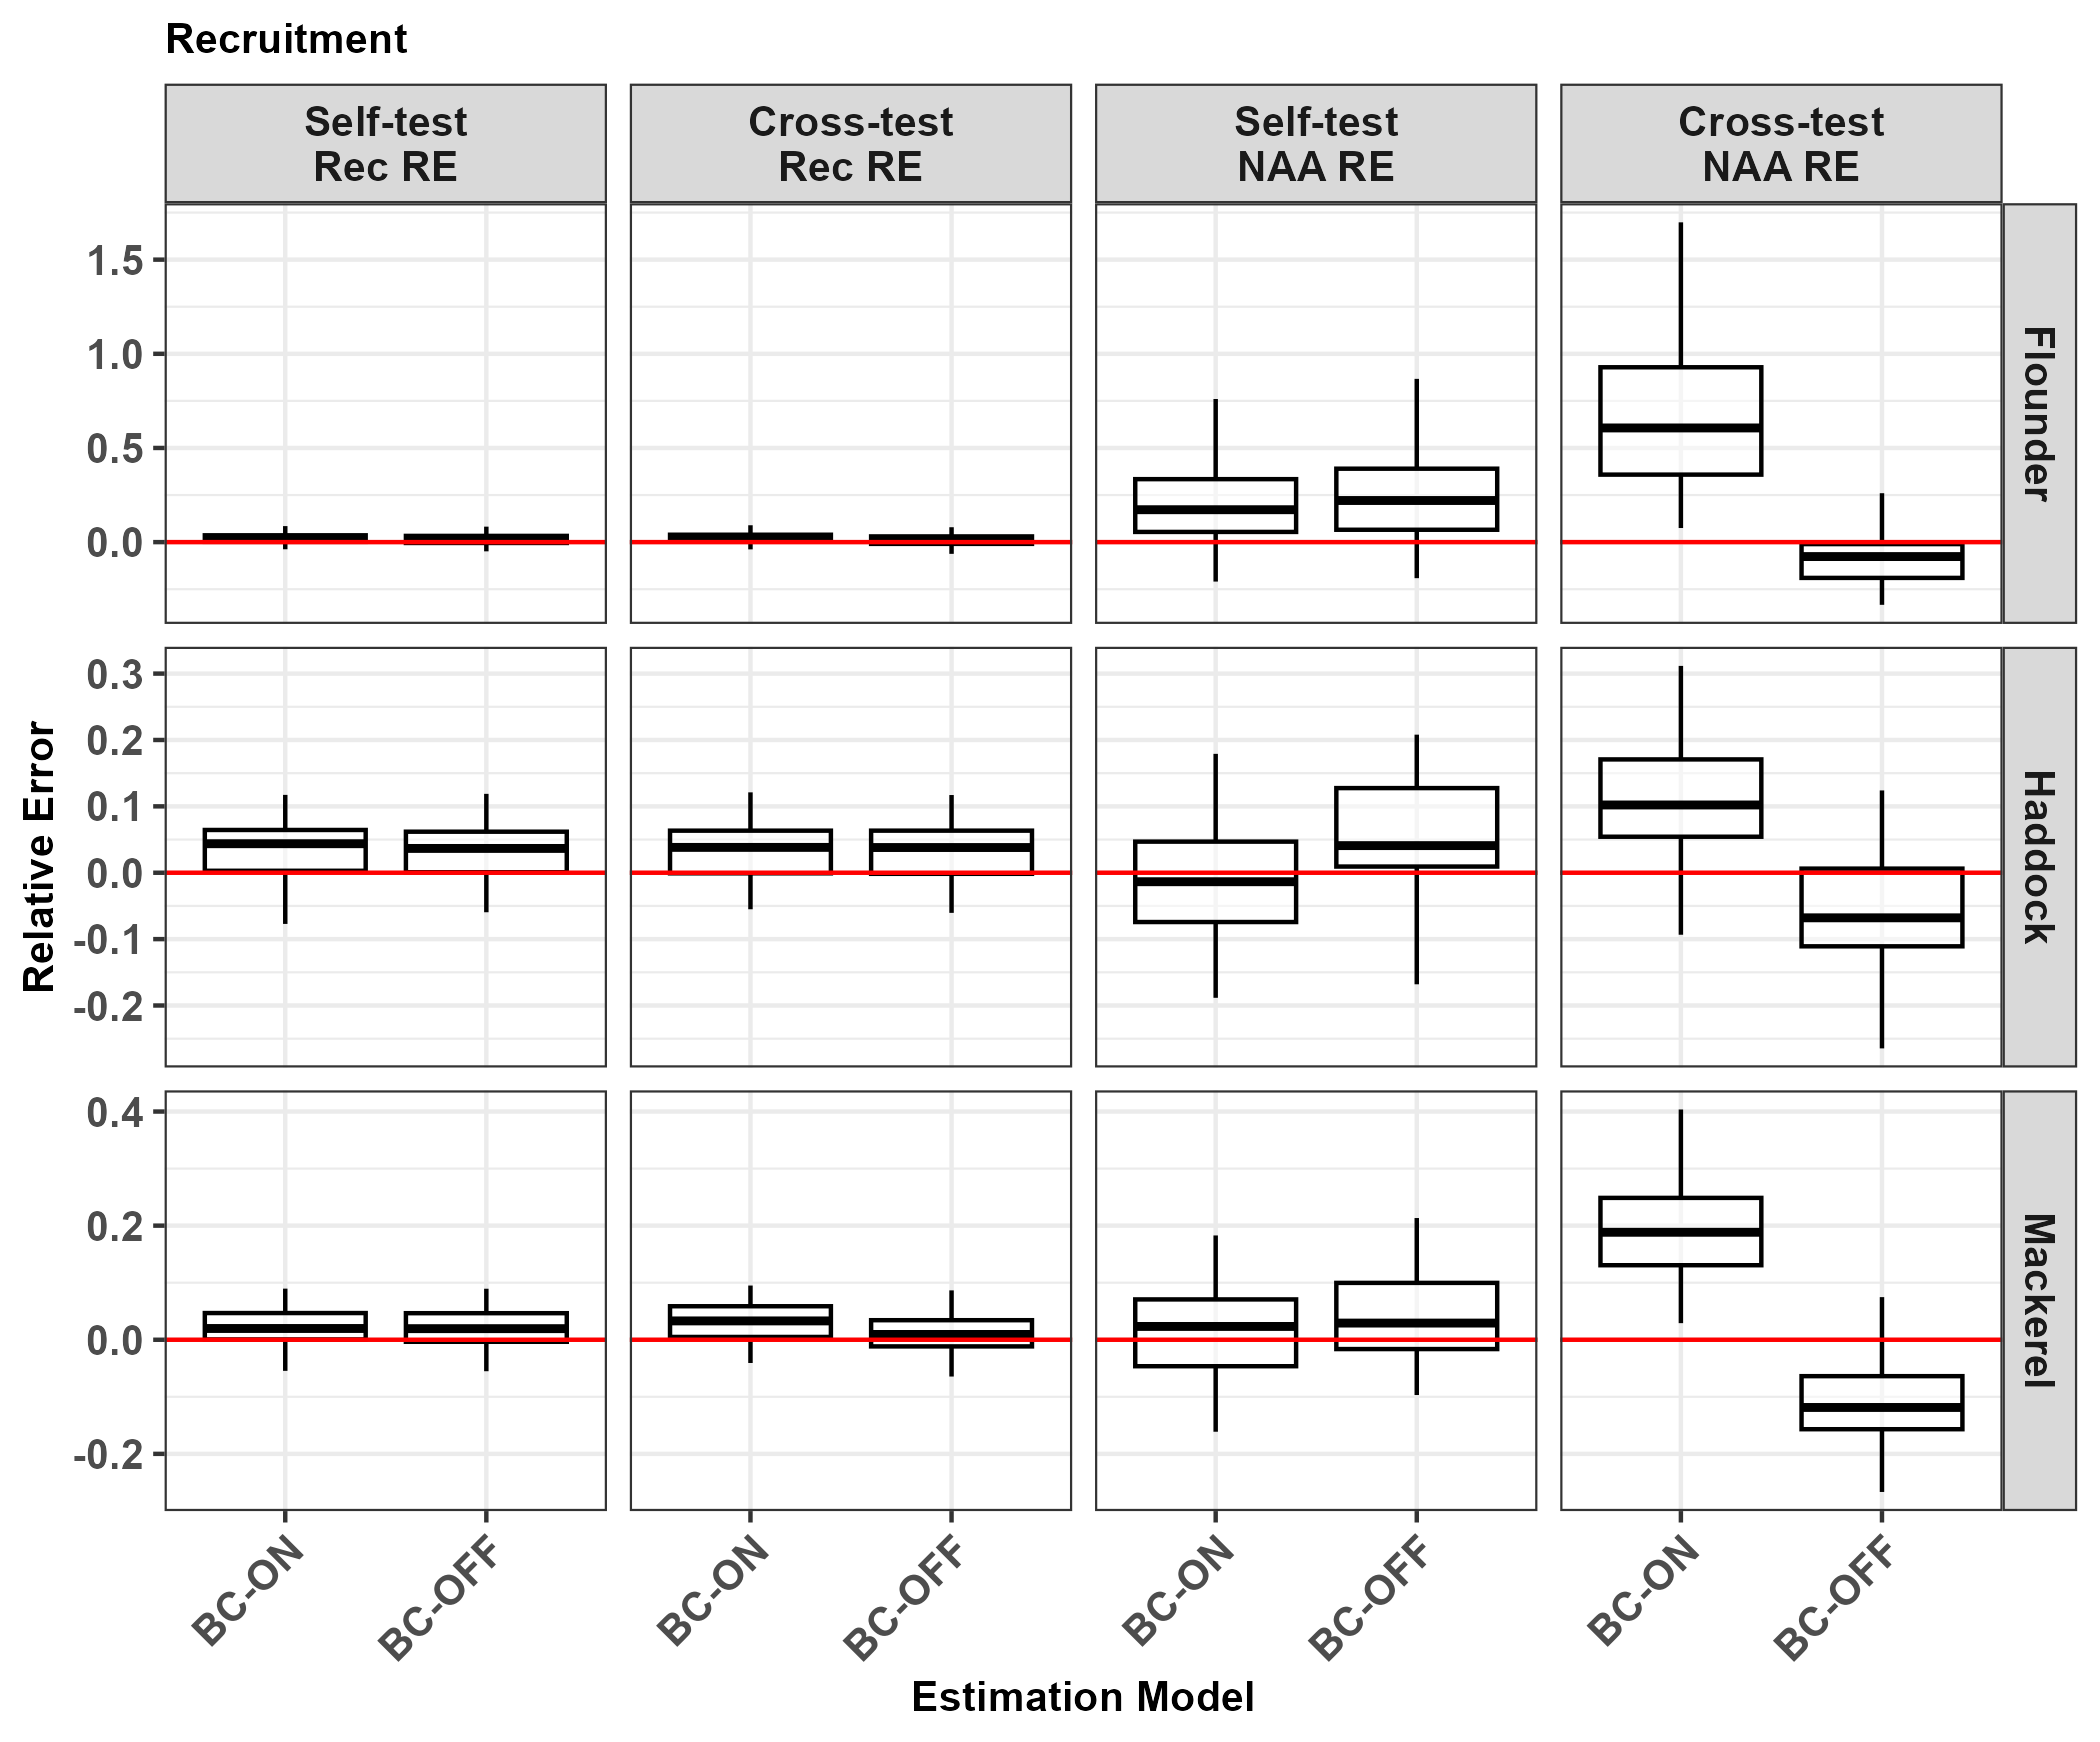
\includegraphics[width=\textwidth]{Original_Figures&Tables/Median_Rec.PNG}
\caption{Median relative error of reccruitment calculated for self-tests and cross-tests. "Rec RE" and "Rec+NAA RE" in the top facet indicate operating models (OMs) with only recruitment random effects and both recruitment and $NAA$ random effects, respectively.}
\label{fig:Median_Rec}
\end{figure}

\begin{figure}[H]
\centering
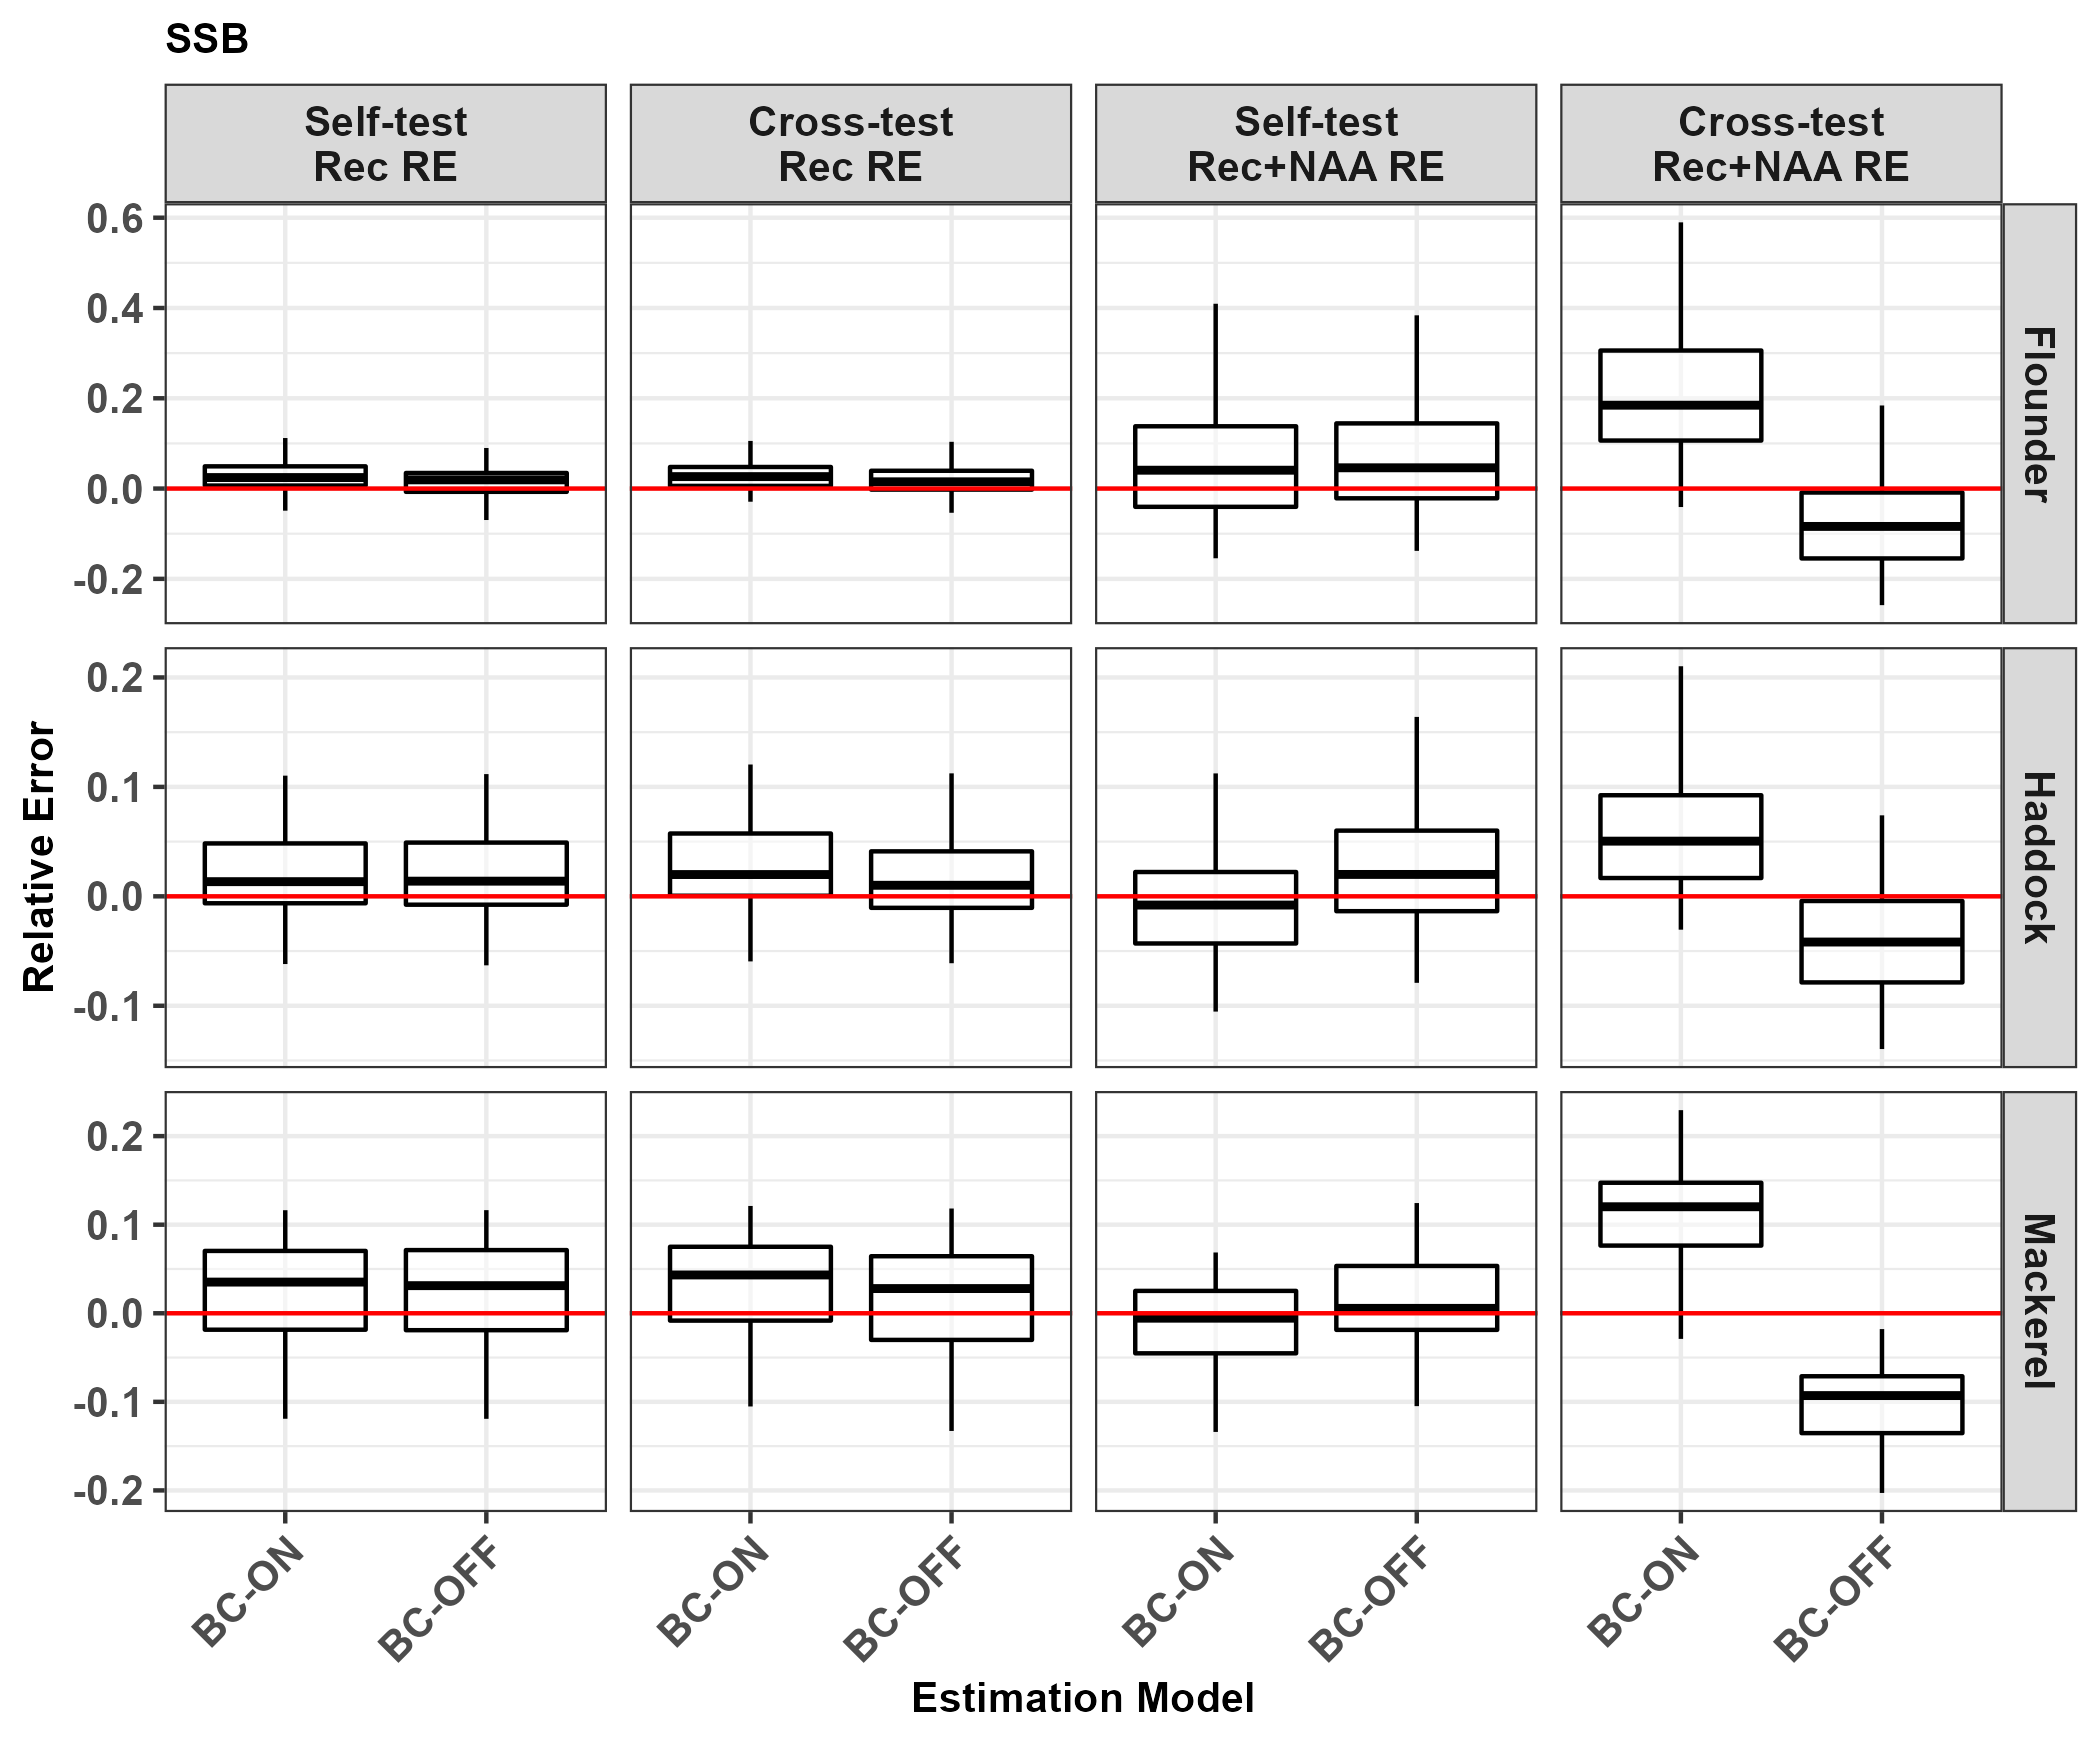
\includegraphics[width=\textwidth]{Original_Figures&Tables/Median_SSB.PNG}
\caption{Median relative error of $SSB$ calculated for self-tests and cross-tests. "Rec RE" and "Rec+NAA RE" in the top facet indicate operating models (OMs) with only recruitment random effects and both recruitment and $NAA$ random effects, respectively.}
\label{fig:Median_SSB}
\end{figure}

\begin{figure}[H]
\centering
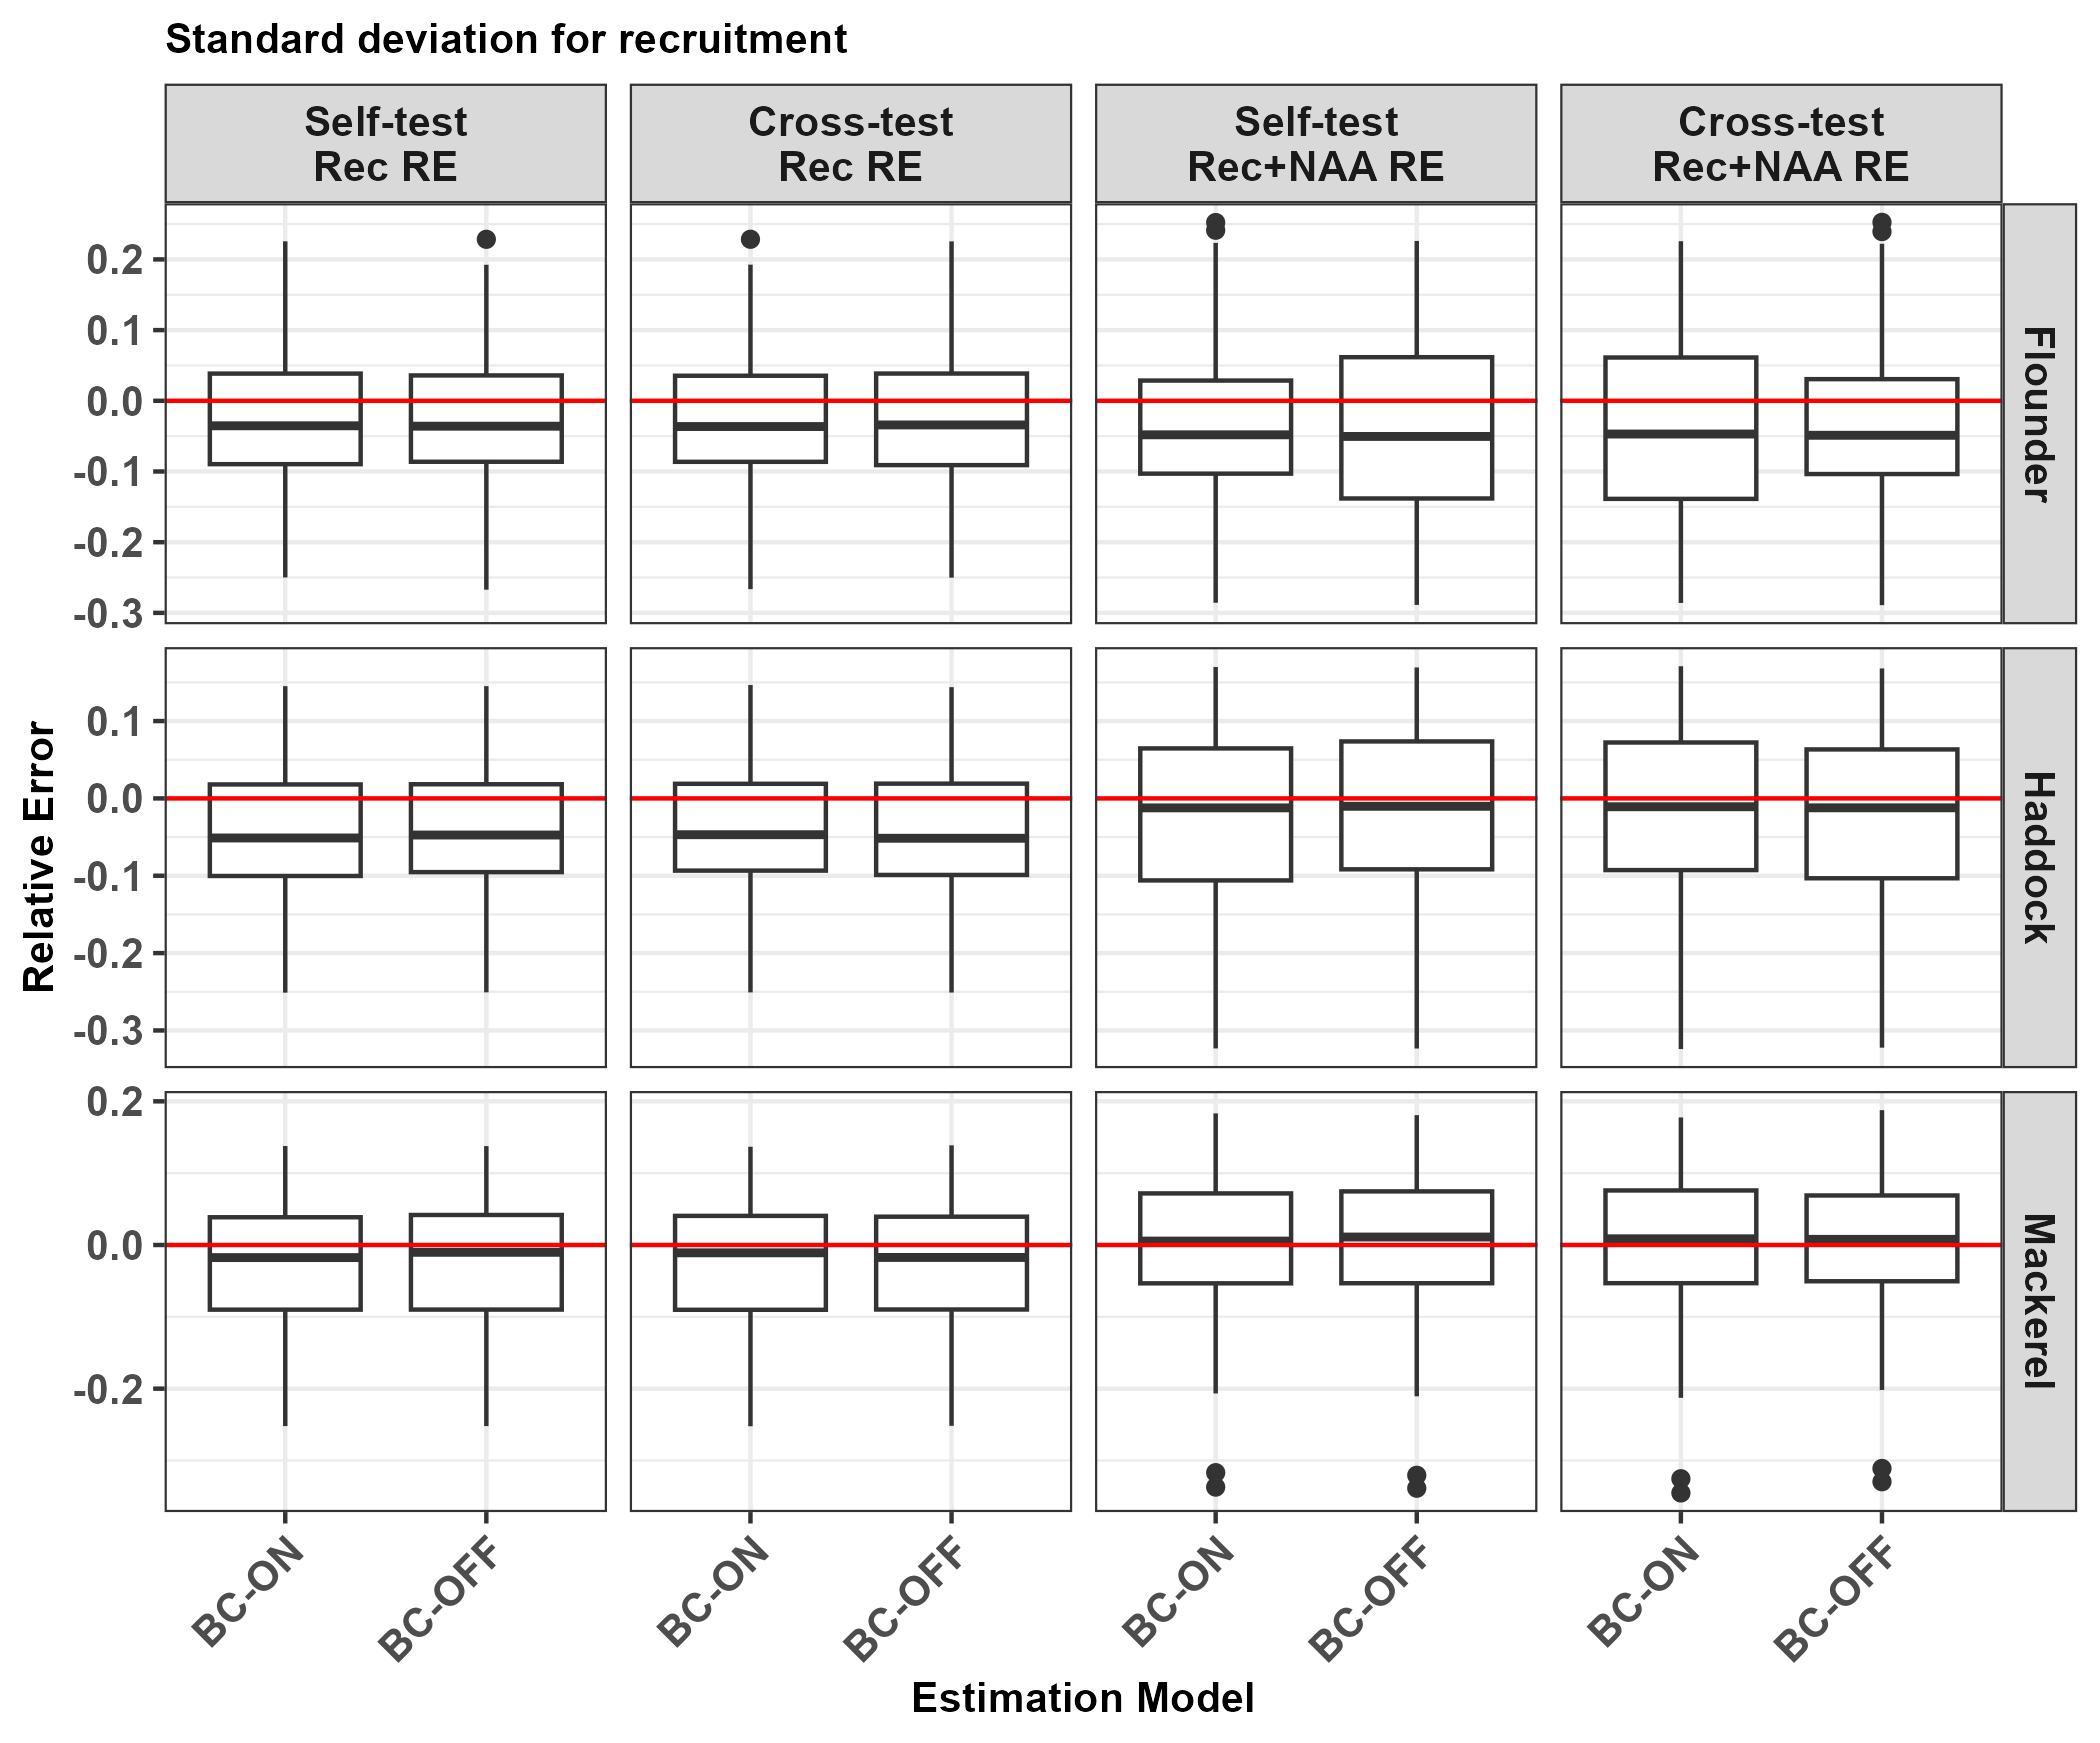
\includegraphics[width=\textwidth]{Original_Figures&Tables/Rec_sigma.PNG}
\caption{Relative error of recruitment variance calculated for self-tests and cross-tests. "Rec RE" and "Rec+NAA RE" in the top facet indicate operating models (OMs) with only recruitment random effects and both recruitment and $NAA$ random effects, respectively.}
\label{fig:Rec_sigma}
\end{figure}

\begin{figure}[H]
\centering
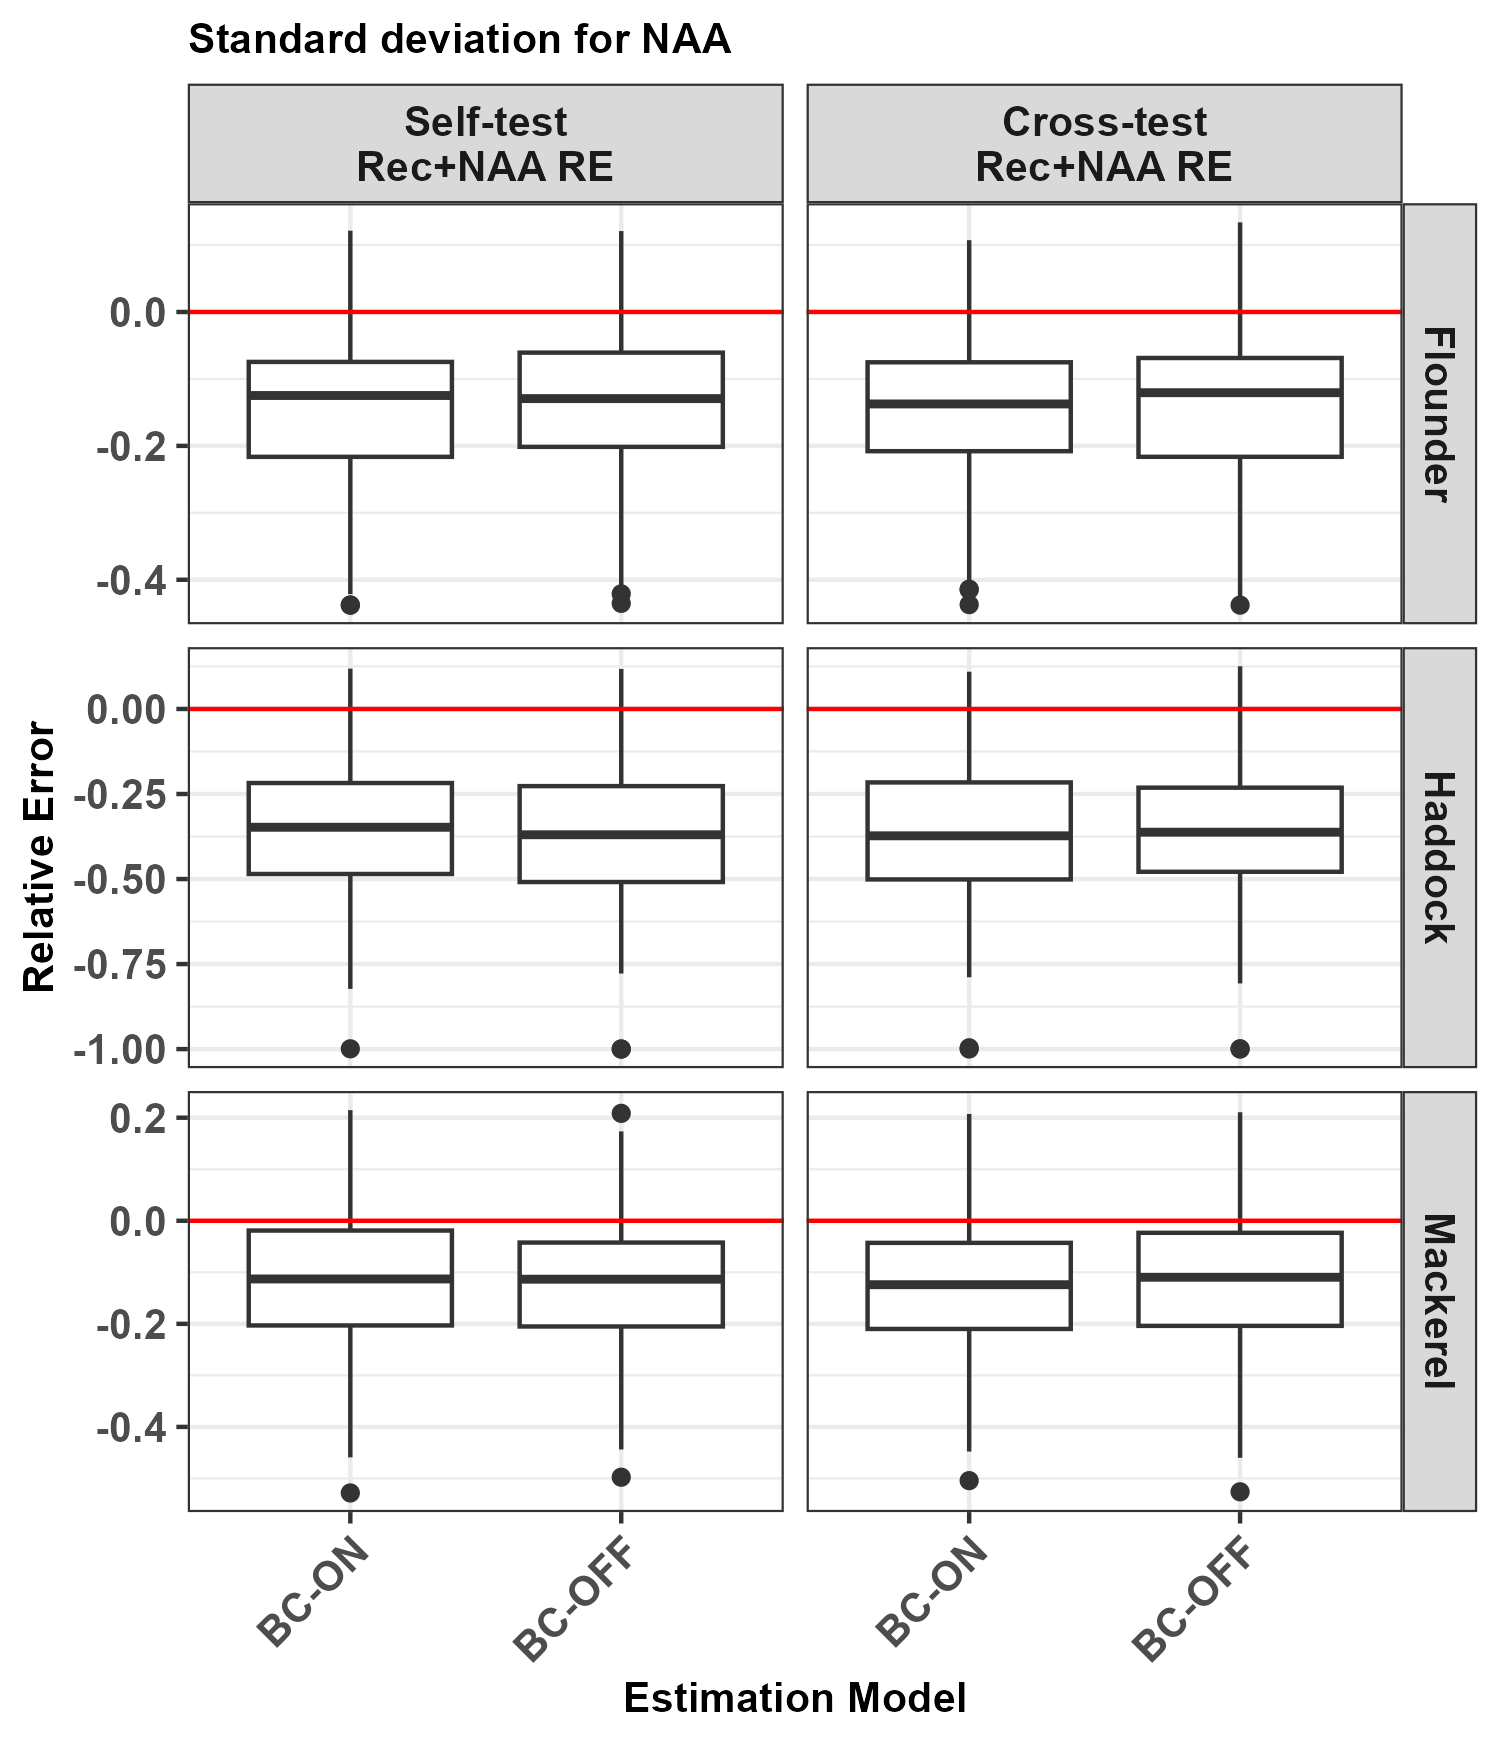
\includegraphics[width=\textwidth]{Original_Figures&Tables/NAA_sigma.PNG}
\caption{Relative error of $NAA$ variance calculated for self-tests and cross-tests. "Rec RE" and "Rec+NAA RE" in the top facet indicate operating models (OMs) with only recruitment random effects and both recruitment and $NAA$ random effects, respectively.}
\label{fig:NAA_sigma}
\end{figure}

\begin{figure}[H]
\centering
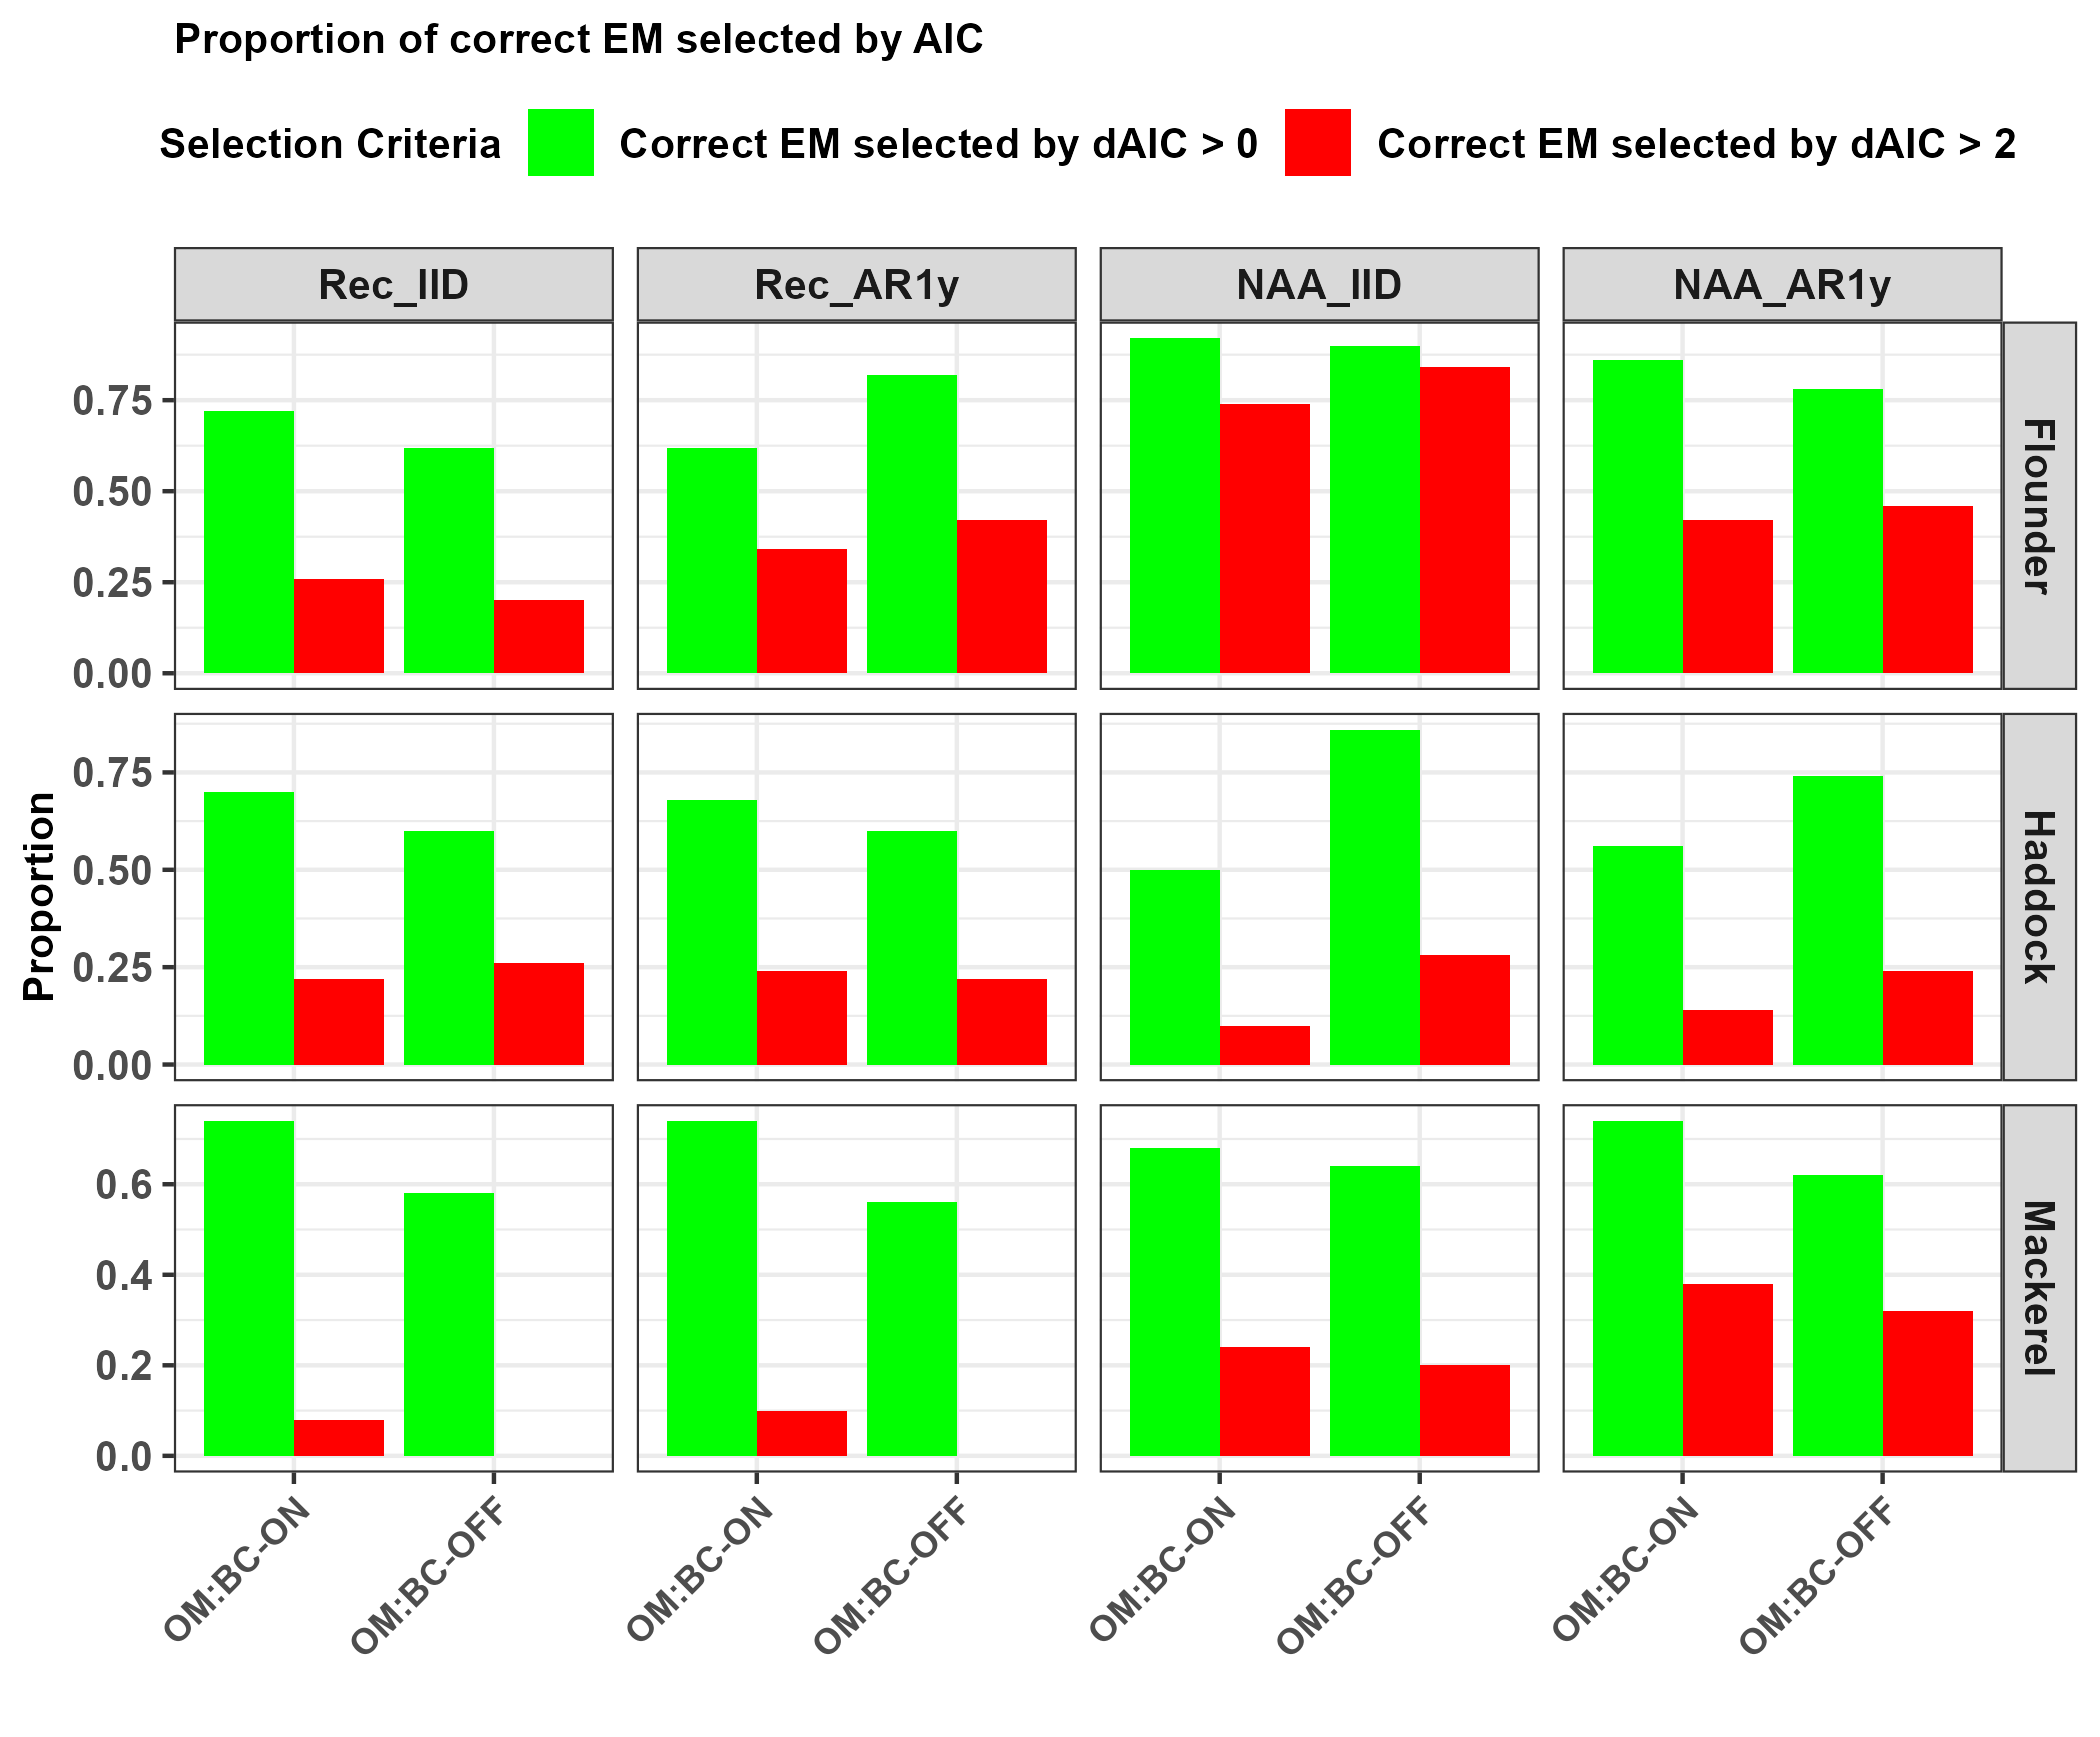
\includegraphics[width=\textwidth]{Original_Figures&Tables/AIC_select.PNG}
\caption{Probability of AIC selecting the correct estimation model (EM). The green color represents the proportion of the correct EM selected based on the lowest AIC, while the red color represents the proportion of the correct EM selected when the difference in AIC (dAIC) is greater than 2. The top facet displays operating models (OMs) with different forms of random-effects processes.}
\label{fig:AIC_select}
\end{figure}

\section{Supplementary files}\label{supplementary-files}

\renewcommand{\thetable}{S\arabic{table}}
\setcounter{table}{0}

\begin{table}[H]
    \centering
    \caption{Parameters associated with random effects processes used for Georges Bank (GB) yellowtail flounder.}
    \label{supp_flounder_table}
    \begin{table}[H]
    \centering
    \begin{tabular}{llrll}
        \toprule
        OM Structure & Proc./Obs. & Rec sigma & NAA sigma & Rho (AR1\_y) \\
        \midrule
        Rec (iid)       & ON \& ON   & 1.07 & NA & NA \\
        Rec (iid)       & OFF \& ON  & 1.07 & NA & NA \\
        Rec (iid)       & ON \& OFF  & 1.08 & NA & NA \\
        Rec (iid)       & OFF \& OFF & 1.08 & NA & NA \\
        Rec (ar1\_y)    & ON \& ON   & 0.37 & NA & 0.96 \\
        Rec (ar1\_y)    & OFF \& ON  & 0.37 & NA & 0.96 \\
        Rec (ar1\_y)    & ON \& OFF  & 0.37 & NA & 0.96 \\
        Rec (ar1\_y)    & OFF \& OFF & 0.37 & NA & 0.96 \\
        Rec+NAA (iid)      & ON \& ON   & 1.23 & 0.55 & NA \\
        Rec+NAA (iid)      & OFF \& ON  & 1.23 & 0.56 & NA \\
        Rec+NAA (iid)      & ON \& OFF  & 1.24 & 0.55 & NA \\
        Rec+NAA (iid)      & OFF \& OFF & 1.24 & 0.56 & NA \\
        Rec+NAA (ar1\_y)   & ON \& ON   & 0.55 & 0.21 & 0.94 \\
        Rec+NAA (ar1\_y)   & OFF \& ON  & 0.55 & 0.21 & 0.94 \\
        Rec+NAA (ar1\_y)   & ON \& OFF  & 0.55 & 0.21 & 0.94 \\
        Rec+NAA (ar1\_y)   & OFF \& OFF & 0.55 & 0.21 & 0.94 \\
        \bottomrule
    \end{tabular}
\end{table}

\end{table}

\begin{table}[H]
    \centering
    \caption{Parameters associated with random effects processes used for Gulf of Maine (GoM) haddock.}
    \label{supp_haddock_table}
    \begin{table}[H]
    \centering
    \begin{tabular}{llrll}
        \toprule
         OM Structure & Proc./Obs. & Rec sigma & NAA sigma & Rho (AR1\_y) \\
        \midrule
        Rec (iid)       & ON \& ON   & 1.57 & NA & NA \\
        Rec (iid)       & OFF \& ON  & 1.57 & NA & NA \\
        Rec (iid)       & ON \& OFF  & 1.59 & NA & NA \\
        Rec (iid)       & OFF \& OFF & 1.59 & NA & NA \\
        Rec (ar1\_y)    & ON \& ON   & 1.16 & NA & 0.7 \\
        Rec (ar1\_y)    & OFF \& ON  & 1.16 & NA & 0.7 \\
        Rec (ar1\_y)    & ON \& OFF  & 1.17 & NA & 0.71 \\
        Rec (ar1\_y)    & OFF \& OFF & 1.17 & NA & 0.71 \\
        Rec+NAA (iid)     & ON \& ON   & 1.60 & 0.2 & NA \\
        Rec+NAA (iid)     & OFF \& ON  & 1.60 & 0.2 & NA \\
        Rec+NAA (iid)     & ON \& OFF  & 1.62 & 0.2 & NA \\
        Rec+NAA (iid)     & OFF \& OFF & 1.62 & 0.2 & NA \\
        Rec+NAA (ar1\_y)  & ON \& ON   & 1.18 & 0.16 & 0.6 \\
        Rec+NAA (ar1\_y)  & OFF \& ON  & 1.18 & 0.16 & 0.6 \\
        Rec+NAA (ar1\_y)  & ON \& OFF  & 1.18 & 0.17 & 0.61 \\
        Rec+NAA (ar1\_y)  & OFF \& OFF & 1.18 & 0.16 & 0.61 \\
        \bottomrule
    \end{tabular}
\end{table}

\end{table}

\begin{table}[H]
    \centering
    \caption{Parameters associated with random effects processes used for Atlantic mackerel.}
    \label{supp_mackerel_table}
    \begin{table}[H]
    \centering
    \begin{tabular}{llrll}
        \toprule
         OM Structure & Proc./Obs. & Rec sigma & NAA sigma & Rho (AR1\_y) \\
        \midrule
        Rec (iid)       & ON \& ON   & 1.11 & NA & NA \\
        Rec (iid)       & OFF \& ON  & 1.11 & NA & NA \\
        Rec (iid)       & ON \& OFF  & 1.11 & NA & NA \\
        Rec (iid)       & OFF \& OFF & 1.11 & NA & NA \\
        Rec (ar1\_y)    & ON \& ON   & 1.00 & NA & 0.46 \\
        Rec (ar1\_y)    & OFF \& ON  & 1.00 & NA & 0.46 \\
        Rec (ar1\_y)    & ON \& OFF  & 1.01 & NA & 0.46 \\
        Rec (ar1\_y)    & OFF \& OFF & 1.01 & NA & 0.46 \\
        Rec+NAA (iid)     & ON \& ON   & 1.02 & 0.28 & NA \\
        Rec+NAA (iid)     & OFF \& ON  & 1.02 & 0.28 & NA \\
        Rec+NAA (iid)     & ON \& OFF  & 1.02 & 0.28 & NA \\
        Rec+NAA (iid)     & OFF \& OFF & 1.02 & 0.28 & NA \\
        Rec+NAA (ar1\_y)  & ON \& ON   & 0.89 & 0.32 & 0.49 \\
        Rec+NAA (ar1\_y)  & OFF \& ON  & 0.89 & 0.32 & 0.49 \\
        Rec+NAA (ar1\_y)  & ON \& OFF  & 0.90 & 0.32 & 0.48 \\
        Rec+NAA (ar1\_y)  & OFF \& OFF & 0.90 & 0.32 & 0.48 \\
        \bottomrule
    \end{tabular}
\end{table}

\end{table}

\renewcommand{\thetable}{\arabic{table}}

\renewcommand{\thefigure}{S\arabic{figure}}
\setcounter{figure}{0}

\begin{figure}[H]
    \centering
    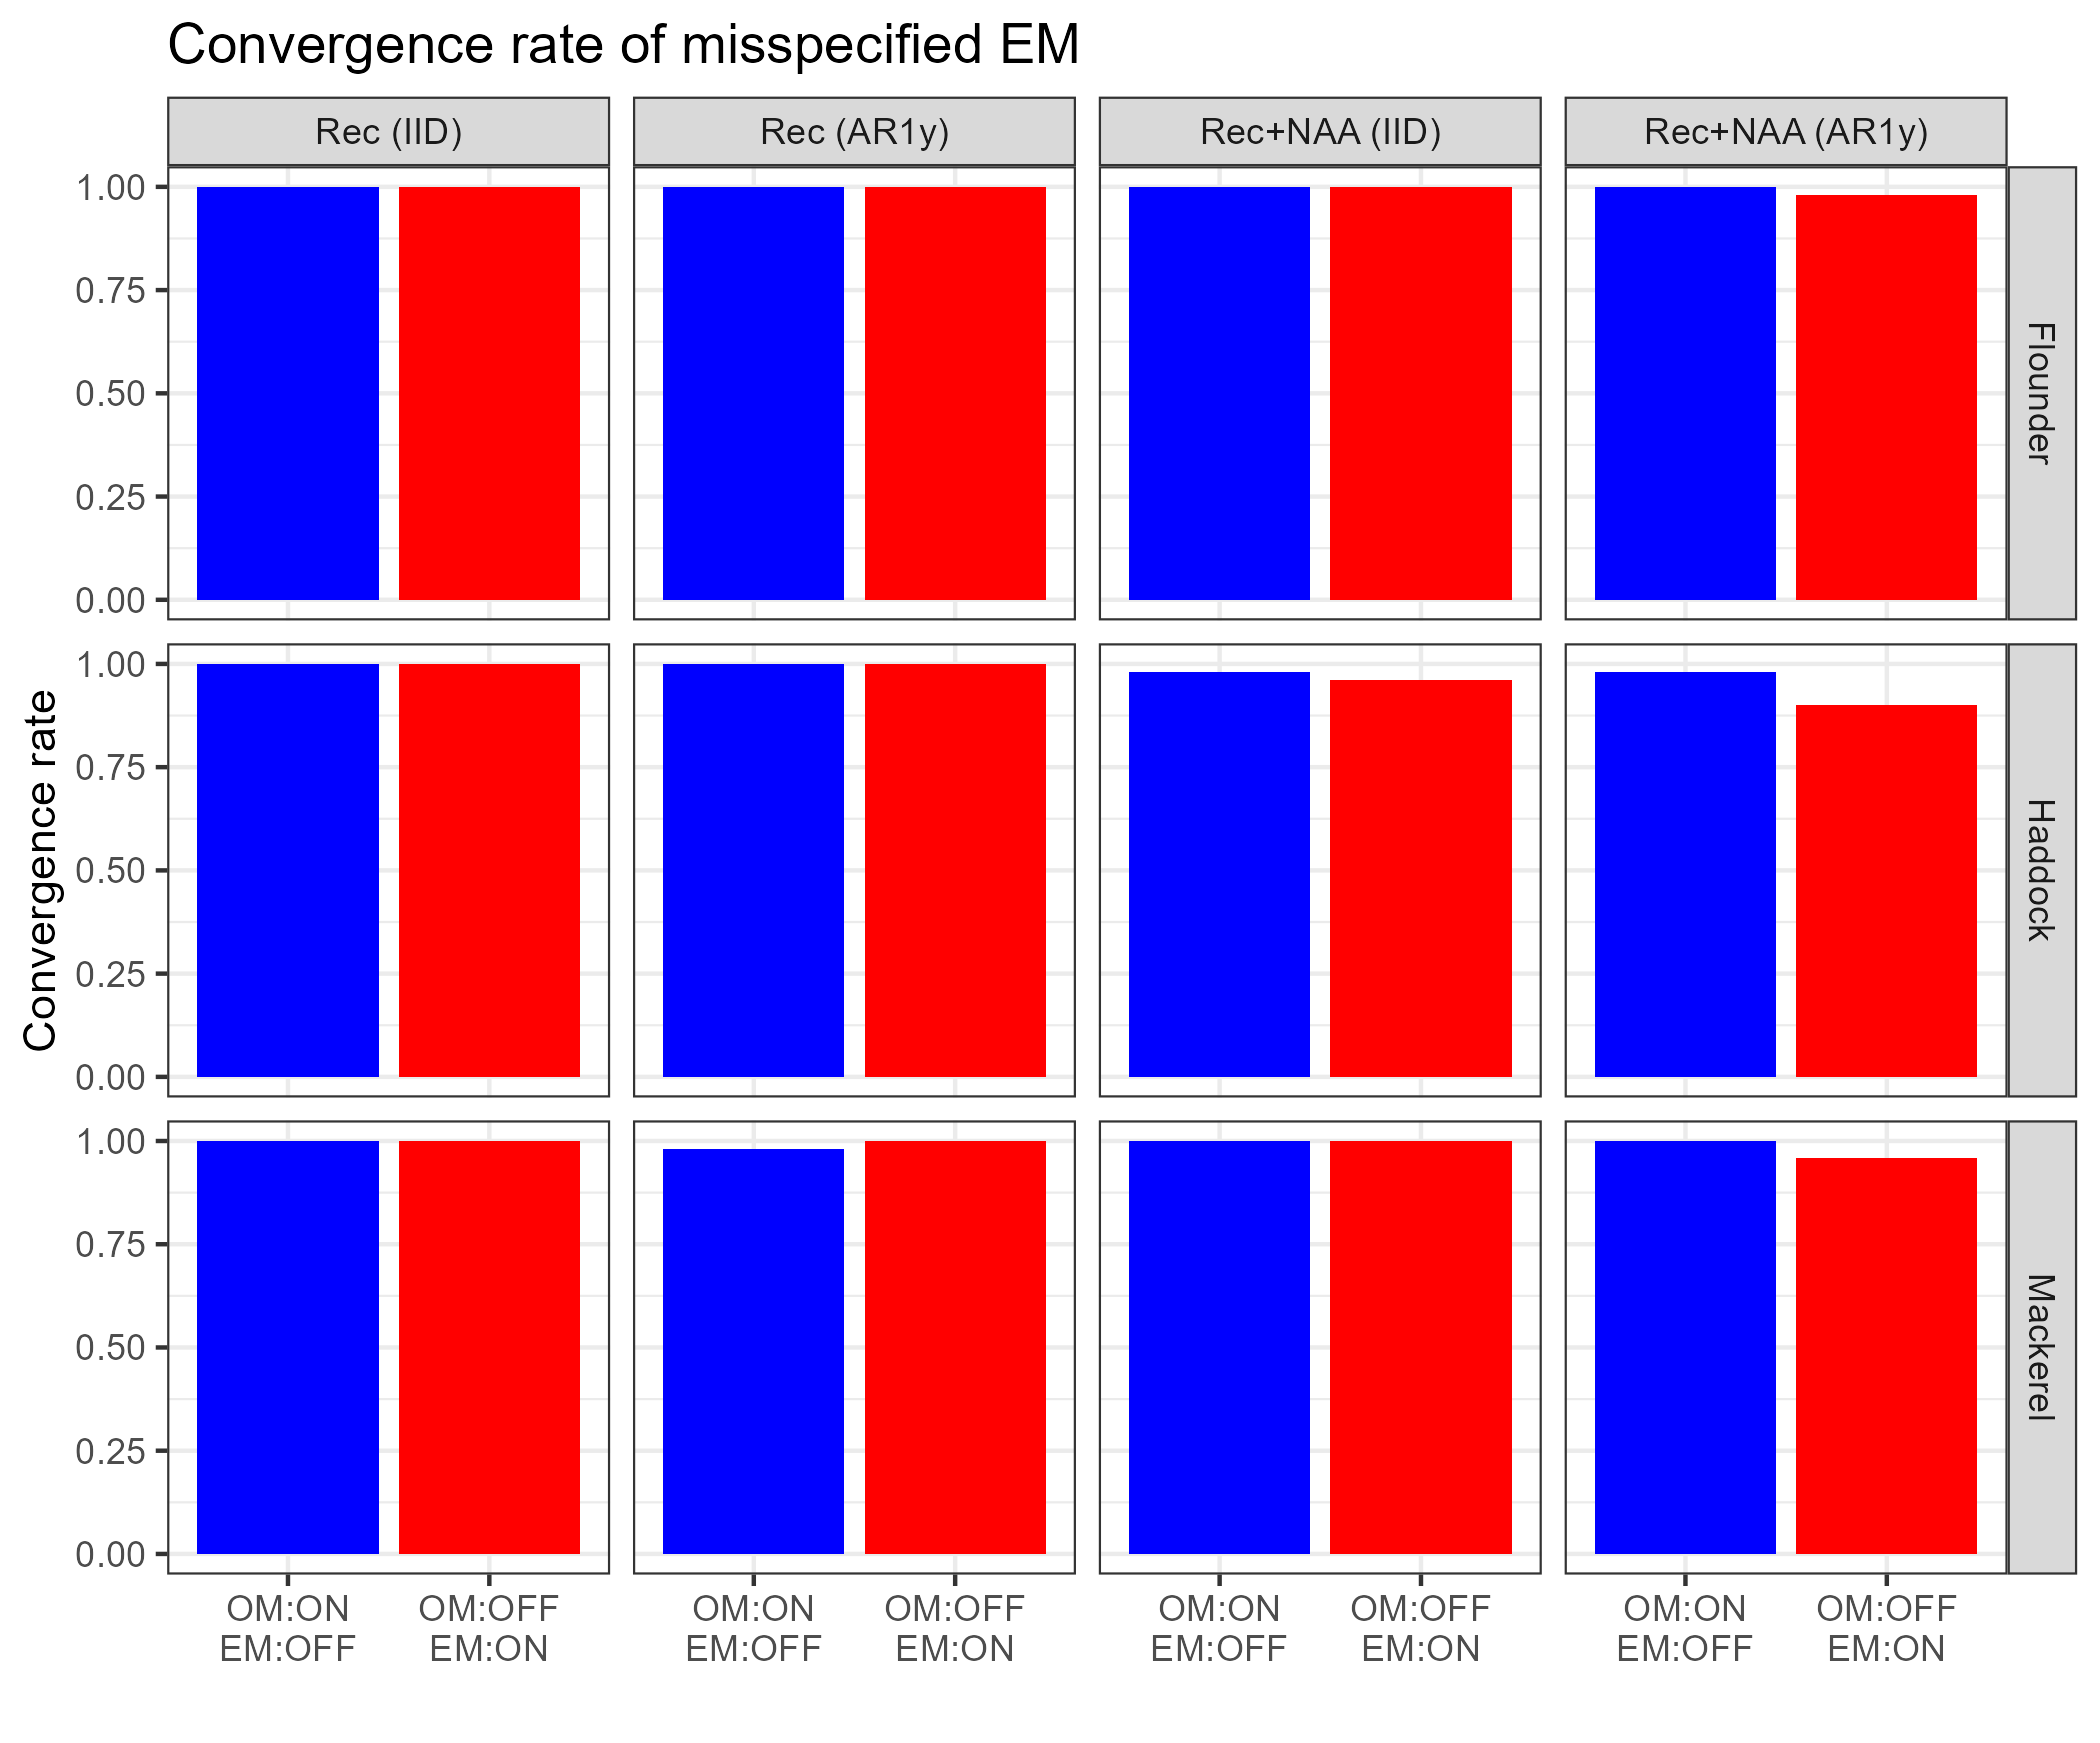
\includegraphics[width=\textwidth]{Original_Figures&Tables/Convergence.PNG}
    \caption{Convergence rate of the misspecified estimation model (EM) in cross-tests.}
    \label{fig:supp_conv}
\end{figure}

\begin{figure}[H]
    \centering
    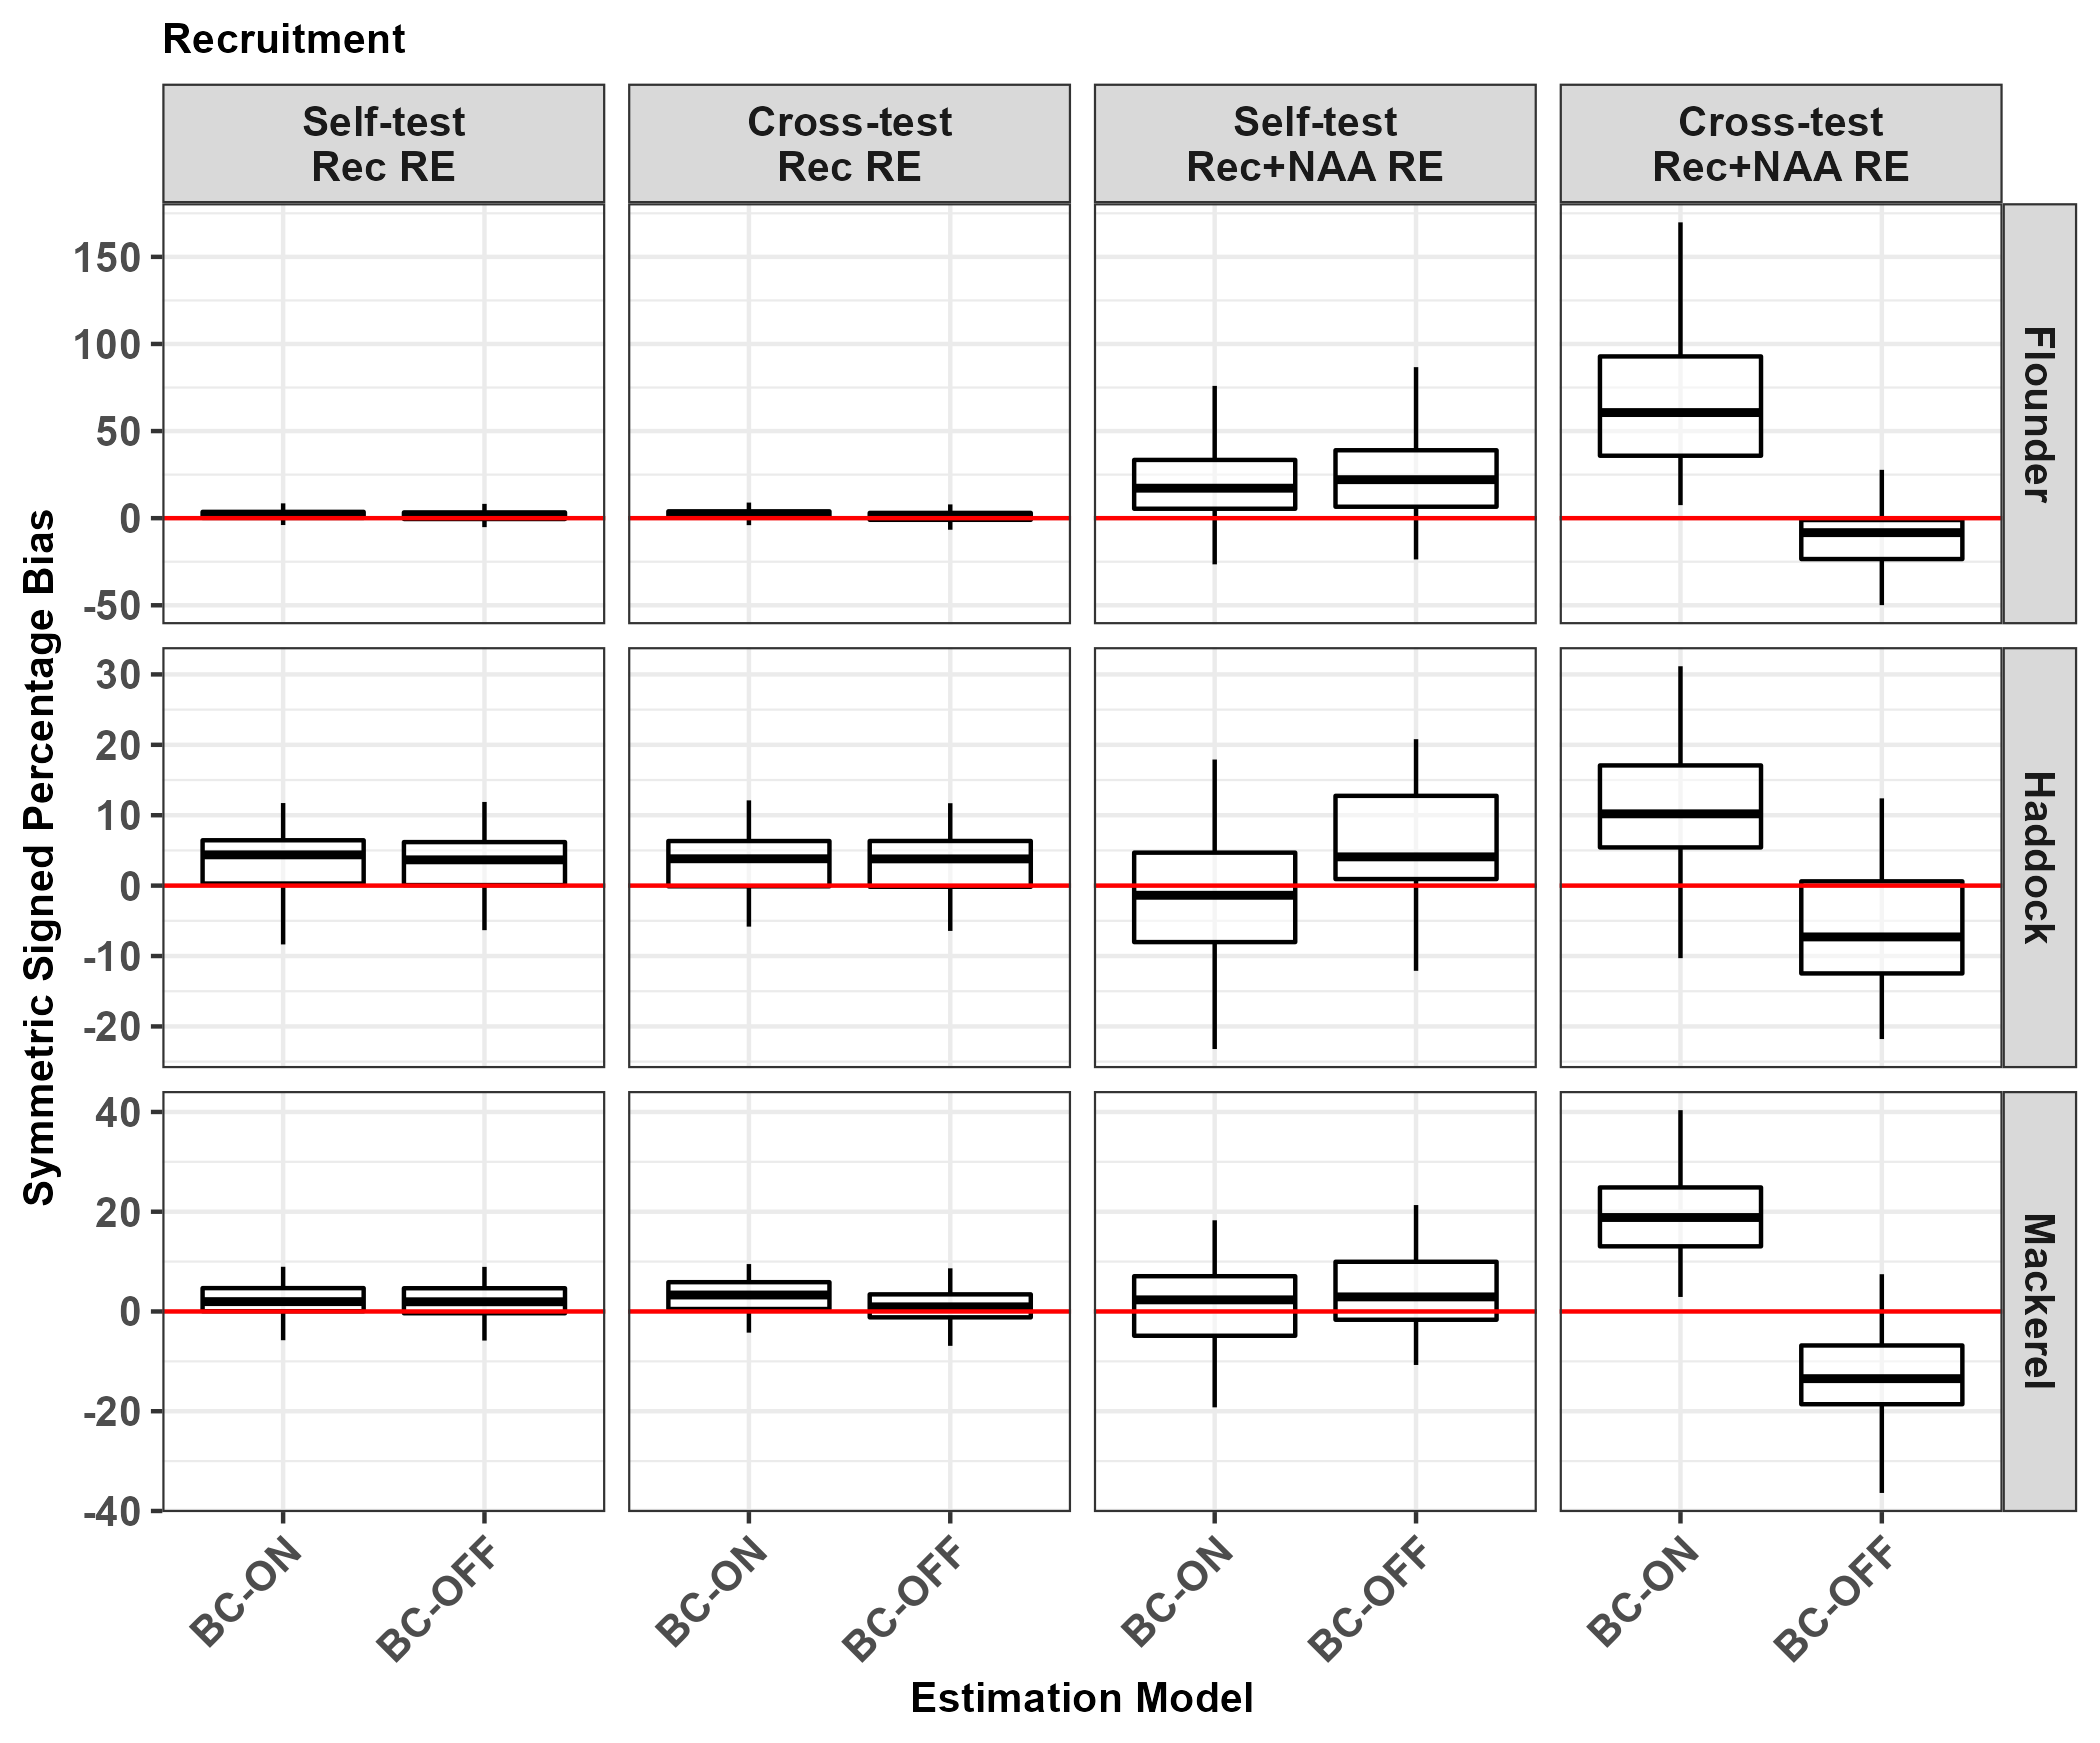
\includegraphics[width=\textwidth]{Original_Figures&Tables/Median_Rec_SSPB.PNG}
    \caption{Median symmetric signed percentage bias (SSPB) of recruitment calculated for self-tests and cross-tests. "Rec RE" and "Rec+NAA RE" in the top facet indicate operating models (OMs) with only recruitment random effects and both recruitment and $NAA$ random effects, respectively.}
    \label{fig:supp_Rec_SSPB}
\end{figure}

\begin{figure}[H]
    \centering
    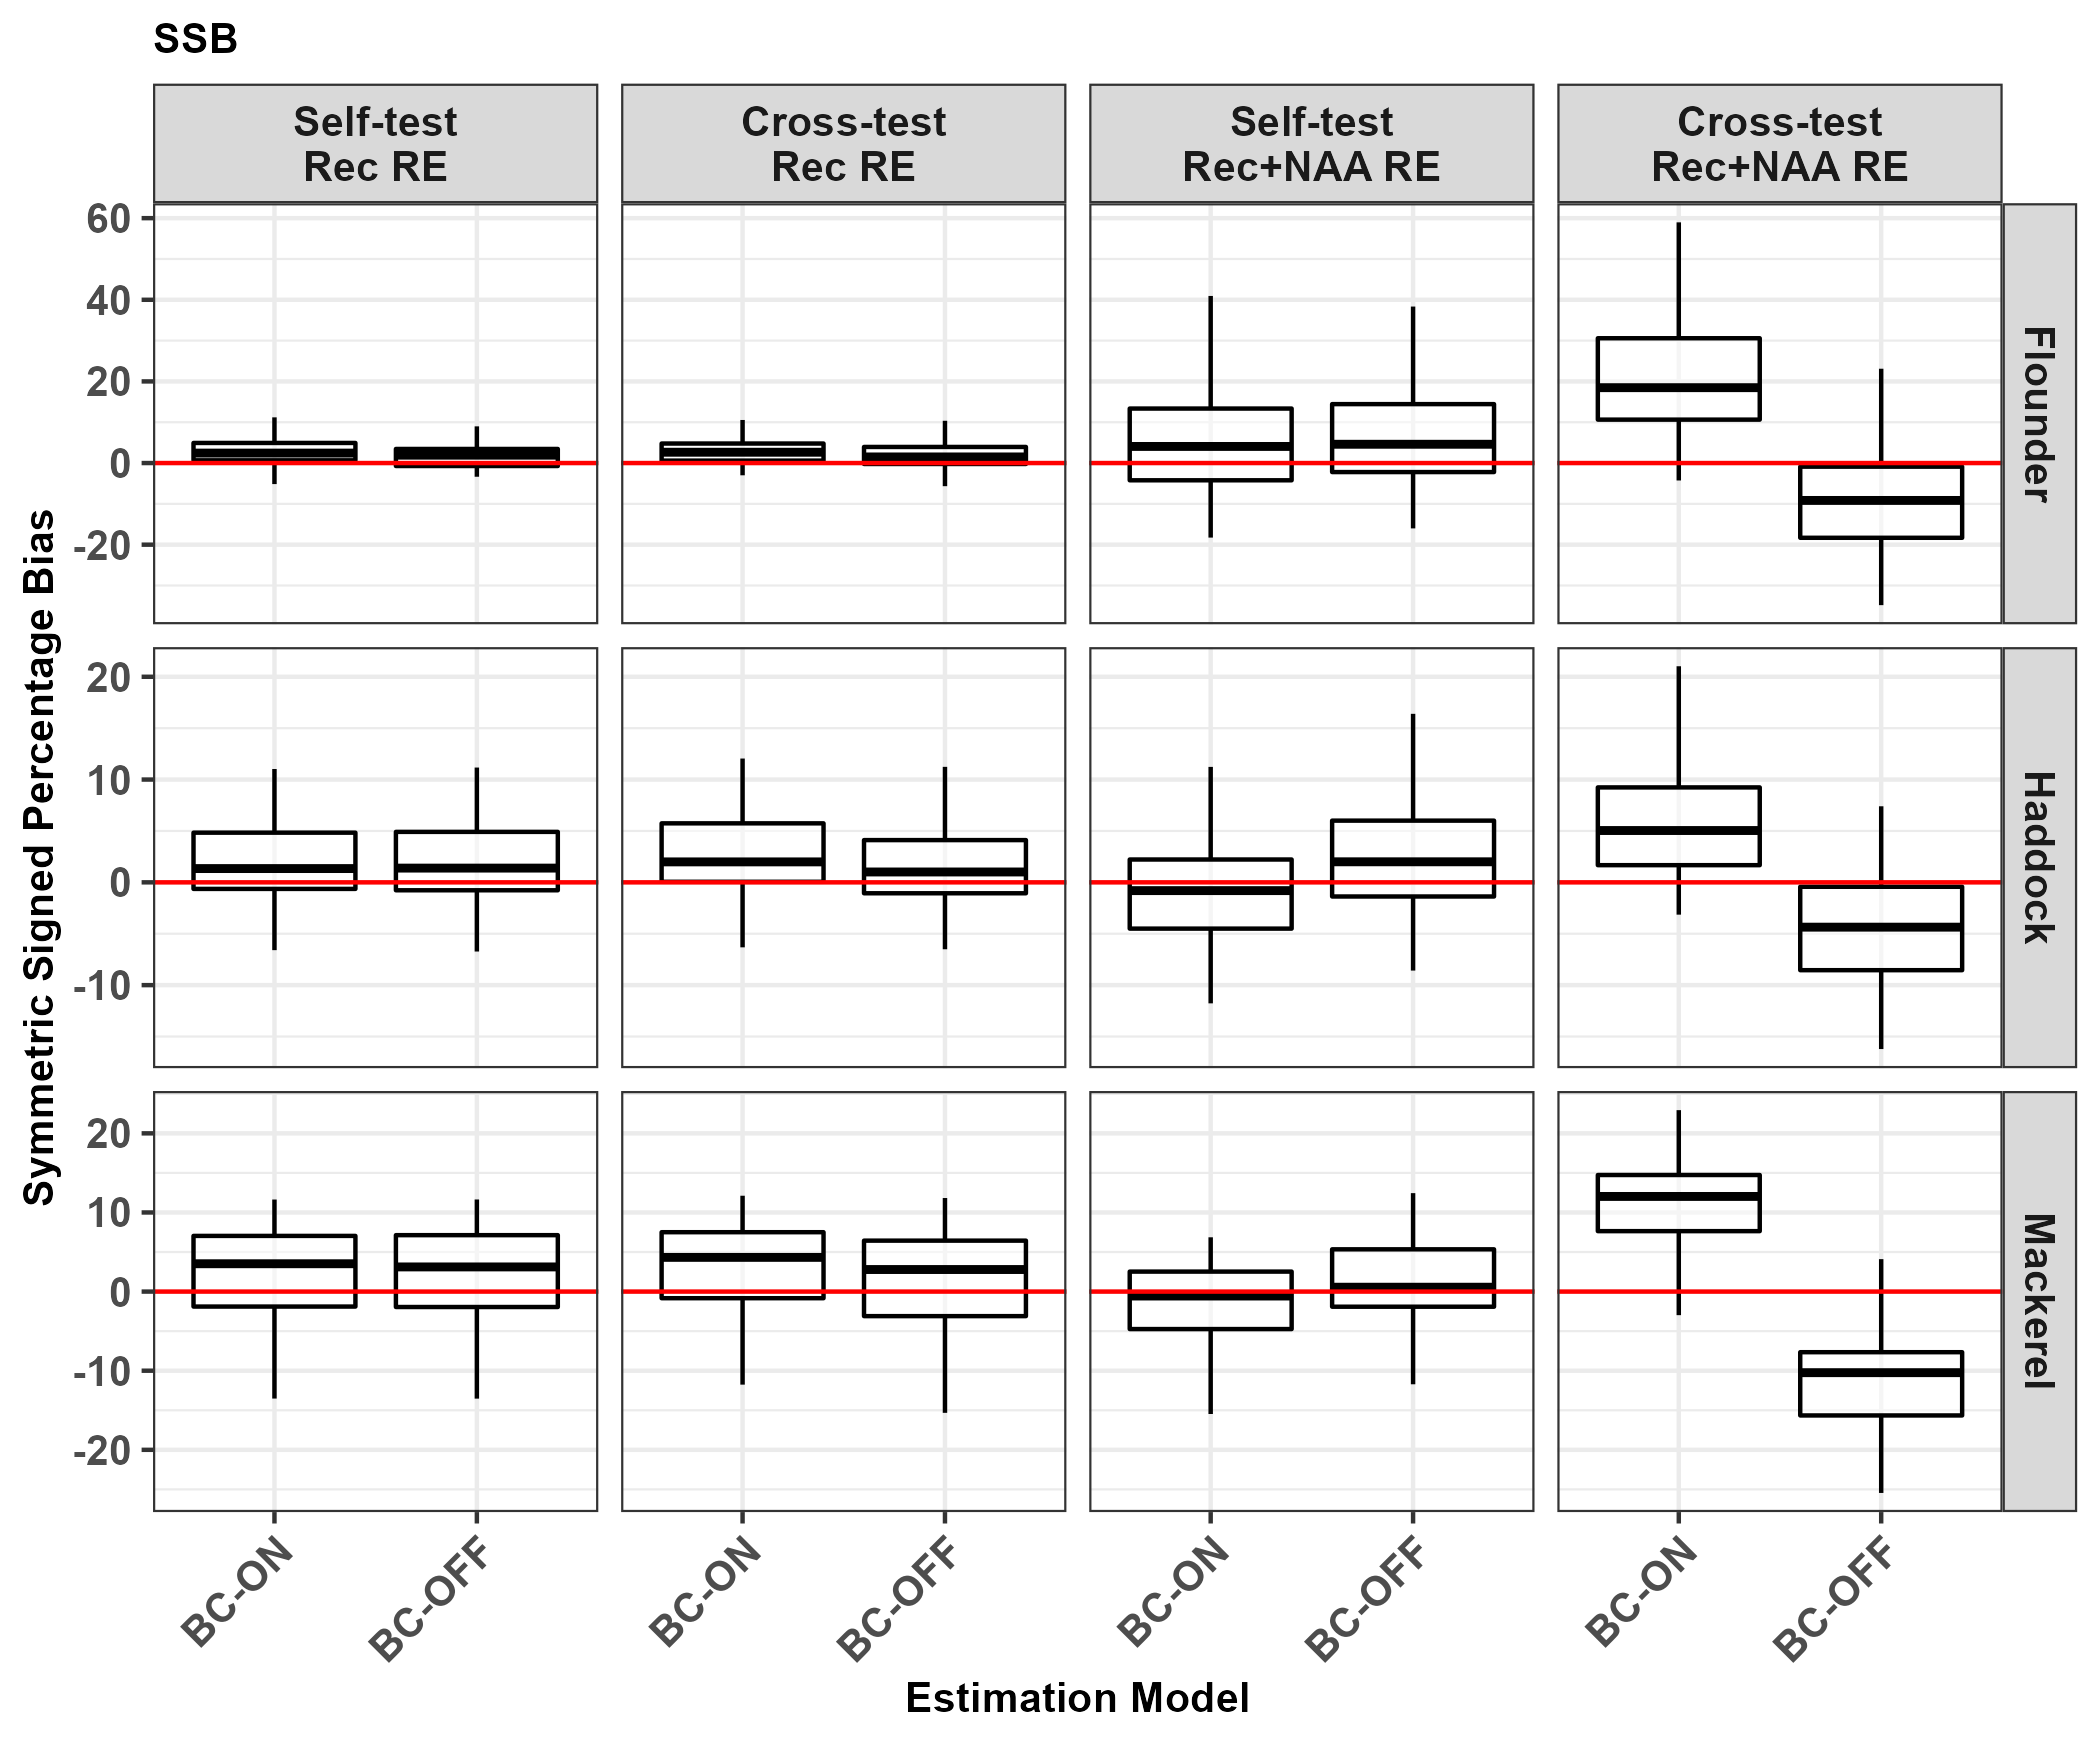
\includegraphics[width=\textwidth]{Original_Figures&Tables/Median_SSB_SSPB.PNG}
    \caption{Median symmetric signed percentage bias (SSPB) of $SSB$ calculated for self-tests and cross-tests. "Rec RE" and "Rec+NAA RE" in the top facet indicate operating models (OMs) with only recruitment random effects and both recruitment and $NAA$ random effects, respectively.}
    \label{fig:supp_SSB_SSPB}
\end{figure}

\begin{figure}[H]
    \centering
    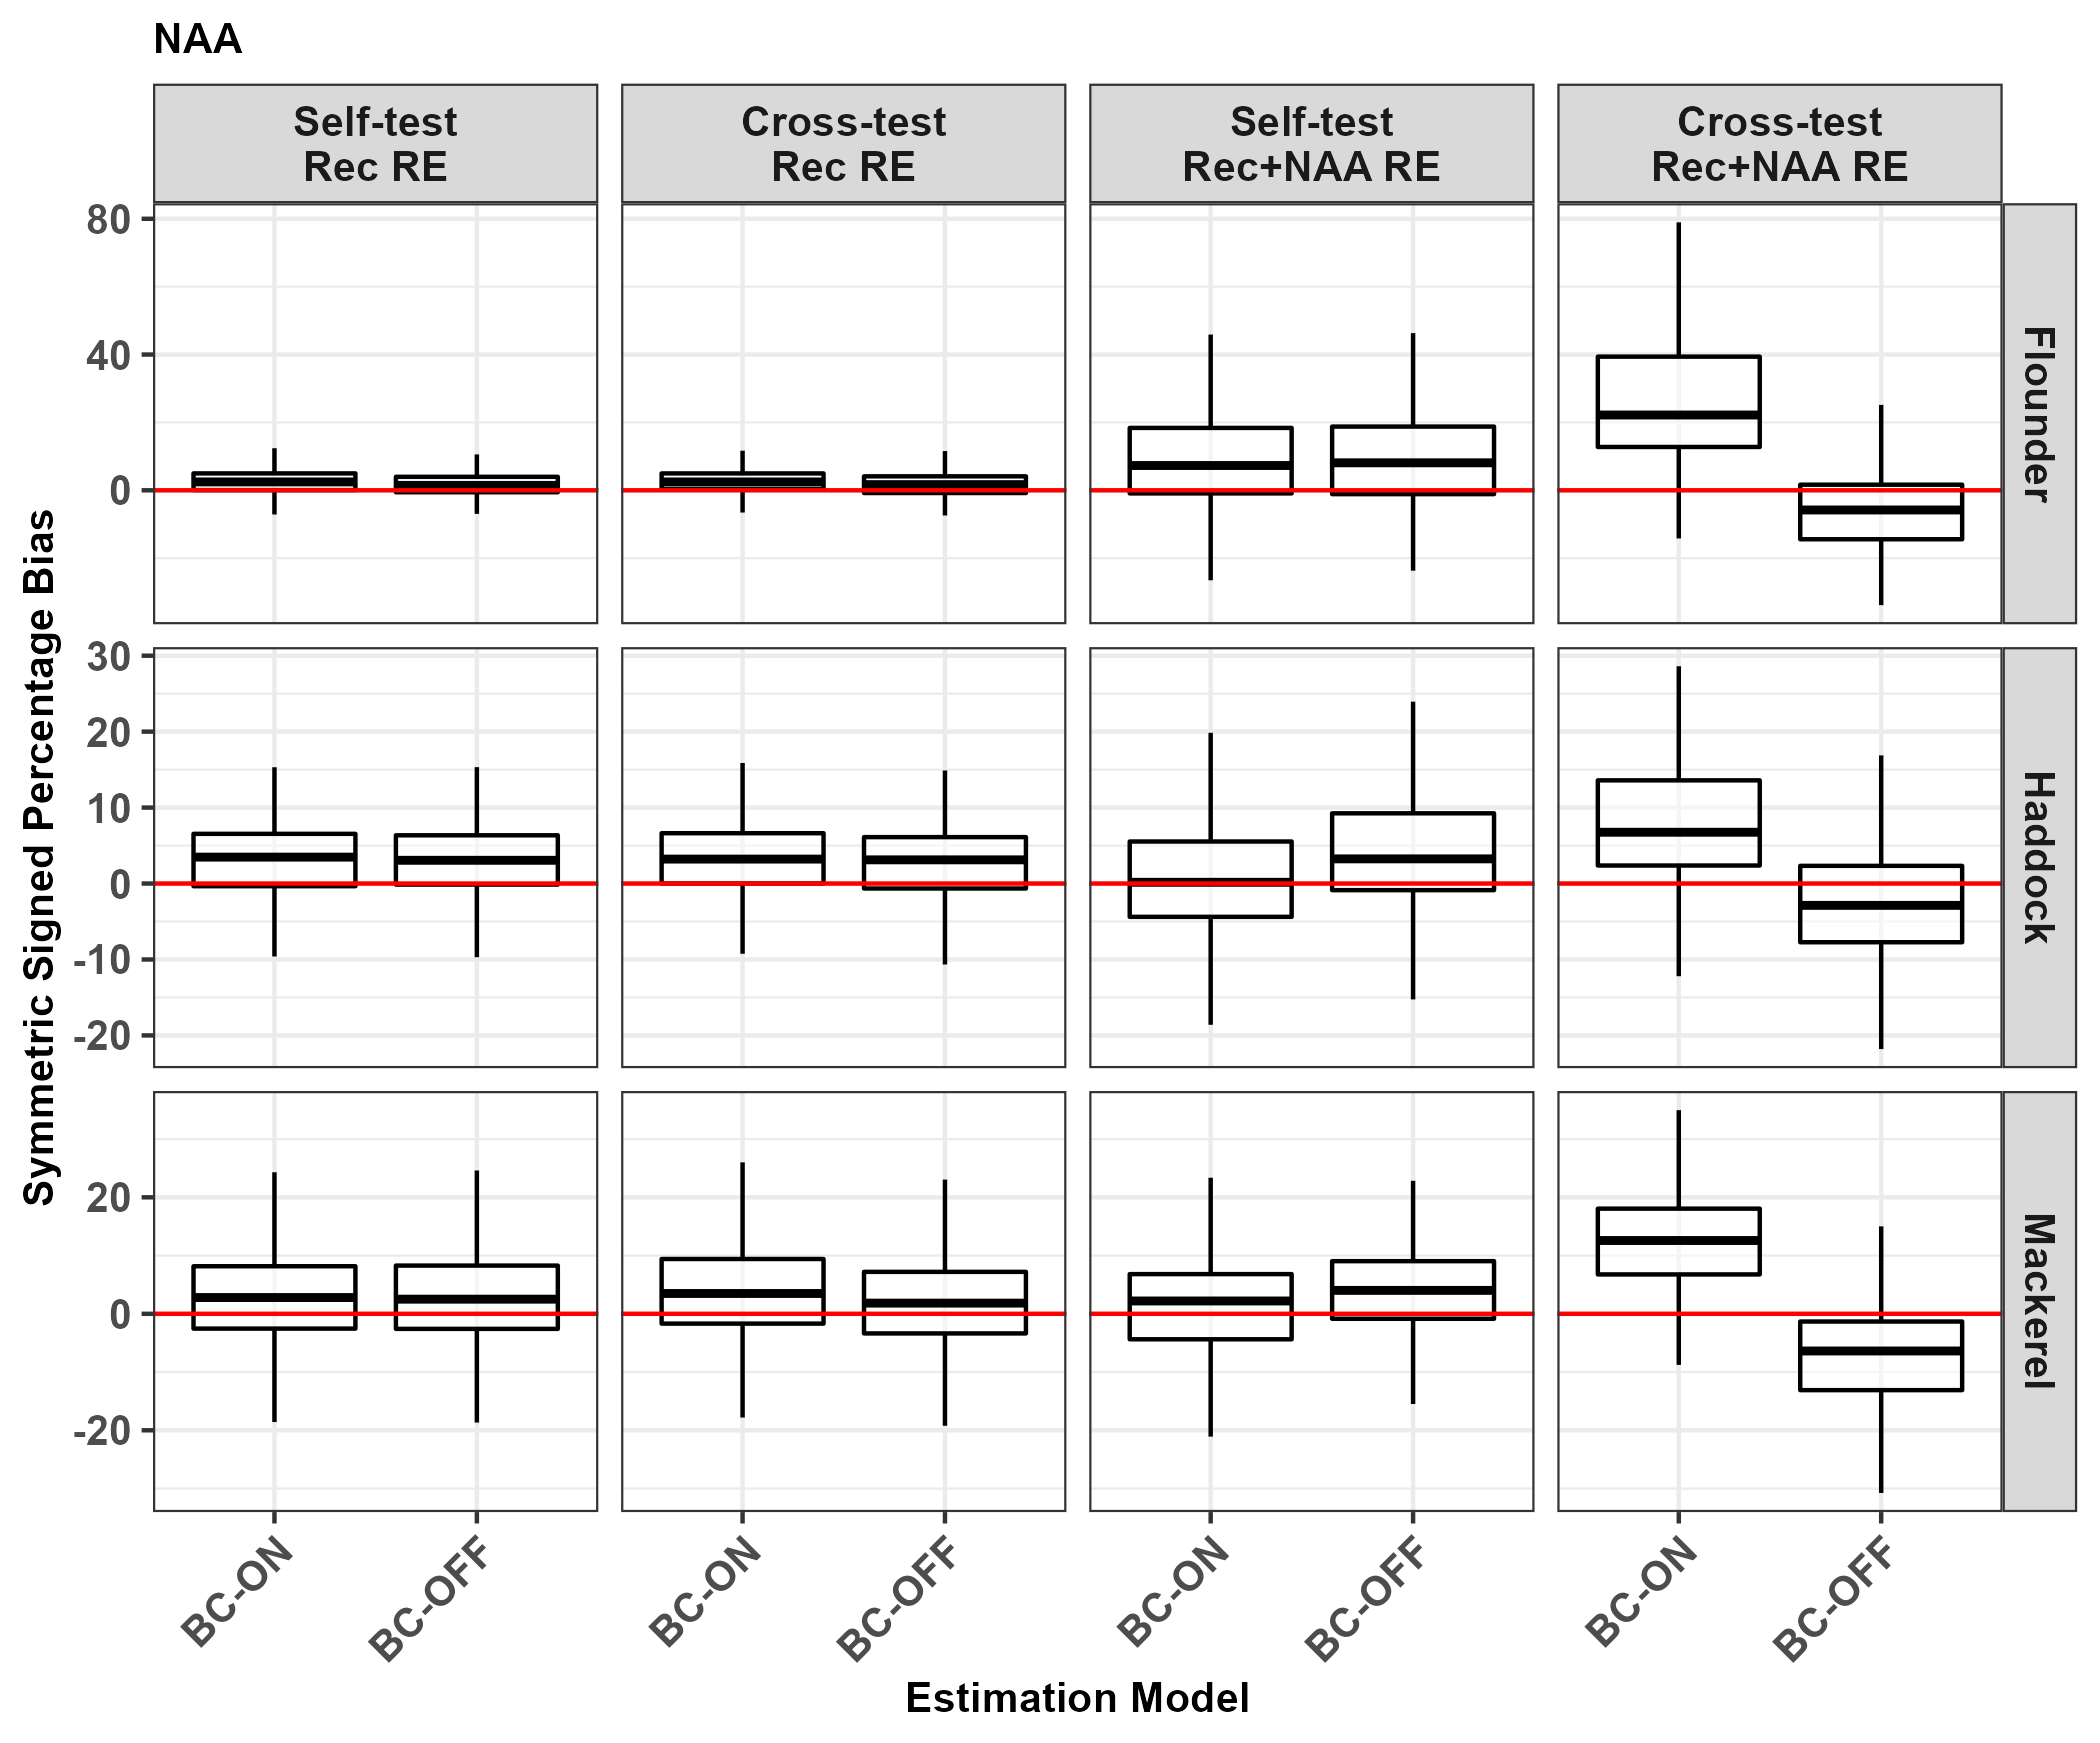
\includegraphics[width=\textwidth]{Original_Figures&Tables/Median_NAA_SSPB.PNG}
    \caption{Median symmetric signed percentage bias (SSPB) of $NAA$ calculated for self-tests and cross-tests. "Rec RE" and "Rec+NAA RE" in the top facet indicate operating models (OMs) with only recruitment random effects and both recruitment and $NAA$ random effects, respectively.}
    \label{fig:supp_NAA_SSPB}
\end{figure}

\begin{figure}[H]
    \centering
    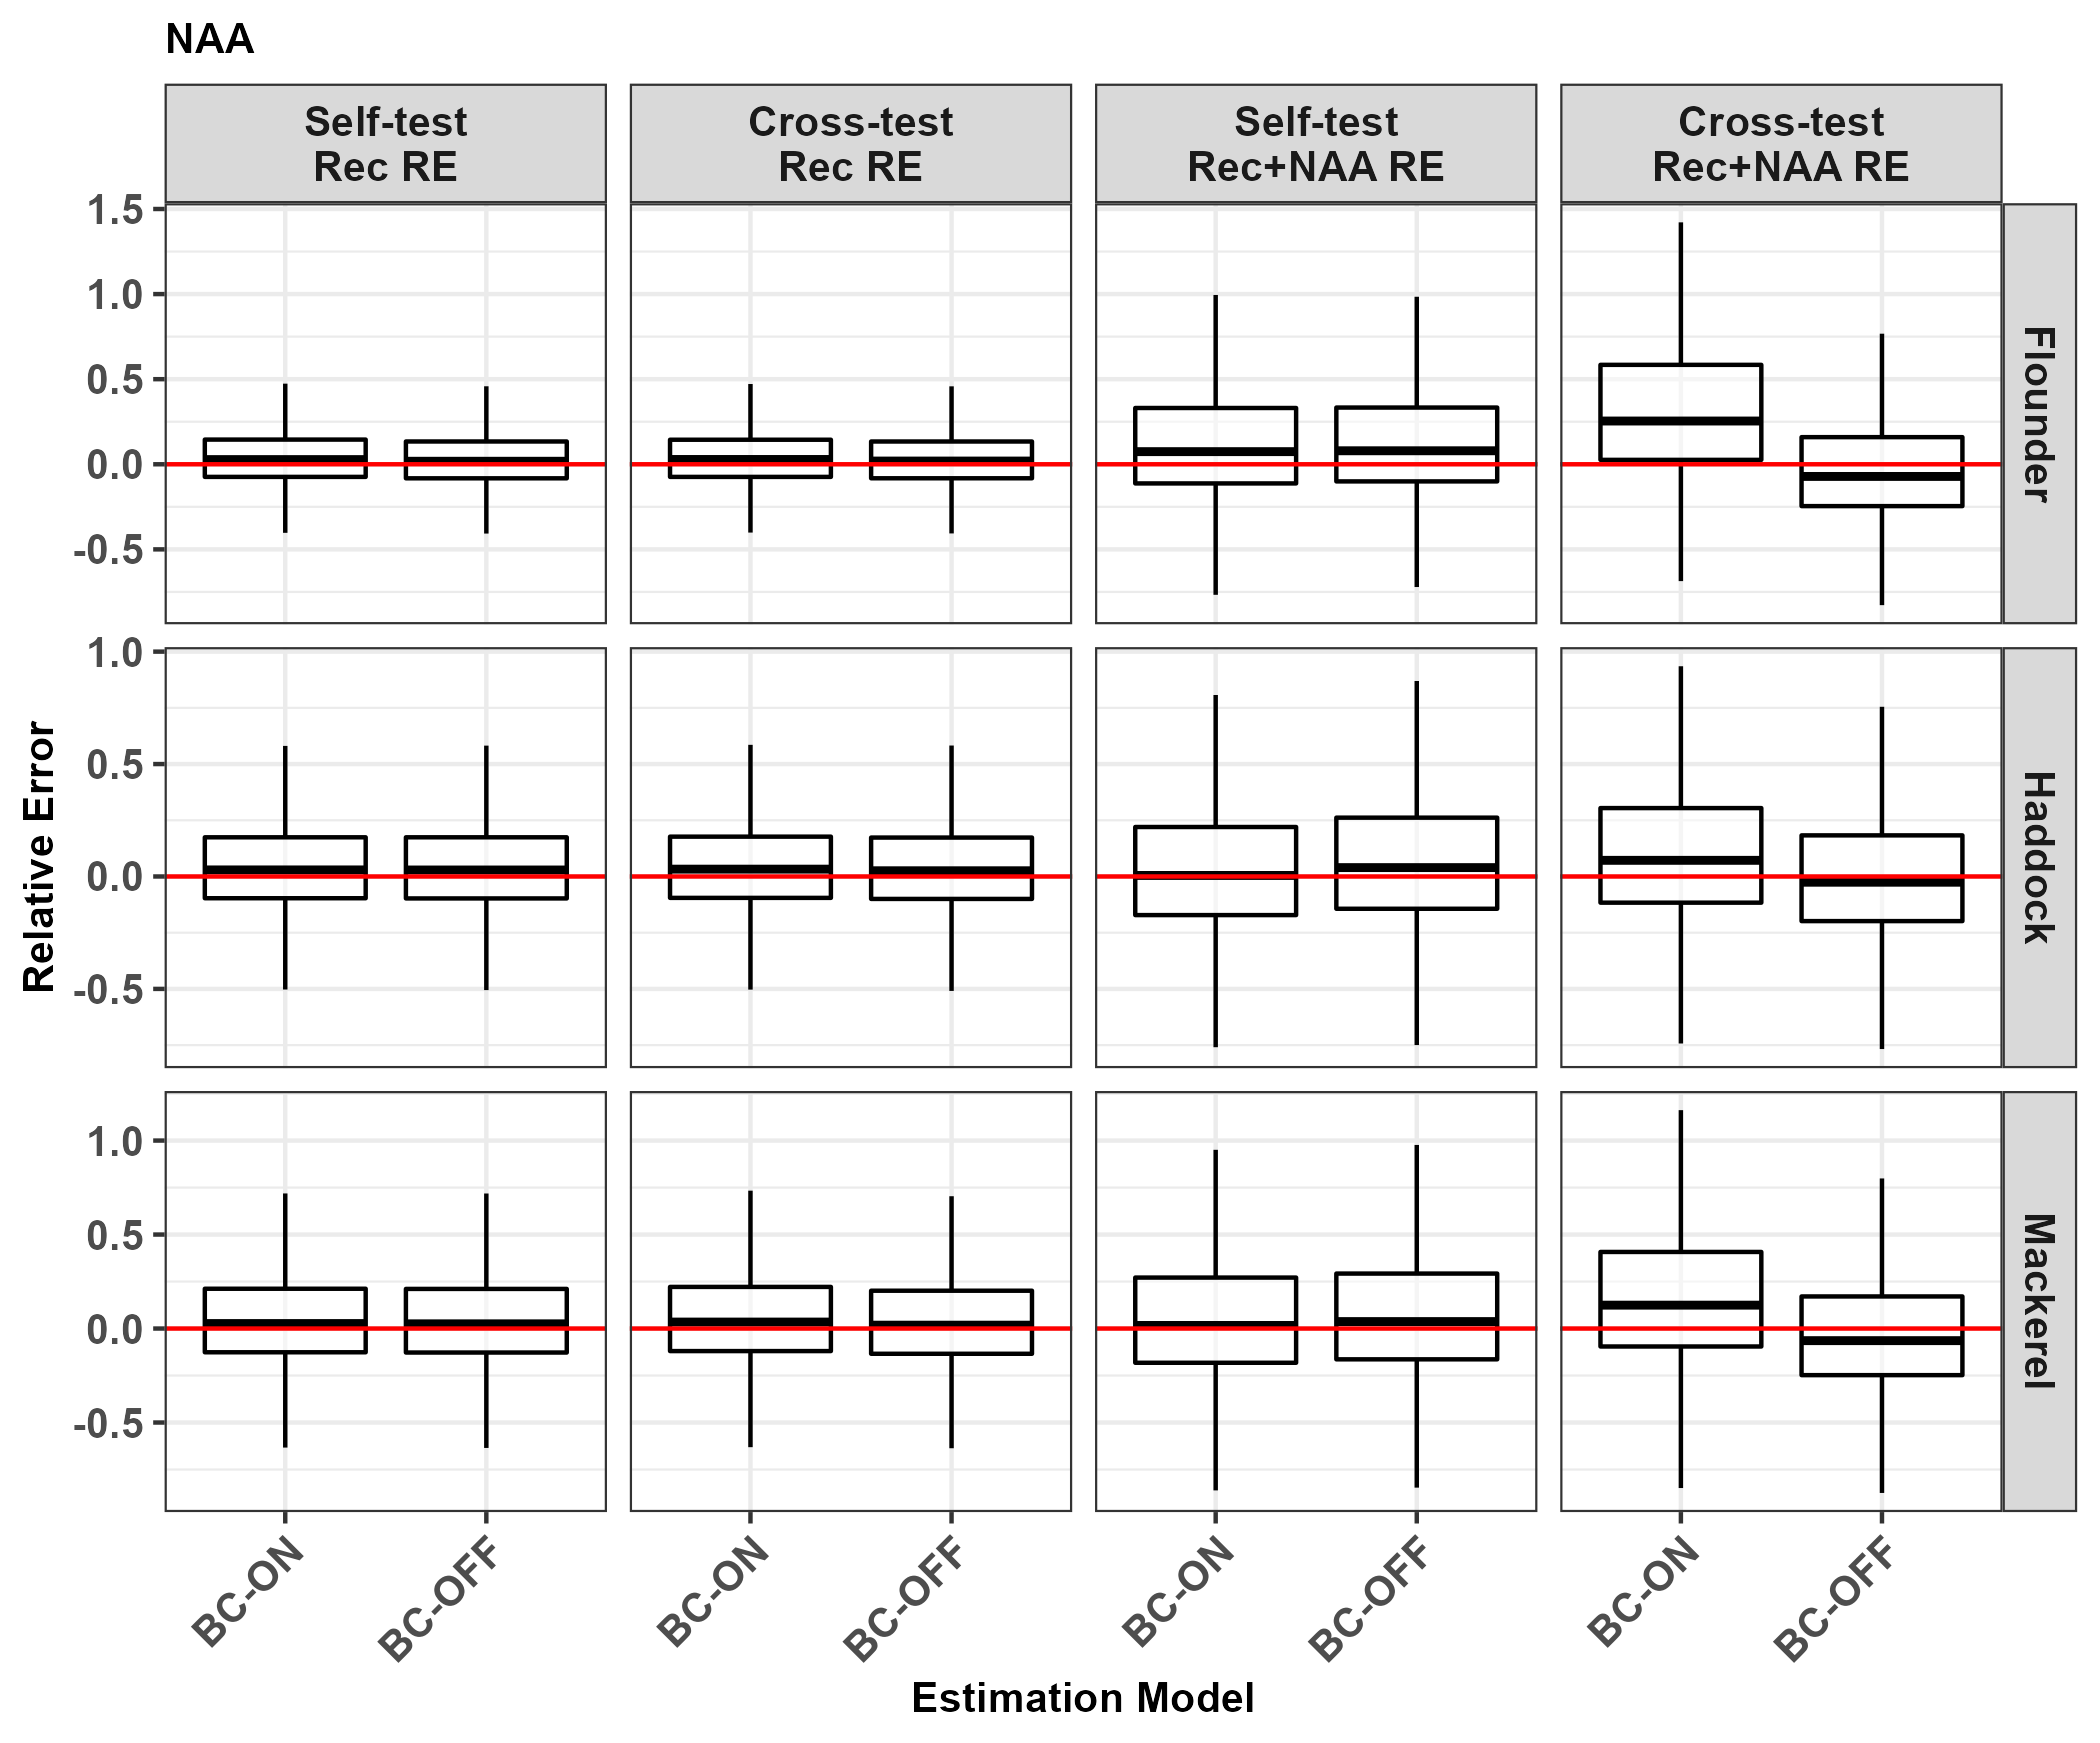
\includegraphics[width=\textwidth]{Original_Figures&Tables/Median_NAA.PNG}
    \caption{Median relative error of $NAA$ calculated for self-tests and cross-tests. "Rec RE" and "Rec+NAA RE" in the top facet indicate operating models (OMs) with only recruitment random effects and both recruitment and $NAA$ random effects, respectively.}
    \label{fig:supp_Median_NAA}
\end{figure}

\begin{figure}[H]
\centering
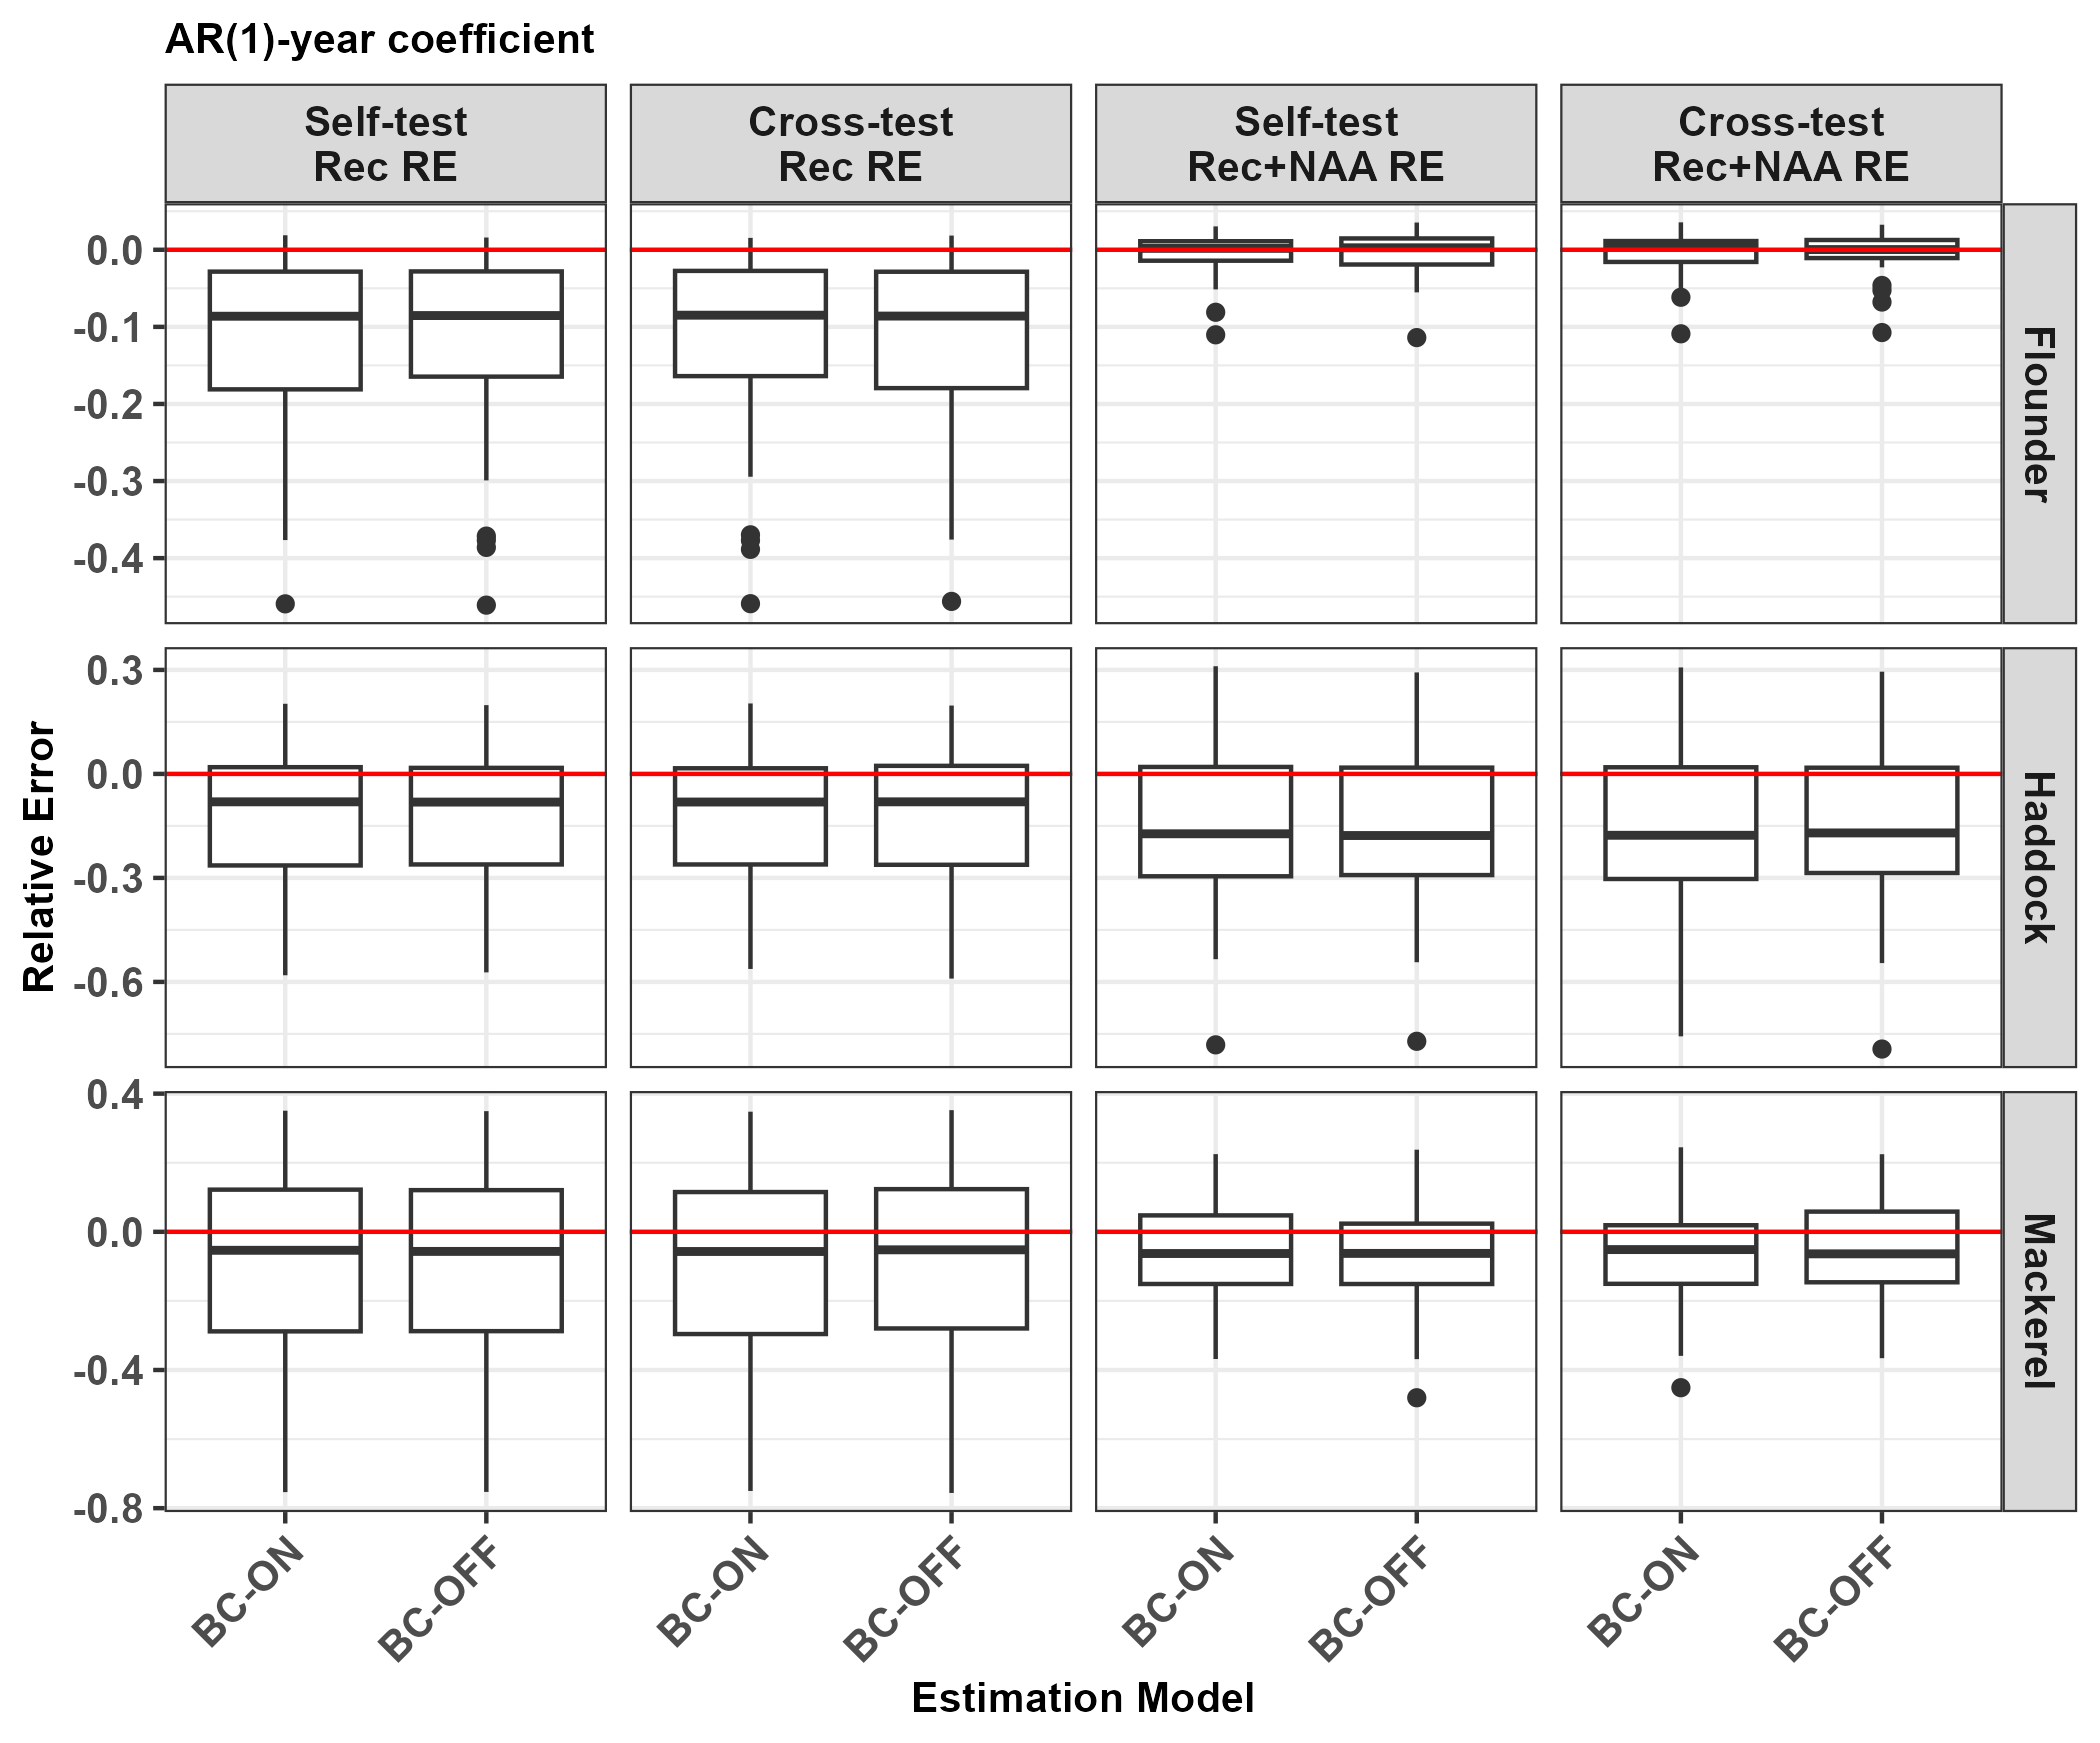
\includegraphics[width=\textwidth]{Original_Figures&Tables/Rho.PNG}
\caption{Relative error of AR(1)-year coefficient calculated for self-tests and cross-tests. "Rec RE" and "Rec+NAA RE" in the top facet indicate operating models (OMs) with only recruitment random effects and both recruitment and $NAA$ random effects, respectively.}
\label{fig:supp_ar1}
\end{figure}

\begin{figure}[H]
    \centering
    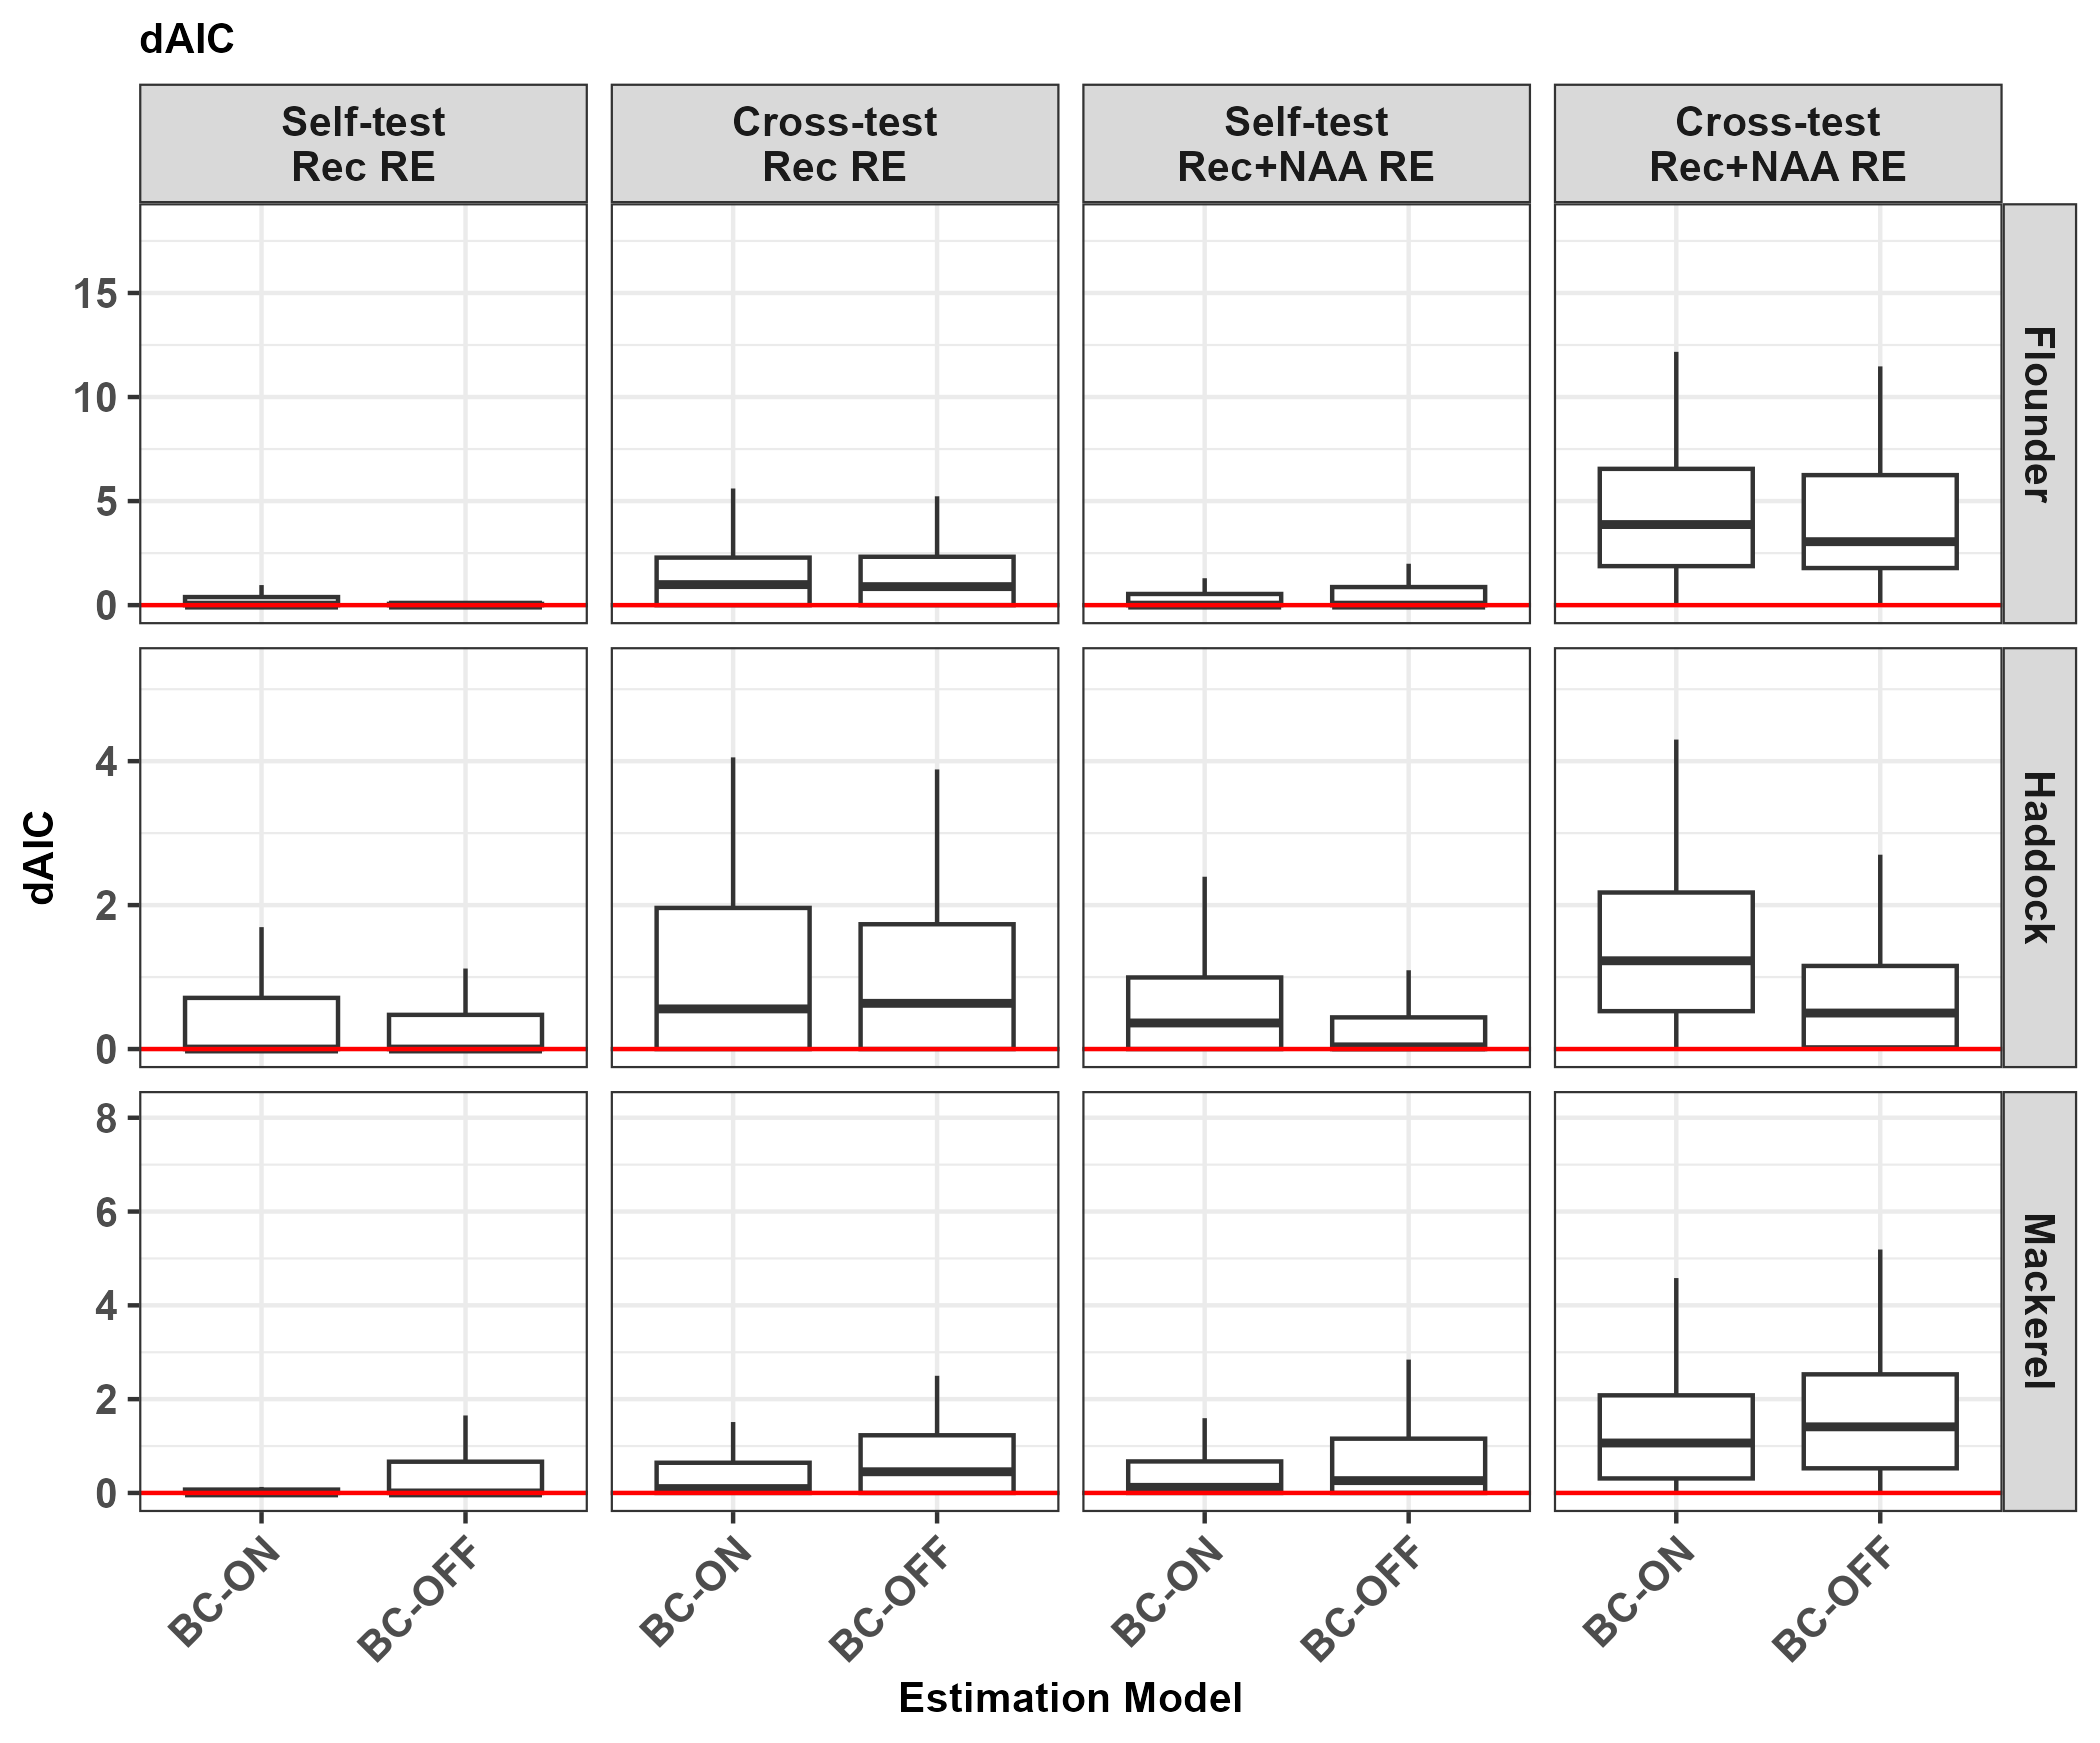
\includegraphics[width=\textwidth]{Original_Figures&Tables/dAIC.PNG}
    \caption{dAIC calculated for self-tests and cross-tests. "Rec RE" and "Rec+NAA RE" in the top facet indicate operating models (OMs) with only recruitment random effects and both recruitment and $NAA$ random effects, respectively.}
    \label{fig:supp_dAIC}
\end{figure}

\begin{figure}[H]
    \centering
    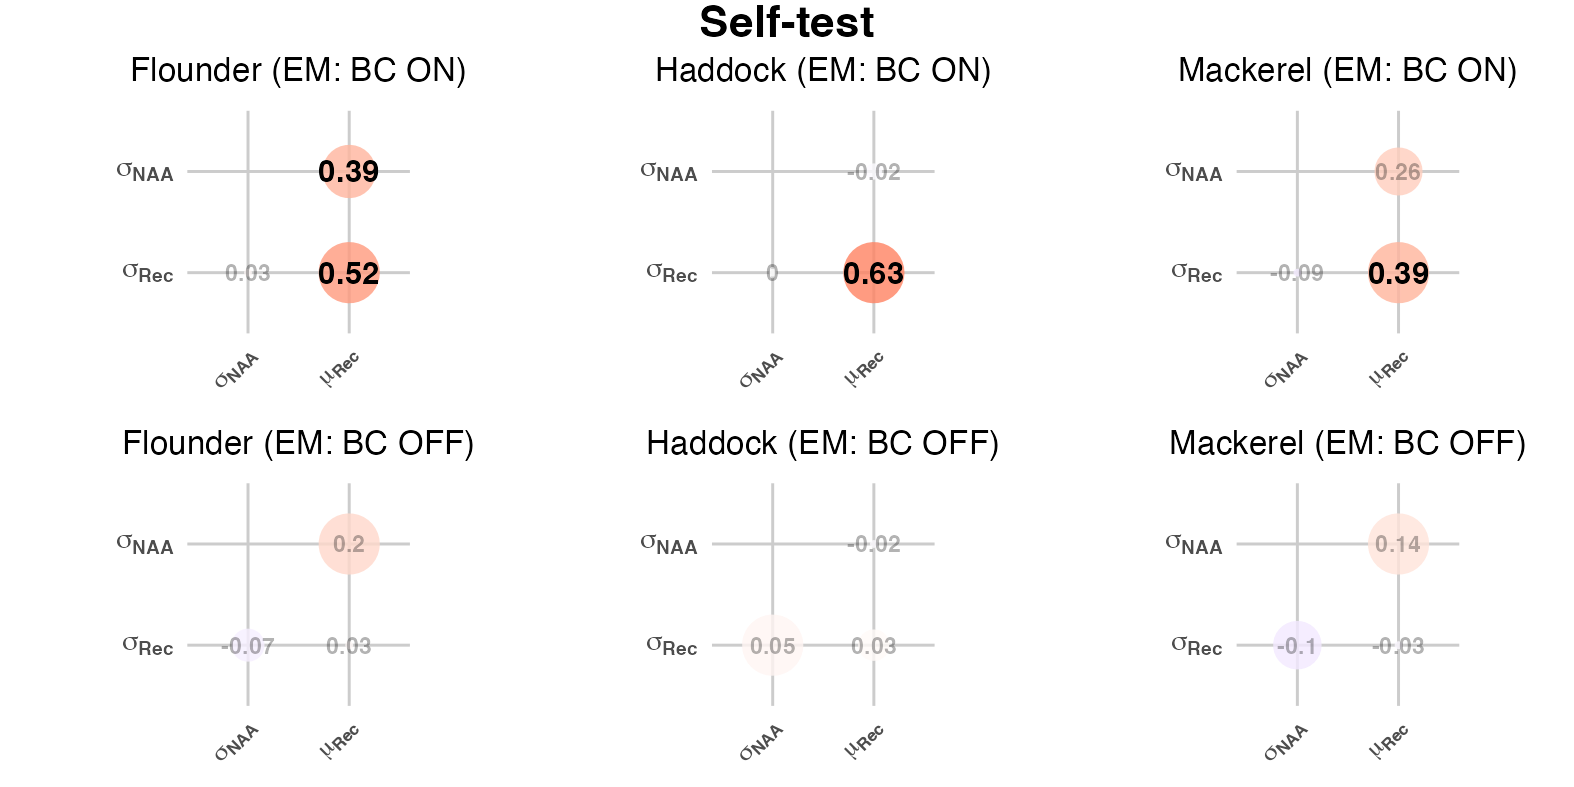
\includegraphics[width=\textwidth]{Original_Figures&Tables/Correlation_plot_NAA_iid.PNG}
    \caption{Correlation plot for the OM with both recruitment and $NAA$ treated as IID random effects. The correlations were calculated from self-tests, where the EM had the same bias correction as the operating model (OM). Correlations in \textbf{bold} indicate statistically significant values (p-value < 0.05).}
    \label{fig:supp_Cor_NAA_iid}
\end{figure}

\begin{figure}[H]
    \centering
    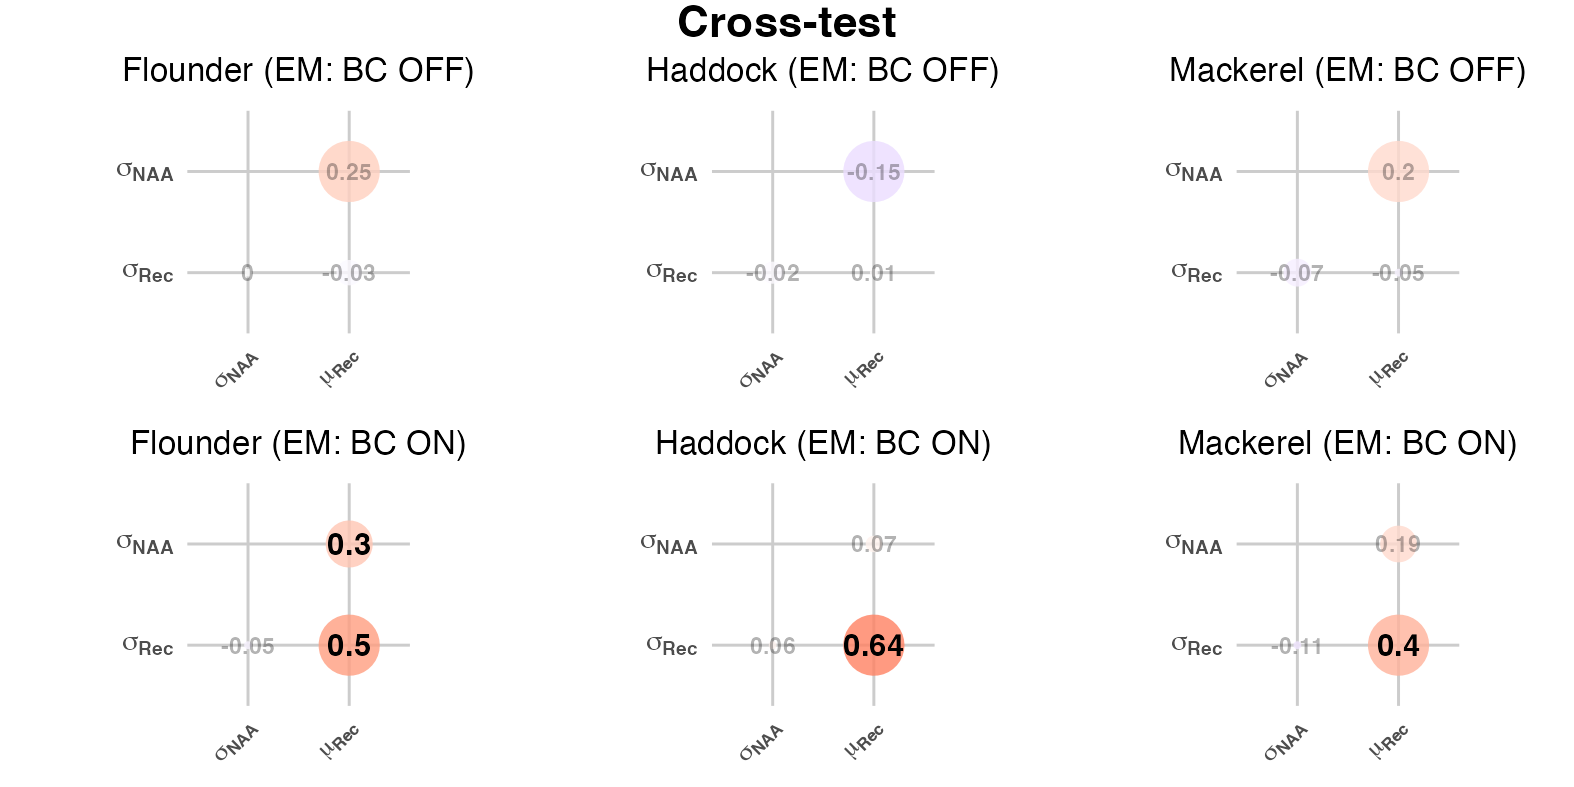
\includegraphics[width=\textwidth]{Original_Figures&Tables/Correlation_plot_NAA_iid_mismatch.PNG}
    \caption{Correlation plot for the OM with both recruitment and $NAA$ treated as IID random effects. The correlations were calculated from cross-tests, where the EM had a different bias correction than the operating model (OM). Correlations in \textbf{bold} indicate statistically significant values (p-value < 0.05).}
    \label{fig:supp_Cor_NAA_iid_mis}
\end{figure}

\begin{figure}[H]
\centering
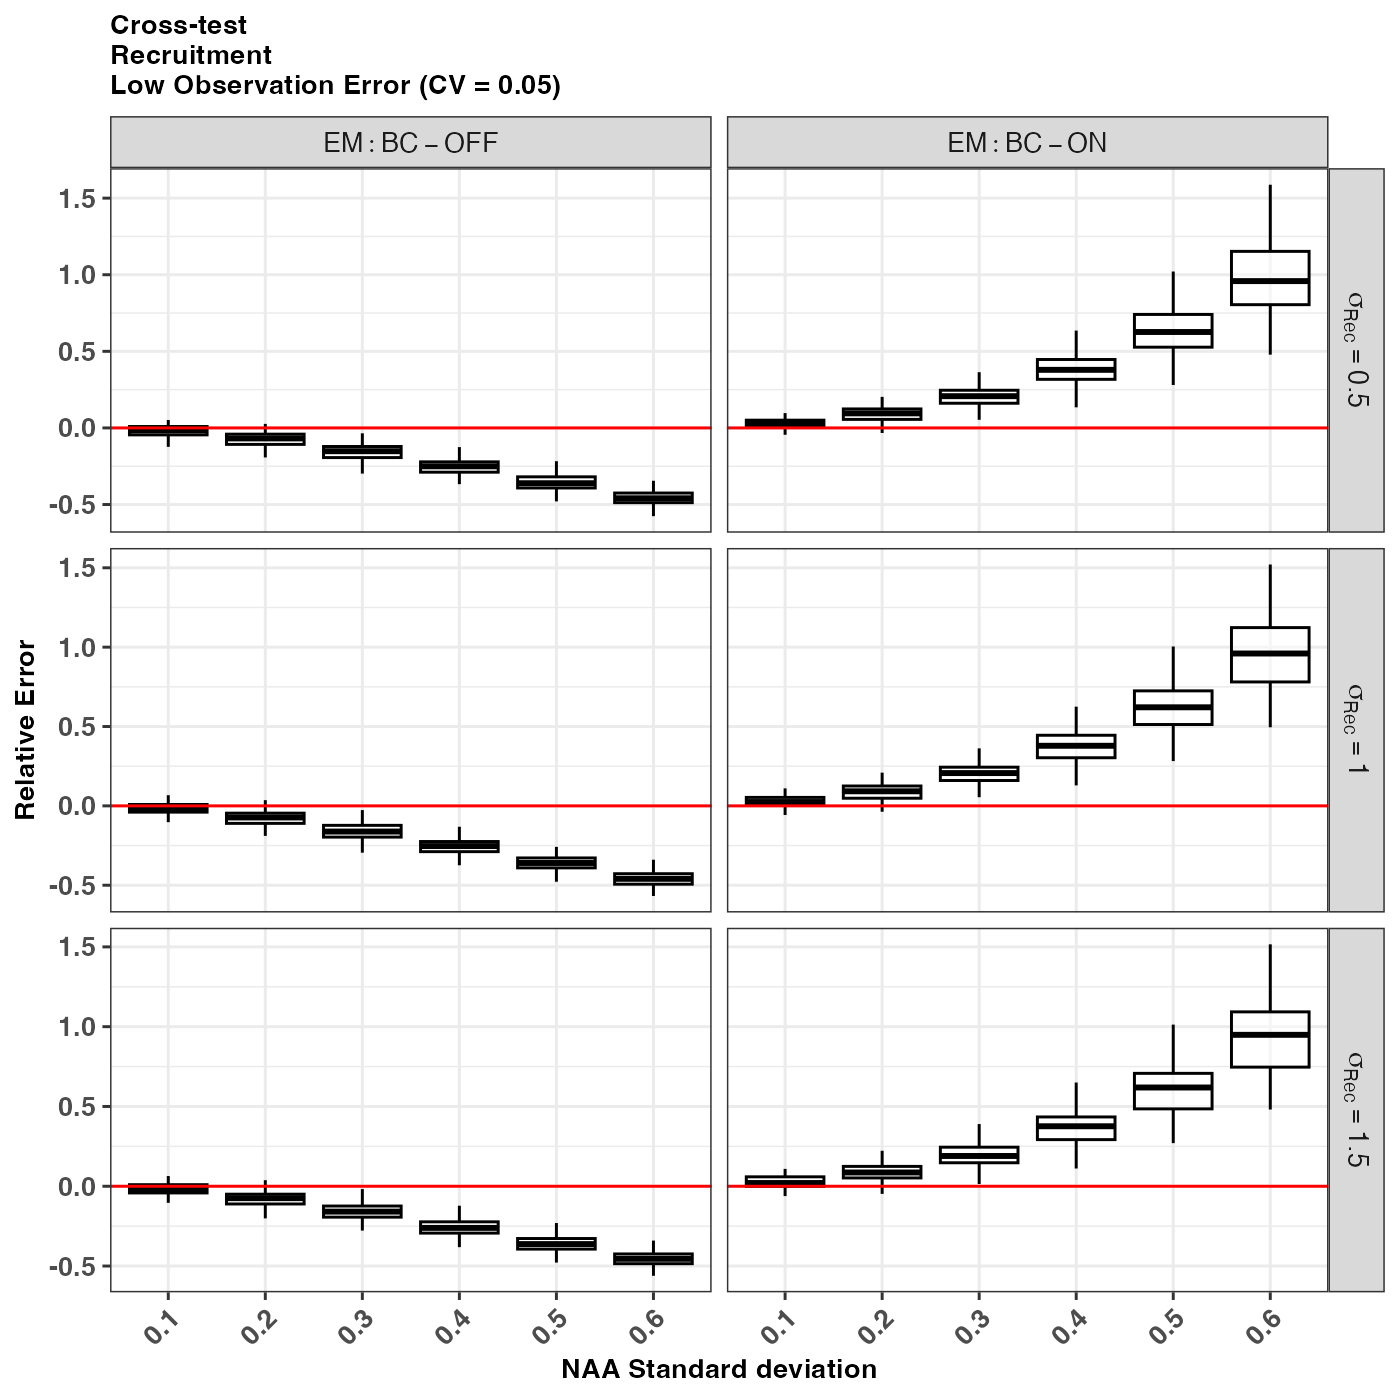
\includegraphics[width=\textwidth]{Original_Figures&Tables/Recruitment_low_cross_RE.PNG}
\caption{Relative errors of recruitment estimates summarized from 50 realizations for each scenario. Two operating models (OMs) (with bias correction applied or omitted for both processes and observations) for Gulf of Maine (GoM) haddock with both recruitment and $NAA$ IID random effects (see Table S2) were used to conduct simulation-estimation experiments. The study evaluated the effects of recruitment variability ($\sigma_{Rec}$ = 0.5, 1, 1.5) and $NAA$ variability ($\sigma_{NAA}$ = 0.1, 0.2, ... 0.6) in a factorial design through self-tests and cross-tests. To isolate the impact of observation error, the coefficient of variation (CV) for observations was set to 0.05.}
\label{fig:supp_Recruitment_low_cross_RE}
\end{figure}

\begin{figure}[H]
\centering
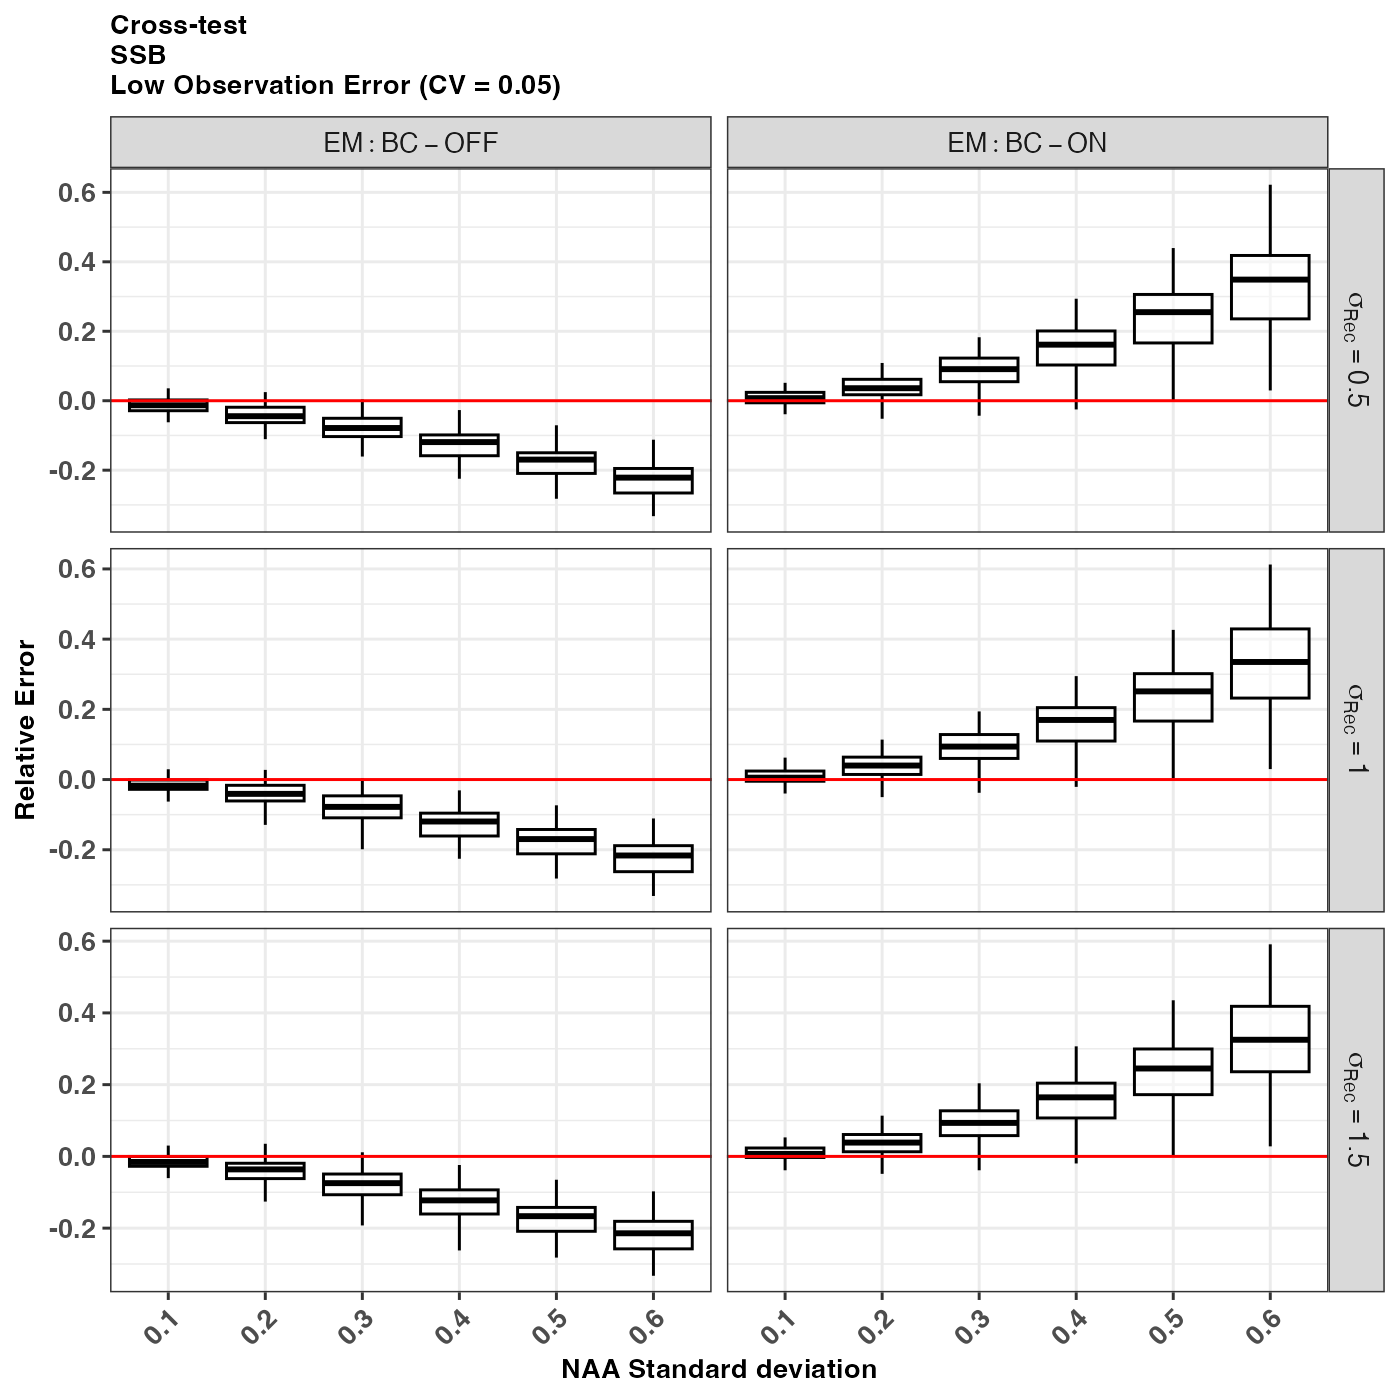
\includegraphics[width=\textwidth]{Original_Figures&Tables/SSB_low_cross_RE.PNG}
\caption{Relative errors of recruitment estimates summarized from 50 realizations for each scenario. Two operating models (OMs) (with bias correction applied or omitted for both processes and observations) for Gulf of Maine (GoM) haddock with both recruitment and $NAA$ IID random effects (see Table S2) were used to conduct simulation-estimation experiments. The study evaluated the effects of recruitment variability ($\sigma_{Rec}$ = 0.5, 1, 1.5) and $NAA$ variability ($\sigma_{NAA}$ = 0.1, 0.2, ... 0.6) in a factorial design through self-tests and cross-tests. To isolate the impact of observation error, the coefficient of variation (CV) for observations was set to 0.05.}
\label{fig:supp_SSB_low_cross_RE} 
\end{figure}

\begin{figure}[H]
\centering
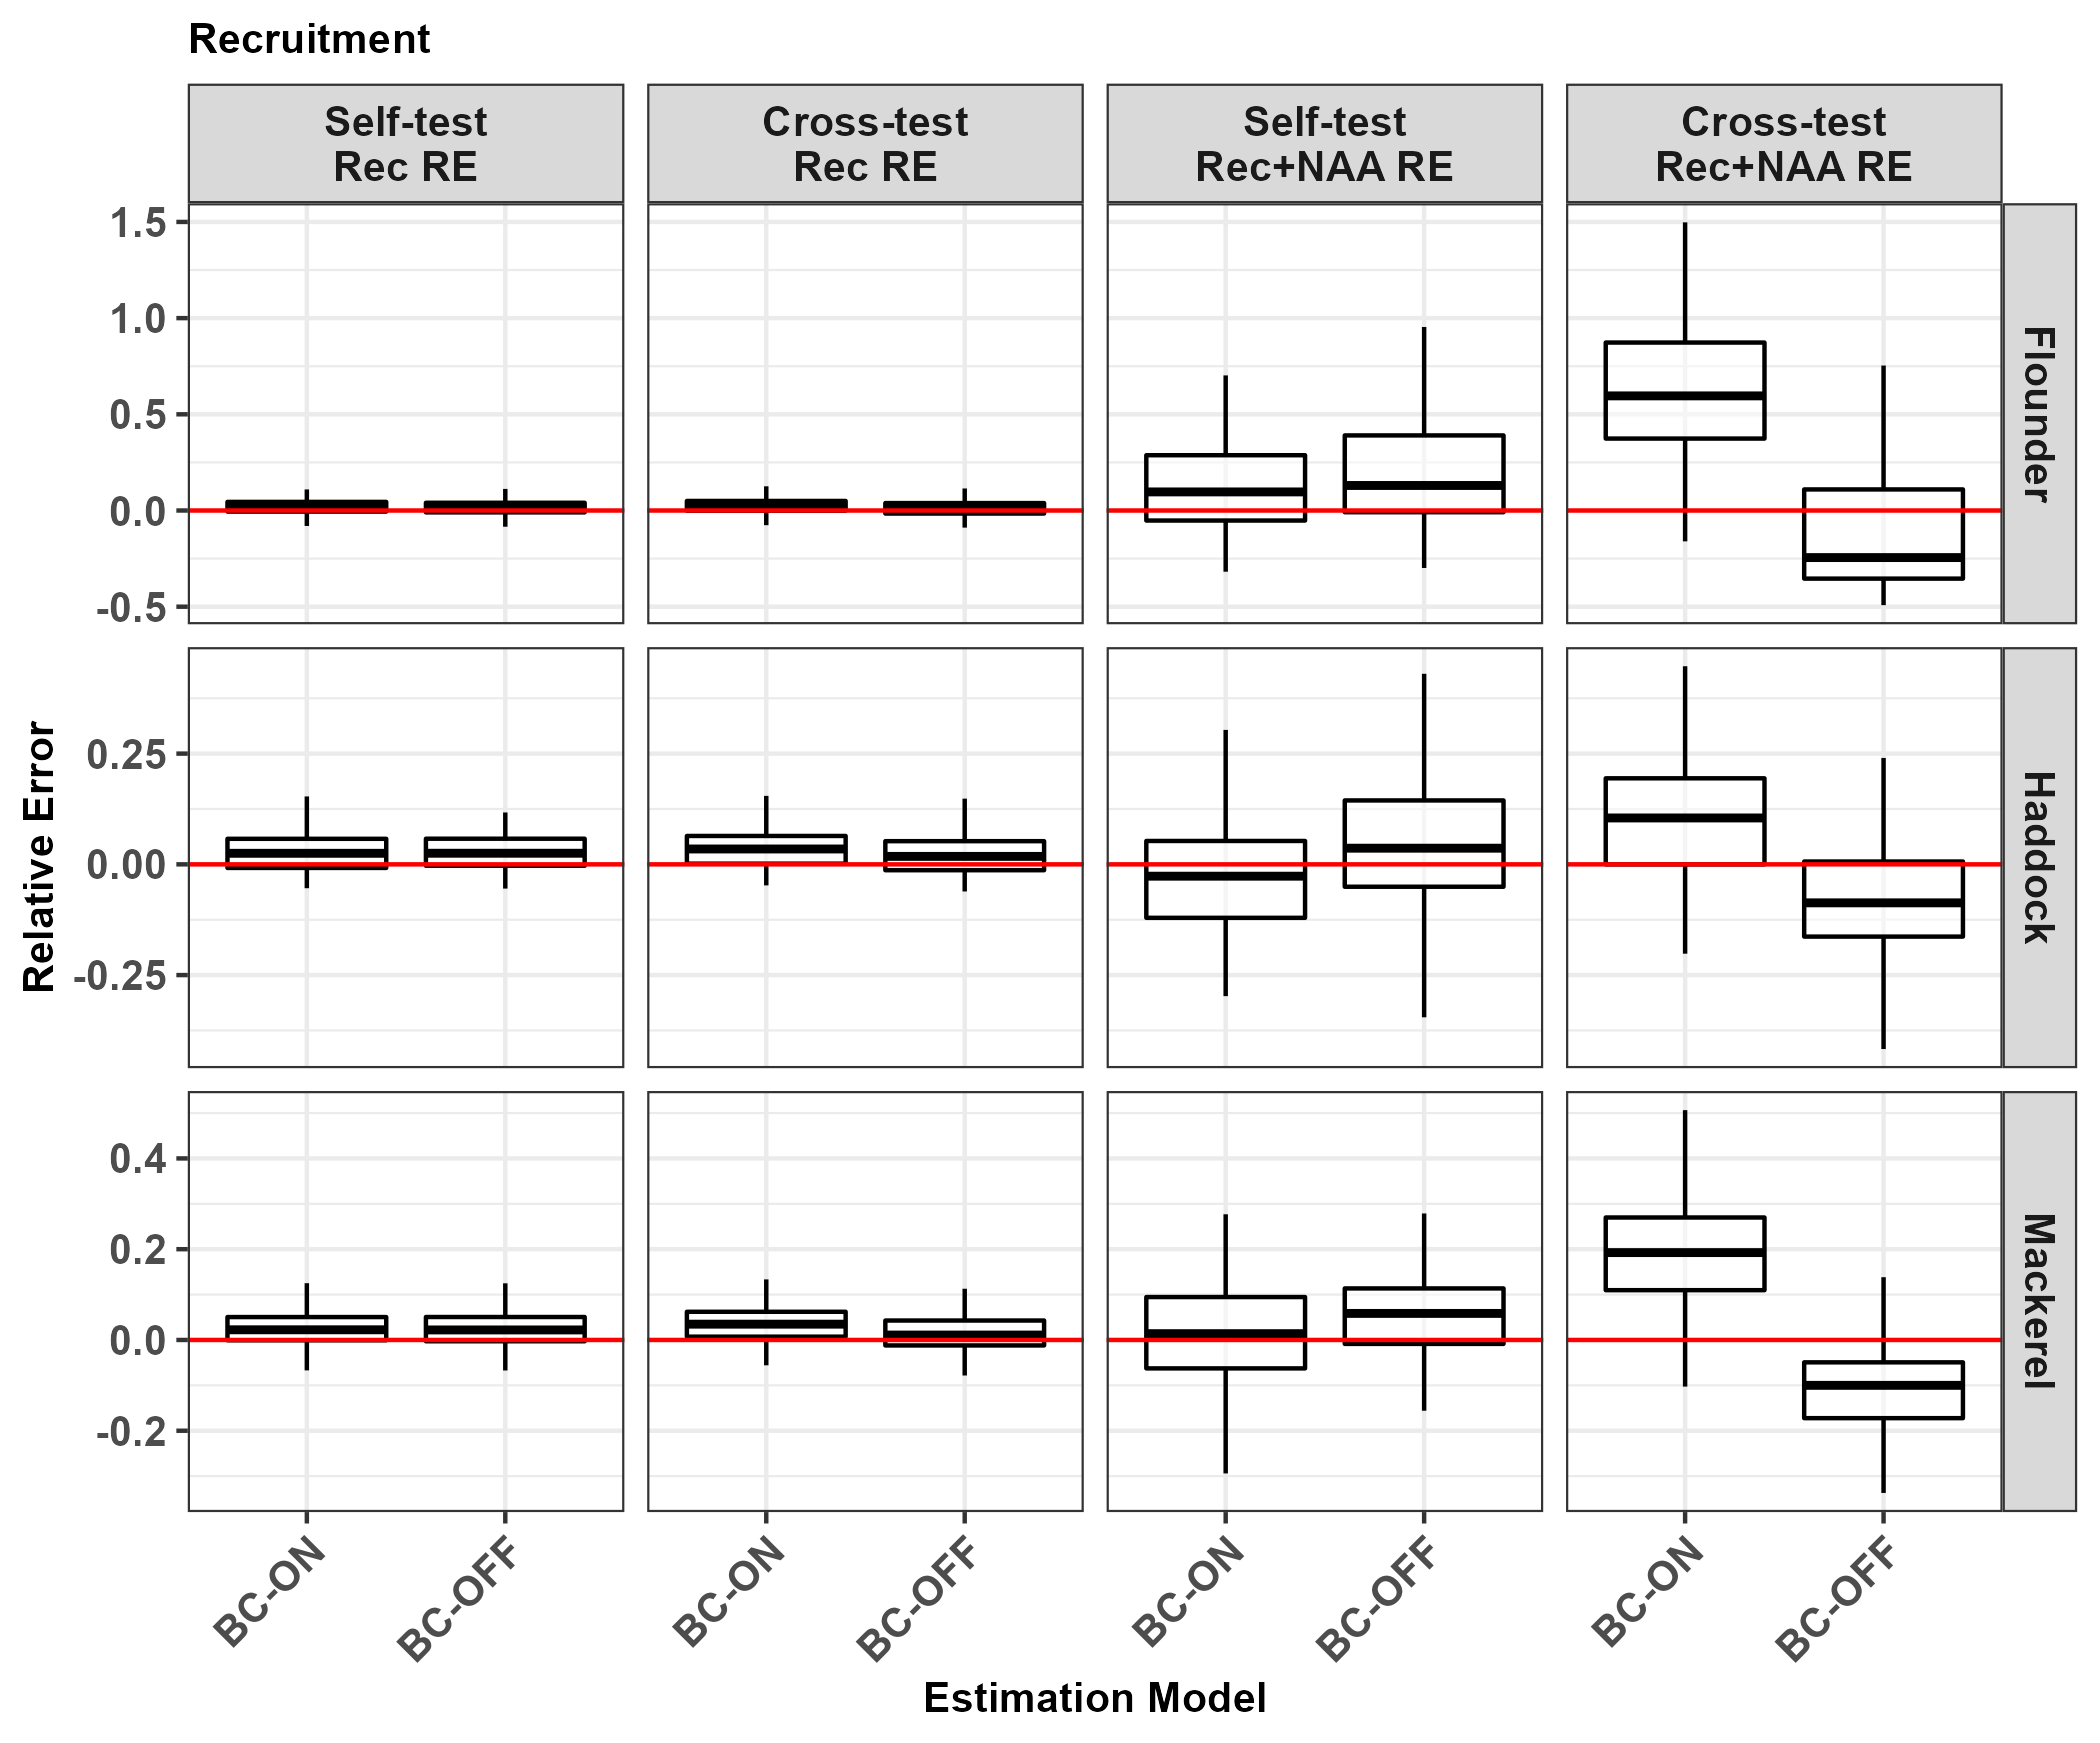
\includegraphics[width=\textwidth]{Original_Figures&Tables/Rec_intermediate.PNG}
\caption{Median relative eror of recruitment in the intermediate period (with first and last 10 years of estiamtes removed).}
\label{fig:supp_Rec_intermediate}
\end{figure}

\begin{figure}[H]
\centering
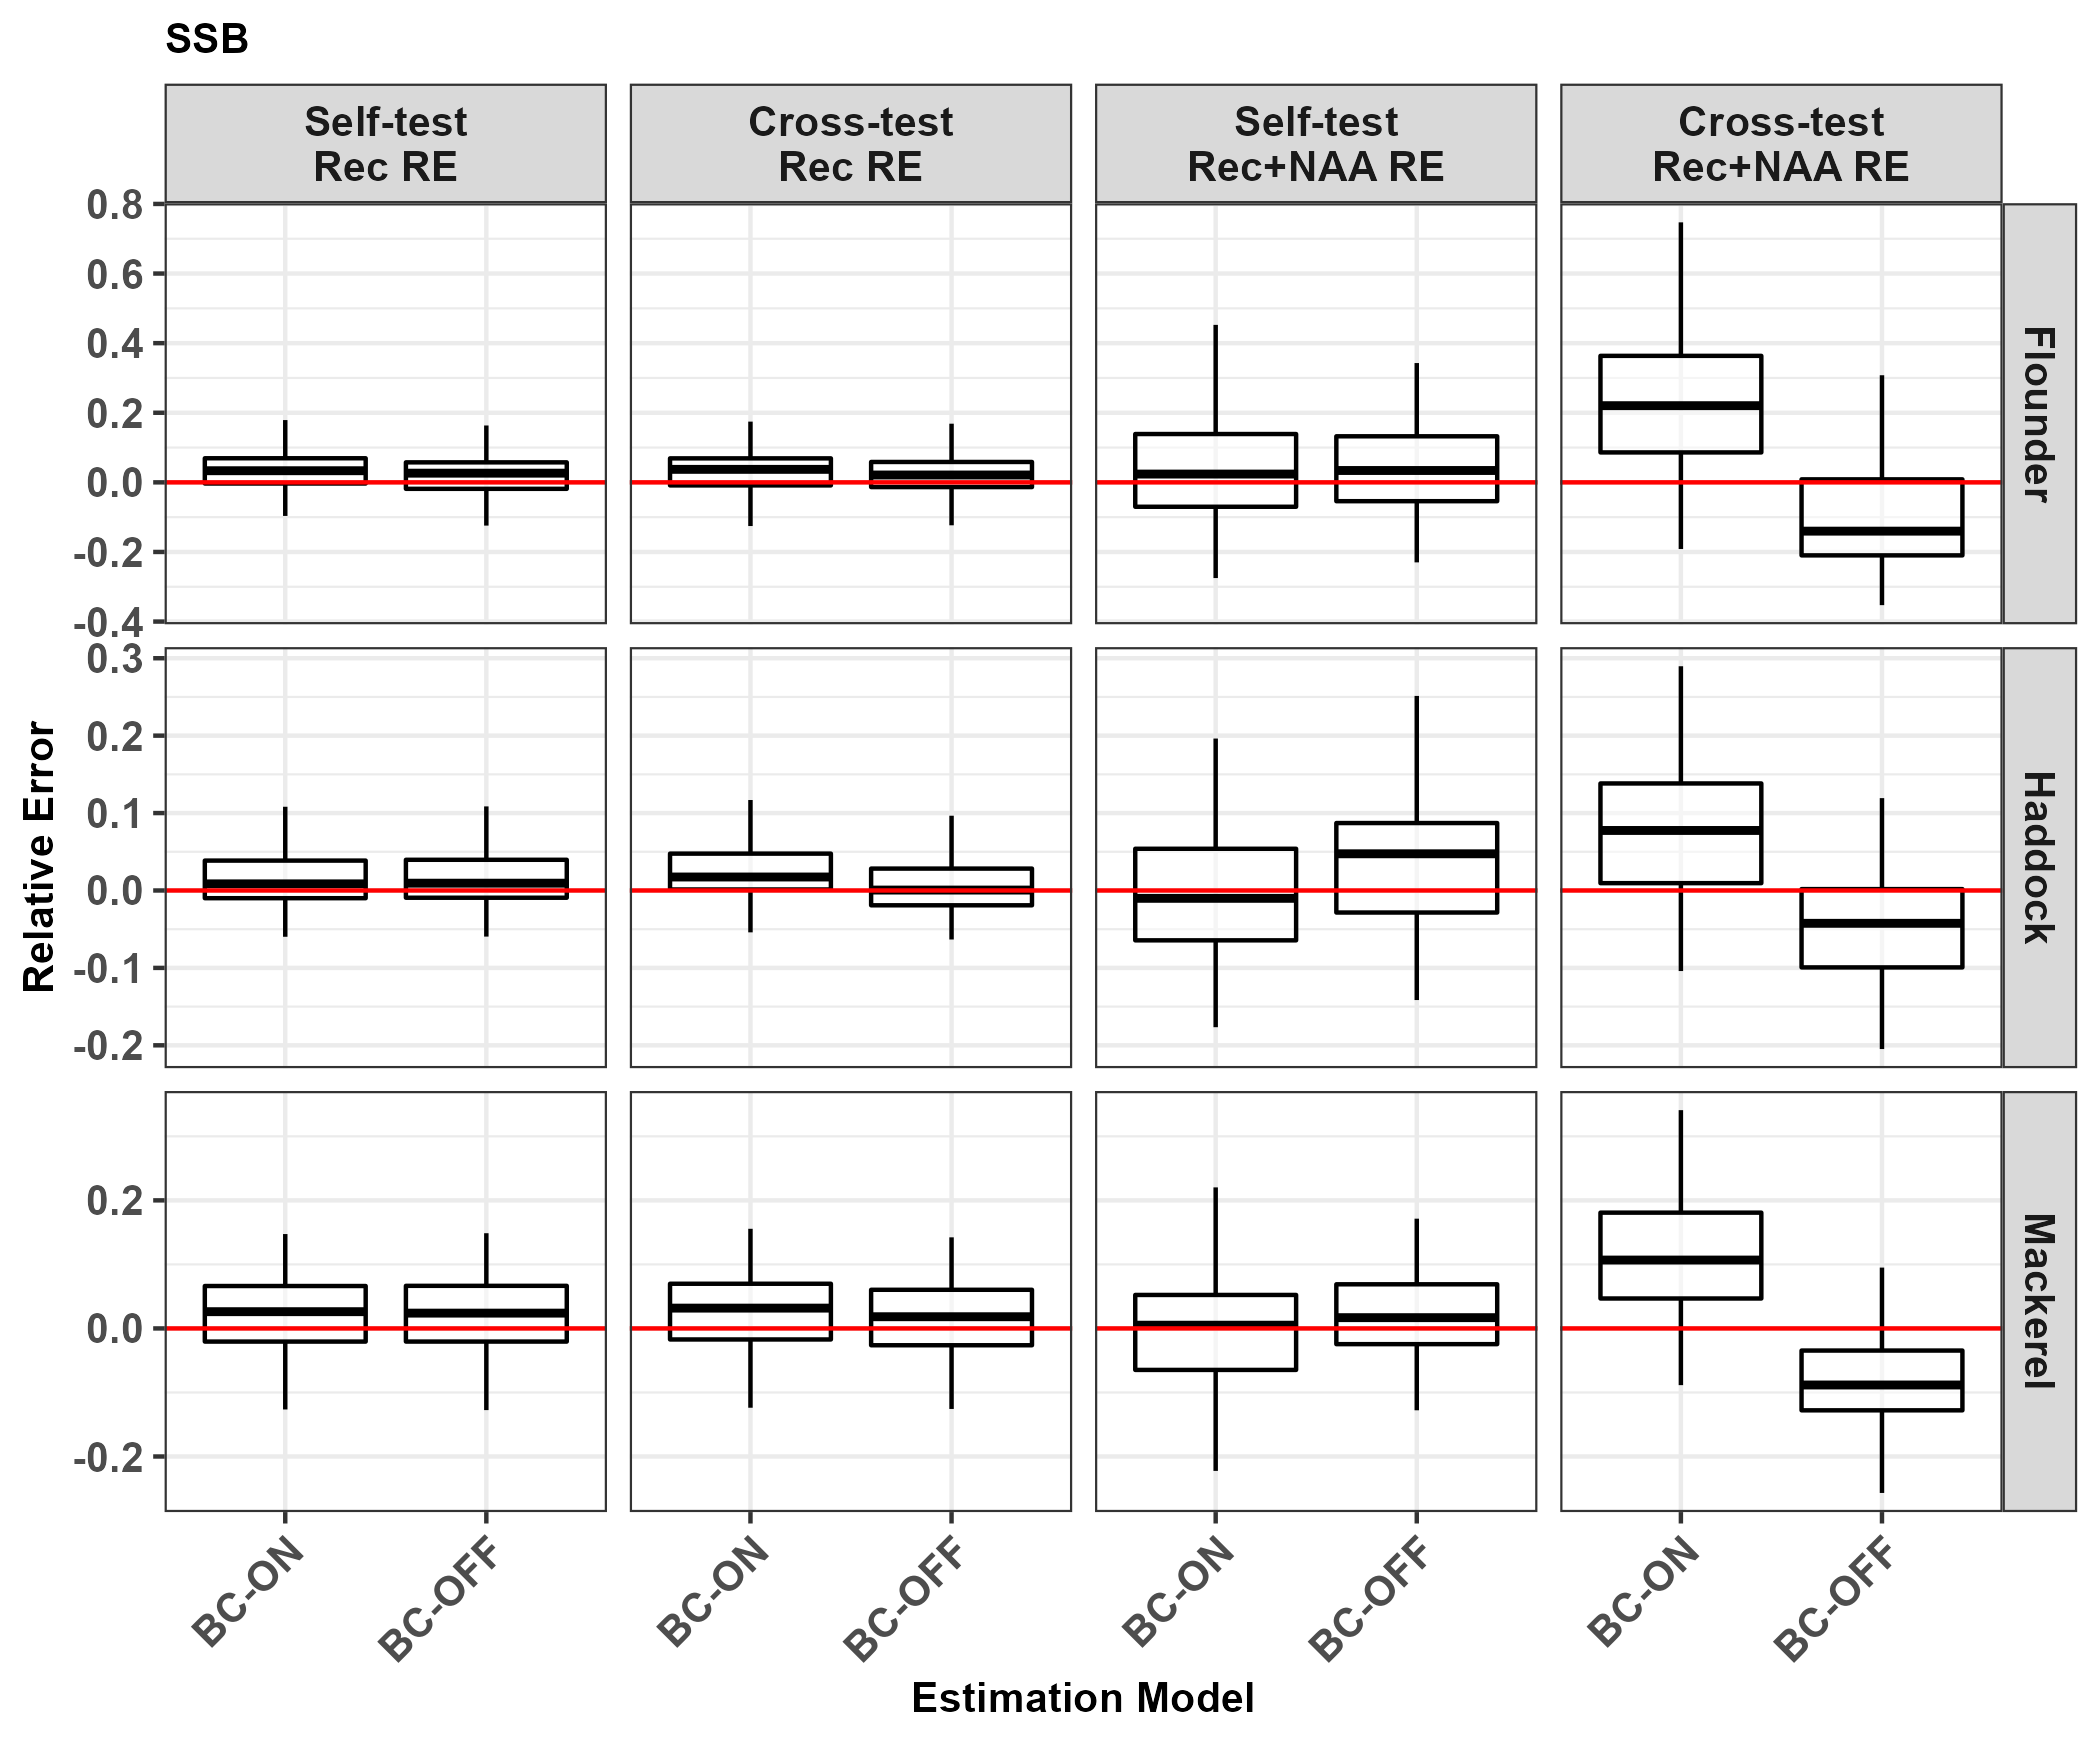
\includegraphics[width=\textwidth]{Original_Figures&Tables/SSB_intermediate.PNG}
\caption{Median relative eror of $SSB$ in the intermediate period (with first and last 10 years of estiamtes removed).}
\label{fig:supp_SSB_intermediate}
\end{figure}

\renewcommand{\thefigure}{\arabic{figure}}

\pagebreak

\bibliography{paper}

\pagebreak

\end{document}
